%\DeclareUnicodeCharacter{2212}{-}
%&preformat-disser
%\RequirePackage[l2tabu,orthodox]{nag} % Раскомментировав, можно в логе получать рекомендации относительно правильного использования пакетов и предупреждения об устаревших и нерекомендуемых пакетах
% Формат А4, 14pt (ГОСТ Р 7.0.11-2011, 5.3.6)
\documentclass[a4paper,14pt,oneside,openany]{memoir}

%%%%%%%%%%%%%%%%%%%%%%%%%%%%%%%%%%%%%%%%%%%%%%%%%%%%%%%%%%%%%%%%%%%%%%%%%%%%%%%%
%%%% Файл упрощённых настроек шаблона, общих для диссертации и автореферата %%%%
%%%%%%%%%%%%%%%%%%%%%%%%%%%%%%%%%%%%%%%%%%%%%%%%%%%%%%%%%%%%%%%%%%%%%%%%%%%%%%%%

%%% Режим черновика %%%
\makeatletter
\@ifundefined{c@draft}{
  \newcounter{draft}
  \setcounter{draft}{0}  % 0 --- чистовик (максимальное соблюдение ГОСТ)
                         % 1 --- черновик (отклонения от ГОСТ, но быстрая
                         %       сборка итоговых PDF)
}{}
\makeatother

%%% Пометки в тексте %%%
\makeatletter
\@ifundefined{c@showmarkup}{
  \newcounter{showmarkup}
  \setcounter{showmarkup}{0}  % 0 --- скрыть пометки
                              % 1 --- показывать пометки
}{}
\makeatother

%%% Использование в pdflatex шрифтов не по-умолчанию %%%
\makeatletter
\@ifundefined{c@usealtfont}{
  \newcounter{usealtfont}
  \setcounter{usealtfont}{1}    % 0 --- шрифты на базе Computer Modern
                                % 1 --- использовать пакет pscyr, при его
                                %       наличии
                                % 2 --- использовать пакет XCharter, при наличии
                                %       подходящей версии
}{}
\makeatother

%%% Использование в xelatex и lualatex семейств шрифтов %%%
\makeatletter
\@ifundefined{c@fontfamily}{
  \newcounter{fontfamily}
  \setcounter{fontfamily}{1}  % 0 --- CMU семейство. Используется как fallback;
                              % 1 --- Шрифты от MS (Times New Roman и компания)
                              % 2 --- Семейство Liberation
}{}
\makeatother

%%% Библиография %%%
\makeatletter
\@ifundefined{c@bibliosel}{
  \newcounter{bibliosel}
  \setcounter{bibliosel}{1}   % 0 --- встроенная реализация с загрузкой файла
                              %       через движок bibtex8;
                              % 1 --- реализация пакетом biblatex через движок
                              %       biber
}{}
\makeatother

%%% Вывод типов ссылок в библиографии %%%
\makeatletter
\@ifundefined{c@mediadisplay}{
  \newcounter{mediadisplay}
  \setcounter{mediadisplay}{1}   % 0 --- не делать ничего; надписи [Текст] и
                                 %       [Эл. ресурс] будут выводиться только в ссылках с
                                 %       заполненным полем `media`;
                                 % 1 --- автоматически добавлять надпись [Текст] к ссылкам с
                                 %       незаполненным полем `media`; таким образом, у всех
                                 %       источников будет указан тип, что соответствует
                                 %       требованиям ГОСТ
                                 % 2 --- автоматически удалять надписи [Текст], [Эл. Ресурс] и др.;
                                 %       не соответствует ГОСТ
                                 % 3 --- автоматически удалять надпись [Текст];
                                 %       не соответствует ГОСТ
                                 % 4 --- автоматически удалять надпись [Эл. Ресурс];
                                 %       не соответствует ГОСТ
}{}
\makeatother

%%% Предкомпиляция tikz рисунков для ускорения работы %%%
\makeatletter
\@ifundefined{c@imgprecompile}{
  \newcounter{imgprecompile}
  \setcounter{imgprecompile}{0}   % 0 --- без предкомпиляции;
                                  % 1 --- пользоваться предварительно
                                  %       скомпилированными pdf вместо генерации
                                  %       заново из tikz
}{}
\makeatother
            % общие настройки шаблона
%%% Проверка используемого TeX-движка %%%
\newif\ifxetexorluatex   % определяем новый условный оператор (http://tex.stackexchange.com/a/47579)
\ifxetex
    \xetexorluatextrue
\else
    \ifluatex
        \xetexorluatextrue
    \else
        \xetexorluatexfalse
    \fi
\fi

\newif\ifsynopsis           % Условие, проверяющее, что документ --- автореферат

\usepackage{etoolbox}[2015/08/02]   % Для продвинутой проверки разных условий
\providebool{presentation}

\usepackage{comment}    % Позволяет убирать блоки текста (добавляет
                        % окружение comment и команду \excludecomment)

%%% Поля и разметка страницы %%%
\usepackage{pdflscape}  % Для включения альбомных страниц
\usepackage{geometry}   % Для последующего задания полей

%%% Математические пакеты %%%
\usepackage{amsthm,amsmath,amscd}   % Математические дополнения от AMS
\usepackage{amsfonts,amssymb}       % Математические дополнения от AMS
\usepackage{mathtools}              % Добавляет окружение multlined
\usepackage{xfrac}                  % Красивые дроби
\usepackage[
    locale = DE,
    list-separator       = {;\,},
    list-final-separator = {;\,},
    list-pair-separator  = {;\,},
    list-units           = single,
    range-units          = single,
    range-phrase={\text{\ensuremath{-}}},
    % quotient-mode        = fraction, % красивые дроби могут не соответствовать ГОСТ
    fraction-function    = \sfrac,
    separate-uncertainty,
    ]{siunitx}                      % Размерности SI
\sisetup{inter-unit-product = \ensuremath{{}\cdot{}}}

% Кириллица в нумерации subequations
% Для правильной работы требуется выполнение сразу после загрузки пакетов
\patchcmd{\subequations}{\def\theequation{\theparentequation\alph{equation}}}
{\def\theequation{\theparentequation\asbuk{equation}}}
{\typeout{subequations patched}}{\typeout{subequations not patched}}

%%%% Установки для размера шрифта 14 pt %%%%
%% Формирование переменных и констант для сравнения (один раз для всех подключаемых файлов)%%
%% должно располагаться до вызова пакета fontspec или polyglossia, потому что они сбивают его работу
\newlength{\curtextsize}
\newlength{\bigtextsize}
\setlength{\bigtextsize}{13.9pt}

\makeatletter
%\show\f@size    % неплохо для отслеживания, но вызывает стопорение процесса,
                 % если документ компилируется без команды  -interaction=nonstopmode
\setlength{\curtextsize}{\f@size pt}
\makeatother

%%% Кодировки и шрифты %%%
\ifxetexorluatex
    \ifpresentation
        \providecommand*\autodot{} % quick fix for polyglossia 1.50
    \fi
    \PassOptionsToPackage{no-math}{fontspec}    % https://tex.stackexchange.com/a/26295/104425
    \usepackage{polyglossia}[2014/05/21]        % Поддержка многоязычности
                                        % (fontspec подгружается автоматически)
\else
   %%% Решение проблемы копирования текста в буфер кракозябрами
    \ifnumequal{\value{usealtfont}}{0}{}{
        \input glyphtounicode.tex
        \input glyphtounicode-cmr.tex %from pdfx package
        \pdfgentounicode=1
    }
    \usepackage{cmap}   % Улучшенный поиск русских слов в полученном pdf-файле
    \ifnumequal{\value{usealtfont}}{2}{}{
        \defaulthyphenchar=127  % Если стоит до fontenc, то переносы
                                % не впишутся в выделяемый текст при
                                % копировании его в буфер обмена
    }
    \usepackage{textcomp}
    \usepackage[T1,T2A]{fontenc}                    % Поддержка русских букв
    \ifnumequal{\value{usealtfont}}{1}{% Используется pscyr, при наличии
        \IfFileExists{pscyr.sty}{\usepackage{pscyr}}{}  % Подключение pscyr
    }{}
    \usepackage[utf8]{inputenc}[2014/04/30]         % Кодировка utf8
    \usepackage[english, russian]{babel}[2014/03/24]% Языки: русский, английский
    \makeatletter\AtBeginDocument{\let\@elt\relax}\makeatother % babel 3.40 fix
    \ifnumequal{\value{usealtfont}}{2}{
        % http://dxdy.ru/post1238763.html#p1238763
        \usepackage[scaled=0.914]{XCharter}[2017/12/19] % Подключение русифицированных шрифтов XCharter
        \usepackage[charter, vvarbb, scaled=1.048]{newtxmath}[2017/12/14]
        \ifpresentation
        \else
            \setDisplayskipStretch{-0.078}
        \fi
    }{}
\fi

%%% Оформление абзацев %%%
\ifpresentation
\else
    \indentafterchapter     % Красная строка после заголовков типа chapter
    \usepackage{indentfirst}
\fi

%%% Цвета %%%
\ifpresentation
\else
    \usepackage[dvipsnames, table, hyperref]{xcolor} % Совместимо с tikz
\fi

%%% Таблицы %%%
\usepackage{longtable,ltcaption} % Длинные таблицы
\usepackage{multirow,makecell}   % Улучшенное форматирование таблиц
\usepackage{tabu, tabulary}      % таблицы с автоматически подбирающейся
                                 % шириной столбцов (tabu обязательно
                                 % до hyperref вызывать)
\usepackage{threeparttable}      % автоматический подгон ширины подписи таблицы

%%% Общее форматирование
\usepackage{soulutf8}% Поддержка переносоустойчивых подчёркиваний и зачёркиваний
\usepackage{icomma}  % Запятая в десятичных дробях

%%% Оптимизация расстановки переносов и длины последней строки абзаца
\IfFileExists{impnattypo.sty}{% проверка установленности пакета impnattypo
    \ifluatex
        \ifnumequal{\value{draft}}{1}{% Черновик
            \usepackage[hyphenation, lastparline, nosingleletter, homeoarchy,
            rivers, draft]{impnattypo}
        }{% Чистовик
            \usepackage[hyphenation, lastparline, nosingleletter]{impnattypo}
        }
    \else
        \usepackage[hyphenation, lastparline]{impnattypo}
    \fi
}{}

%% Векторная графика

\usepackage{tikz}                   % Продвинутый пакет векторной графики
\usetikzlibrary{chains}             % Для примера tikz рисунка
\usetikzlibrary{shapes.geometric}   % Для примера tikz рисунка
\usetikzlibrary{shapes.symbols}     % Для примера tikz рисунка
\usetikzlibrary{arrows}             % Для примера tikz рисунка

%%% Гиперссылки %%%
\usepackage{hyperref}[2012/11/06]

%%% Изображения %%%
\usepackage{graphicx}[2014/04/25]   % Подключаем пакет работы с графикой
\usepackage{caption}                % Подписи рисунков и таблиц
\usepackage{subcaption}             % Подписи подрисунков и подтаблиц
\usepackage{pdfpages}               % Добавление внешних pdf файлов

%%% Счётчики %%%
\usepackage{aliascnt}
\usepackage[figure,table]{totalcount}   % Счётчик рисунков и таблиц
\usepackage{totcount}   % Пакет создания счётчиков на основе последнего номера
                        % подсчитываемого элемента (может требовать дважды
                        % компилировать документ)
\usepackage{totpages}   % Счётчик страниц, совместимый с hyperref (ссылается
                        % на номер последней страницы). Желательно ставить
                        % последним пакетом в преамбуле

%%% Продвинутое управление групповыми ссылками (пока только формулами) %%%
\ifpresentation
\else
    \usepackage[russian]{cleveref} % cleveref имеет сложности со считыванием
    % языка из babel. Такое решение русификации вывода выбрано вместо
    % определения в documentclass из опасности что-то лишнее передать во все
    % остальные пакеты, включая библиографию.

    % Добавление возможности использования пробелов в \labelcref
    % https://tex.stackexchange.com/a/340502/104425
    \usepackage{kvsetkeys}
    \makeatletter
    \let\org@@cref\@cref
    \renewcommand*{\@cref}[2]{%
        \edef\process@me{%
            \noexpand\org@@cref{#1}{\zap@space#2 \@empty}%
        }\process@me
    }
    \makeatother
\fi

\usepackage{placeins} % для \FloatBarrier

\ifnumequal{\value{draft}}{1}{% Черновик
    \usepackage[firstpage]{draftwatermark}
    \SetWatermarkText{DRAFT}
    \SetWatermarkFontSize{14pt}
    \SetWatermarkScale{15}
    \SetWatermarkAngle{45}
}{}

%%% Цитата, не приводимая в автореферате:
% возможно, актуальна только для biblatex
%\newcommand{\citeinsynopsis}[1]{\ifsynopsis\else ~\cite{#1} \fi}

% если текущий процесс запущен библиотекой tikz-external, то прекомпиляция должна быть включена
\ifdefined\tikzexternalrealjob
    \setcounter{imgprecompile}{1}
\fi

\ifnumequal{\value{imgprecompile}}{1}{% Только если у нас включена предкомпиляция
    \usetikzlibrary{external}   % подключение возможности предкомпиляции
    \tikzexternalize[prefix=images/cache/,optimize command away=\includepdf] % activate! % здесь можно указать отдельную папку для скомпилированных файлов
    \ifxetex
        \tikzset{external/up to date check={diff}}
    \fi
}{}
         % Пакеты общие для диссертации и автореферата
\synopsisfalse                      % Этот документ --- не автореферат
%%% Прикладные пакеты %%%
%\usepackage{calc}               % Пакет для расчётов параметров, например длины

%%% Для добавления Стр. над номерами страниц в оглавлении
%%% http://tex.stackexchange.com/a/306950
\usepackage{afterpage}

%%% Списки %%%
\usepackage{enumitem}
    % Пакеты для диссертации
\usepackage{fr-longtable}    %ради \endlasthead

% Листинги с исходным кодом программ
\usepackage{fancyvrb}
\usepackage{listings}
\lccode`\~=0\relax %Без этого хака из-за особенностей пакета listings перестают работать конструкции с \MakeLowercase и т. п. в (xe|lua)latex

% Русская традиция начертания греческих букв
\usepackage{upgreek} % прямые греческие ради русской традиции

%%% Микротипографика
%\ifnumequal{\value{draft}}{0}{% Только если у нас режим чистовика
%    \usepackage[final, babel, shrink=45]{microtype}[2016/05/14] % улучшает представление букв и слов в строках, может помочь при наличии отдельно висящих слов
%}{}

% Отметка о версии черновика на каждой странице
% Чтобы работало надо в своей локальной копии по инструкции
% https://www.ctan.org/pkg/gitinfo2 создать небходимые файлы в папке
% ./git/hooks
% If you’re familiar with tweaking git, you can probably work it out for
% yourself. If not, I suggest you follow these steps:
% 1. First, you need a git repository and working tree. For this example,
% let’s suppose that the root of the working tree is in ~/compsci
% 2. Copy the file post-xxx-sample.txt (which is in the same folder of
% your TEX distribution as this pdf) into the git hooks directory in your
% working copy. In our example case, you should end up with a file called
% ~/compsci/.git/hooks/post-checkout
% 3. If you’re using a unix-like system, don’t forget to make the file executable.
% Just how you do this is outside the scope of this manual, but one
% possible way is with commands such as this:
% chmod g+x post-checkout.
% 4. Test your setup with “git checkout master” (or another suitable branch
% name). This should generate copies of gitHeadInfo.gin in the directories
% you intended.
% 5. Now make two more copies of this file in the same directory (hooks),
% calling them post-commit and post-merge, and you’re done. As before,
% users of unix-like systems should ensure these files are marked as
% executable.
\ifnumequal{\value{draft}}{1}{% Черновик
   \IfFileExists{.git/gitHeadInfo.gin}{
      \usepackage[mark,pcount]{gitinfo2}
      \renewcommand{\gitMark}{rev.\gitAbbrevHash\quad\gitCommitterEmail\quad\gitAuthorIsoDate}
      \renewcommand{\gitMarkFormat}{\rmfamily\color{Gray}\small\bfseries}
   }{}
}{}   % Пакеты для специфических пользовательских задач

%%%%%%%%%%%%%%%%%%%%%%%%%%%%%%%%%%%%%%%%%%%%%%%%%%%%%%
%%%% Файл упрощённых настроек шаблона диссертации %%%%
%%%%%%%%%%%%%%%%%%%%%%%%%%%%%%%%%%%%%%%%%%%%%%%%%%%%%%

%%% Инициализирование переменных, не трогать!  %%%
\newcounter{intvl}
\newcounter{otstup}
\newcounter{contnumeq}
\newcounter{contnumfig}
\newcounter{contnumtab}
\newcounter{pgnum}
\newcounter{chapstyle}
\newcounter{headingdelim}
\newcounter{headingalign}
\newcounter{headingsize}
%%%%%%%%%%%%%%%%%%%%%%%%%%%%%%%%%%%%%%%%%%%%%%%%%%%%%%

%%% Область упрощённого управления оформлением %%%

%% Интервал между заголовками и между заголовком и текстом %%
% Заголовки отделяют от текста сверху и снизу
% тремя интервалами (ГОСТ Р 7.0.11-2011, 5.3.5)
\setcounter{intvl}{3}               % Коэффициент кратности к размеру шрифта

%% Отступы у заголовков в тексте %%
\setcounter{otstup}{0}              % 0 --- без отступа; 1 --- абзацный отступ

%% Нумерация формул, таблиц и рисунков %%
% Нумерация формул
\setcounter{contnumeq}{0}   % 0 --- пораздельно (во введении подряд,
                            %       без номера раздела);
                            % 1 --- сквозная нумерация по всей диссертации
% Нумерация рисунков
\setcounter{contnumfig}{0}  % 0 --- пораздельно (во введении подряд,
                            %       без номера раздела);
                            % 1 --- сквозная нумерация по всей диссертации
% Нумерация таблиц
\setcounter{contnumtab}{1}  % 0 --- пораздельно (во введении подряд,
                            %       без номера раздела);
                            % 1 --- сквозная нумерация по всей диссертации

%% Оглавление %%
\setcounter{pgnum}{1}       % 0 --- номера страниц никак не обозначены;
                            % 1 --- Стр. над номерами страниц (дважды
                            %       компилировать после изменения настройки)
\settocdepth{subsection}    % до какого уровня подразделов выносить в оглавление
\setsecnumdepth{subsection} % до какого уровня нумеровать подразделы


%% Текст и форматирование заголовков %%
\setcounter{chapstyle}{1}     % 0 --- разделы только под номером;
                              % 1 --- разделы с названием "Глава" перед номером
\setcounter{headingdelim}{1}  % 0 --- номер отделен пропуском в 1em или \quad;
                              % 1 --- номера разделов и приложений отделены
                              %       точкой с пробелом, подразделы пропуском
                              %       без точки;
                              % 2 --- номера разделов, подразделов и приложений
                              %       отделены точкой с пробелом.

%% Выравнивание заголовков в тексте %%
\setcounter{headingalign}{0}  % 0 --- по центру;
                              % 1 --- по левому краю

%% Размеры заголовков в тексте %%
\setcounter{headingsize}{0}   % 0 --- по ГОСТ, все всегда 14 пт;
                              % 1 --- пропорционально изменяющийся размер
                              %       в зависимости от базового шрифта

%% Подпись таблиц %%

% Смещение строк подписи после первой строки
\newcommand{\tabindent}{0cm}

% Тип форматирования заголовка таблицы:
% plain --- название и текст в одной строке
% split --- название и текст в разных строках
\newcommand{\tabformat}{plain}

%%% Настройки форматирования таблицы `plain`

% Выравнивание по центру подписи, состоящей из одной строки:
% true  --- выравнивать
% false --- не выравнивать
\newcommand{\tabsinglecenter}{false}

% Выравнивание подписи таблиц:
% justified   --- выравнивать как обычный текст («по ширине»)
% centering   --- выравнивать по центру
% centerlast  --- выравнивать по центру только последнюю строку
% centerfirst --- выравнивать по центру только первую строку (не рекомендуется)
% raggedleft  --- выравнивать по правому краю
% raggedright --- выравнивать по левому краю
\newcommand{\tabjust}{justified}

% Разделитель записи «Таблица #» и названия таблицы
\newcommand{\tablabelsep}{~\cyrdash\ }

%%% Настройки форматирования таблицы `split`

% Положение названия таблицы:
% \centering   --- выравнивать по центру
% \raggedleft  --- выравнивать по правому краю
% \raggedright --- выравнивать по левому краю
\newcommand{\splitformatlabel}{\raggedleft}

% Положение текста подписи:
% \centering   --- выравнивать по центру
% \raggedleft  --- выравнивать по правому краю
% \raggedright --- выравнивать по левому краю
\newcommand{\splitformattext}{\raggedright}

%% Подпись рисунков %%
%Разделитель записи «Рисунок #» и названия рисунка
\newcommand{\figlabelsep}{~\cyrdash\ }  % (ГОСТ 2.105, 4.3.1)
                                        % "--- здесь не работает

%%% Цвета гиперссылок %%%
% Latex color definitions: http://latexcolor.com/
\definecolor{linkcolor}{rgb}{0.9,0,0}
\definecolor{citecolor}{rgb}{0,0.6,0}
\definecolor{urlcolor}{rgb}{0,0,1}
%\definecolor{linkcolor}{rgb}{0,0,0} %black
%\definecolor{citecolor}{rgb}{0,0,0} %black
%\definecolor{urlcolor}{rgb}{0,0,0} %black
      % Упрощённые настройки шаблона

% Новые переменные, которые могут использоваться во всём проекте
% ГОСТ 7.0.11-2011
% 9.2 Оформление текста автореферата диссертации
% 9.2.1 Общая характеристика работы включает в себя следующие основные структурные
% элементы:
% актуальность темы исследования;
\newcommand{\actualityTXT}{Актуальность темы.}
% степень ее разработанности;
\newcommand{\progressTXT}{Степень разработанности темы.}
% цели и задачи;
\newcommand{\aimTXT}{Целью}
\newcommand{\tasksTXT}{задачи}
% научную новизну;
\newcommand{\noveltyTXT}{Научная новизна:}
% теоретическую и практическую значимость работы;
%\newcommand{\influenceTXT}{Теоретическая и практическая значимость}
% или чаще используют просто
\newcommand{\influenceTXT}{Практическая значимость}
% методологию и методы исследования;
\newcommand{\methodsTXT}{Методология и методы исследования.}
% положения, выносимые на защиту;
\newcommand{\defpositionsTXT}{Основные положения, выносимые на~защиту:}
% степень достоверности и апробацию результатов.
\newcommand{\reliabilityTXT}{Достоверность}
\newcommand{\probationTXT}{Апробация работы.}

\newcommand{\contributionTXT}{Личный вклад.}
\newcommand{\publicationsTXT}{Публикации.}


%%% Заголовки библиографии:

% для автореферата:
\newcommand{\bibtitleauthor}{Публикации автора по теме диссертации}

% для стиля библиографии `\insertbiblioauthorgrouped`
\newcommand{\bibtitleauthorvak}{В изданиях из списка ВАК РФ}
\newcommand{\bibtitleauthorscopus}{В изданиях, входящих в международную базу цитирования Scopus}
\newcommand{\bibtitleauthorwos}{В изданиях, входящих в международную базу цитирования Web of Science}
\newcommand{\bibtitleauthorother}{В прочих изданиях}
\newcommand{\bibtitleauthorconf}{В сборниках трудов конференций}
\newcommand{\bibtitleauthorpatent}{Зарегистрированные патенты}
\newcommand{\bibtitleauthorprogram}{Зарегистрированные программы для ЭВМ}

% для стиля библиографии `\insertbiblioauthorimportant`:
\newcommand{\bibtitleauthorimportant}{Наиболее значимые \protect\MakeLowercase\bibtitleauthor}

% для списка литературы в диссертации и списка чужих работ в автореферате:
\newcommand{\bibtitlefull}{Список литературы} % (ГОСТ Р 7.0.11-2011, 4)
         % Новые переменные, для всего проекта

%%% Основные сведения %%%
\newcommand{\thesisAuthorLastName}{Хайрулин}
\newcommand{\thesisAuthorOtherNames}{Сергей Сергеевич}
\newcommand{\thesisAuthorInitials}{\fixme{И.\,О.}}
\newcommand{\thesisAuthor}             % Диссертация, ФИО автора
{%
    \texorpdfstring{% \texorpdfstring takes two arguments and uses the first for (La)TeX and the second for pdf
        \thesisAuthorLastName~\thesisAuthorOtherNames% так будет отображаться на титульном листе или в тексте, где будет использоваться переменная
    }{%
        \thesisAuthorLastName, \thesisAuthorOtherNames% эта запись для свойств pdf-файла. В таком виде, если pdf будет обработан программами для сбора библиографических сведений, будет правильно представлена фамилия.
    }
}
\newcommand{\thesisAuthorShort}        % Диссертация, ФИО автора инициалами
{\thesisAuthorInitials~\thesisAuthorLastName}
%\newcommand{\thesisUdk}                % Диссертация, УДК
%{\fixme{xxx.xxx}}
\newcommand{\thesisTitle}              % Диссертация, название
{Алгоритмы и программный инструментарий обработки данных на гетерогенных вычислительных системах применительно к задачам гидродинамики и биомеханики.}
\newcommand{\thesisSpecialtyNumber}    % Диссертация, специальность, номер
{05.13.11}
\newcommand{\thesisSpecialtyTitle}     % Диссертация, специальность, название (название взято с сайта ВАК для примера)
{Математическое и программное обеспечение вычислительных машин, комплексов и компьютерных сетей}
%% \newcommand{\thesisSpecialtyTwoNumber} % Диссертация, вторая специальность, номер
%% {\fixme{XX.XX.XX}}
%% \newcommand{\thesisSpecialtyTwoTitle}  % Диссертация, вторая специальность, название
%% {\fixme{Теория и~методика физического воспитания, спортивной тренировки,
%% оздоровительной и~адаптивной физической культуры}}
\newcommand{\thesisDegree}             % Диссертация, ученая степень
{кандидата физико-математических наук}
\newcommand{\thesisDegreeShort}        % Диссертация, ученая степень, краткая запись
{канд. физ.-мат. наук}
\newcommand{\thesisCity}               % Диссертация, город написания диссертации
{Новосибирск}
\newcommand{\thesisYear}               % Диссертация, год написания диссертации
{2020}
\newcommand{\thesisOrganization}       % Диссертация, организация
{Федеральное государственное бюджетное учреждение науки ИНСТИТУТ СИСТЕМ ИНФОРМАТИКИ им. А. П. ЕРШОВА Сибирского отделения Российской академии наук}
\newcommand{\thesisOrganizationShort}  % Диссертация, краткое название организации для доклада
{\fixme{НазУчДисРаб}}

\newcommand{\thesisInOrganization}     % Диссертация, организация в предложном падеже: Работа выполнена в ...
{\fixme{учреждении с~длинным длинным длинным длинным названием, в~котором
выполнялась данная диссертационная работа}}

%% \newcommand{\supervisorDead}{}           % Рисовать рамку вокруг фамилии
\newcommand{\supervisorFio}              % Научный руководитель, ФИО
{Пальянов Андрей Юрьевич}
\newcommand{\supervisorRegalia}          % Научный руководитель, регалии
{д.ф - м. н., с.н.с}
\newcommand{\supervisorFioShort}         % Научный руководитель, ФИО
{\fixme{И.\,О.~Фамилия}}
\newcommand{\supervisorRegaliaShort}     % Научный руководитель, регалии
{\fixme{уч.~ст.,~уч.~зв.}}

%% \newcommand{\supervisorTwoDead}{}        % Рисовать рамку вокруг фамилии
%% \newcommand{\supervisorTwoFio}           % Второй научный руководитель, ФИО
%% {\fixme{Фамилия Имя Отчество}}
%% \newcommand{\supervisorTwoRegalia}       % Второй научный руководитель, регалии
%% {\fixme{уч. степень, уч. звание}}
%% \newcommand{\supervisorTwoFioShort}      % Второй научный руководитель, ФИО
%% {\fixme{И.\,О.~Фамилия}}
%% \newcommand{\supervisorTwoRegaliaShort}  % Второй научный руководитель, регалии
%% {\fixme{уч.~ст.,~уч.~зв.}}

\newcommand{\opponentOneFio}           % Оппонент 1, ФИО
{\fixme{Фамилия Имя Отчество}}
\newcommand{\opponentOneRegalia}       % Оппонент 1, регалии
{\fixme{доктор физико-математических наук, профессор}}
\newcommand{\opponentOneJobPlace}      % Оппонент 1, место работы
{\fixme{Не очень длинное название для места работы}}
\newcommand{\opponentOneJobPost}       % Оппонент 1, должность
{\fixme{старший научный сотрудник}}

\newcommand{\opponentTwoFio}           % Оппонент 2, ФИО
{\fixme{Фамилия Имя Отчество}}
\newcommand{\opponentTwoRegalia}       % Оппонент 2, регалии
{\fixme{кандидат физико-математических наук}}
\newcommand{\opponentTwoJobPlace}      % Оппонент 2, место работы
{\fixme{Основное место работы c длинным длинным длинным длинным названием}}
\newcommand{\opponentTwoJobPost}       % Оппонент 2, должность
{\fixme{старший научный сотрудник}}

%% \newcommand{\opponentThreeFio}         % Оппонент 3, ФИО
%% {\fixme{Фамилия Имя Отчество}}
%% \newcommand{\opponentThreeRegalia}     % Оппонент 3, регалии
%% {\fixme{кандидат физико-математических наук}}
%% \newcommand{\opponentThreeJobPlace}    % Оппонент 3, место работы
%% {\fixme{Основное место работы c длинным длинным длинным длинным названием}}
%% \newcommand{\opponentThreeJobPost}     % Оппонент 3, должность
%% {\fixme{старший научный сотрудник}}

\newcommand{\leadingOrganizationTitle} % Ведущая организация, дополнительные строки. Удалить, чтобы не отображать в автореферате
{\fixme{Федеральное государственное бюджетное образовательное учреждение высшего
профессионального образования с~длинным длинным длинным длинным названием}}

\newcommand{\defenseDate}              % Защита, дата
{\fixme{DD mmmmmmmm YYYY~г.~в~XX часов}}
\newcommand{\defenseCouncilNumber}     % Защита, номер диссертационного совета
{\fixme{Д\,123.456.78}}
\newcommand{\defenseCouncilTitle}      % Защита, учреждение диссертационного совета
{\fixme{Название учреждения}}
\newcommand{\defenseCouncilAddress}    % Защита, адрес учреждение диссертационного совета
{\fixme{Адрес}}
\newcommand{\defenseCouncilPhone}      % Телефон для справок
{\fixme{+7~(0000)~00-00-00}}

\newcommand{\defenseSecretaryFio}      % Секретарь диссертационного совета, ФИО
{\fixme{Фамилия Имя Отчество}}
\newcommand{\defenseSecretaryRegalia}  % Секретарь диссертационного совета, регалии
{\fixme{д-р~физ.-мат. наук}}            % Для сокращений есть ГОСТы, например: ГОСТ Р 7.0.12-2011 + http://base.garant.ru/179724/#block_30000

\newcommand{\synopsisLibrary}          % Автореферат, название библиотеки
{\fixme{Название библиотеки}}
\newcommand{\synopsisDate}             % Автореферат, дата рассылки
{\fixme{DD mmmmmmmm YYYY года}}

% To avoid conflict with beamer class use \providecommand
\providecommand{\keywords}%            % Ключевые слова для метаданных PDF диссертации и автореферата
{}
             % Основные сведения
%%% Кодировки и шрифты %%%
\ifxetexorluatex
    % Язык по-умолчанию русский с поддержкой приятных команд пакета babel
    \setmainlanguage[babelshorthands=true]{russian}
    % Дополнительный язык = английский (в американской вариации по-умолчанию)
    \setotherlanguage{english}

    % Проверка существования шрифтов. Недоступна в pdflatex
    \ifnumequal{\value{fontfamily}}{1}{
        \IfFontExistsTF{Times New Roman}{}{\setcounter{fontfamily}{0}}
    }{}
    \ifnumequal{\value{fontfamily}}{2}{
        \IfFontExistsTF{LiberationSerif}{}{\setcounter{fontfamily}{0}}
    }{}

    \ifnumequal{\value{fontfamily}}{0}{                    % Семейство шрифтов CMU. Используется как fallback
        \setmonofont{CMU Typewriter Text}                  % моноширинный шрифт
        \newfontfamily\cyrillicfonttt{CMU Typewriter Text} % моноширинный шрифт для кириллицы
        \defaultfontfeatures{Ligatures=TeX}                % стандартные лигатуры TeX, замены нескольких дефисов на тире и т. п. Настройки моноширинного шрифта должны идти до этой строки, чтобы при врезках кода программ в коде не применялись лигатуры и замены дефисов
        \setmainfont{CMU Serif}                            % Шрифт с засечками
        \newfontfamily\cyrillicfont{CMU Serif}             % Шрифт с засечками для кириллицы
        \setsansfont{CMU Sans Serif}                       % Шрифт без засечек
        \newfontfamily\cyrillicfontsf{CMU Sans Serif}      % Шрифт без засечек для кириллицы
    }

    \ifnumequal{\value{fontfamily}}{1}{                    % Семейство MS шрифтов
        \setmonofont{Courier New}                          % моноширинный шрифт
        \newfontfamily\cyrillicfonttt{Courier New}         % моноширинный шрифт для кириллицы
        \defaultfontfeatures{Ligatures=TeX}                % стандартные лигатуры TeX, замены нескольких дефисов на тире и т. п. Настройки моноширинного шрифта должны идти до этой строки, чтобы при врезках кода программ в коде не применялись лигатуры и замены дефисов
        \setmainfont{Times New Roman}                      % Шрифт с засечками
        \newfontfamily\cyrillicfont{Times New Roman}       % Шрифт с засечками для кириллицы
        \setsansfont{Arial}                                % Шрифт без засечек
        \newfontfamily\cyrillicfontsf{Arial}               % Шрифт без засечек для кириллицы
    }

    \ifnumequal{\value{fontfamily}}{2}{                    % Семейство шрифтов Liberation (https://pagure.io/liberation-fonts)
        \setmonofont{LiberationMono}[Scale=0.87] % моноширинный шрифт
        \newfontfamily\cyrillicfonttt{LiberationMono}[     % моноширинный шрифт для кириллицы
            Scale=0.87]
        \defaultfontfeatures{Ligatures=TeX}                % стандартные лигатуры TeX, замены нескольких дефисов на тире и т. п. Настройки моноширинного шрифта должны идти до этой строки, чтобы при врезках кода программ в коде не применялись лигатуры и замены дефисов
        \setmainfont{LiberationSerif}                      % Шрифт с засечками
        \newfontfamily\cyrillicfont{LiberationSerif}       % Шрифт с засечками для кириллицы
        \setsansfont{LiberationSans}                       % Шрифт без засечек
        \newfontfamily\cyrillicfontsf{LiberationSans}      % Шрифт без засечек для кириллицы
    }

\else
    \ifnumequal{\value{usealtfont}}{1}{% Используется pscyr, при наличии
        \IfFileExists{pscyr.sty}{\renewcommand{\rmdefault}{ftm}}{}
    }{}
\fi
            % Определение шрифтов (частичное)
%%% Шаблон %%%
\DeclareRobustCommand{\fixme}{\textcolor{red}}  % решаем проблему превращения
                                % названия цвета в результате \MakeUppercase,
                                % http://tex.stackexchange.com/a/187930,
                                % \DeclareRobustCommand protects \fixme
                                % from expanding inside \MakeUppercase
\AtBeginDocument{%
    \setlength{\parindent}{2.5em}                   % Абзацный отступ. Должен быть одинаковым по всему тексту и равен пяти знакам (ГОСТ Р 7.0.11-2011, 5.3.7).
}

%%% Таблицы %%%
\DeclareCaptionLabelSeparator{tabsep}{\tablabelsep} % нумерация таблиц
\DeclareCaptionFormat{split}{\splitformatlabel#1\par\splitformattext#3}

\captionsetup[table]{
        format=\tabformat,                % формат подписи (plain|hang)
        font=normal,                      % нормальные размер, цвет, стиль шрифта
        skip=.0pt,                        % отбивка под подписью
        parskip=.0pt,                     % отбивка между параграфами подписи
        position=above,                   % положение подписи
        justification=\tabjust,           % центровка
        indent=\tabindent,                % смещение строк после первой
        labelsep=tabsep,                  % разделитель
        singlelinecheck=\tabsinglecenter, % не выравнивать по центру, если умещается в одну строку
}

%%% Рисунки %%%
\DeclareCaptionLabelSeparator{figsep}{\figlabelsep} % нумерация рисунков

\captionsetup[figure]{
        format=plain,                     % формат подписи (plain|hang)
        font=normal,                      % нормальные размер, цвет, стиль шрифта
        skip=.0pt,                        % отбивка под подписью
        parskip=.0pt,                     % отбивка между параграфами подписи
        position=below,                   % положение подписи
        singlelinecheck=true,             % выравнивание по центру, если умещается в одну строку
        justification=centerlast,         % центровка
        labelsep=figsep,                  % разделитель
}

%%% Подписи подрисунков %%%
\DeclareCaptionSubType{figure}
\renewcommand\thesubfigure{\asbuk{subfigure}} % нумерация подрисунков
\ifsynopsis
\DeclareCaptionFont{norm}{\fontsize{10pt}{11pt}\selectfont}
\newcommand{\subfigureskip}{2.pt}
\else
\DeclareCaptionFont{norm}{\fontsize{14pt}{16pt}\selectfont}
\newcommand{\subfigureskip}{0.pt}
\fi

\captionsetup[subfloat]{
        labelfont=norm,                 % нормальный размер подписей подрисунков
        textfont=norm,                  % нормальный размер подписей подрисунков
        labelsep=space,                 % разделитель
        labelformat=brace,              % одна скобка справа от номера
        justification=centering,        % центровка
        singlelinecheck=true,           % выравнивание по центру, если умещается в одну строку
        skip=\subfigureskip,            % отбивка над подписью
        parskip=.0pt,                   % отбивка между параграфами подписи
        position=below,                 % положение подписи
}

%%% Настройки ссылок на рисунки, таблицы и др. %%%
% команды \cref...format отвечают за форматирование при помощи команды \cref
% команды \labelcref...format отвечают за форматирование при помощи команды \labelcref

\ifpresentation
\else
    \crefdefaultlabelformat{#2#1#3}

    % Уравнение
    \crefformat{equation}{(#2#1#3)} % одиночная ссылка с приставкой
    \labelcrefformat{equation}{(#2#1#3)} % одиночная ссылка без приставки
    \crefrangeformat{equation}{(#3#1#4) \cyrdash~(#5#2#6)} % диапазон ссылок с приставкой
    \labelcrefrangeformat{equation}{(#3#1#4) \cyrdash~(#5#2#6)} % диапазон ссылок без приставки
    \crefmultiformat{equation}{(#2#1#3)}{ и~(#2#1#3)}{, (#2#1#3)}{ и~(#2#1#3)} % перечисление ссылок с приставкой
    \labelcrefmultiformat{equation}{(#2#1#3)}{ и~(#2#1#3)}{, (#2#1#3)}{ и~(#2#1#3)} % перечисление без приставки

    % Подуравнение
    \crefformat{subequation}{(#2#1#3)} % одиночная ссылка с приставкой
    \labelcrefformat{subequation}{(#2#1#3)} % одиночная ссылка без приставки
    \crefrangeformat{subequation}{(#3#1#4) \cyrdash~(#5#2#6)} % диапазон ссылок с приставкой
    \labelcrefrangeformat{subequation}{(#3#1#4) \cyrdash~(#5#2#6)} % диапазон ссылок без приставки
    \crefmultiformat{subequation}{(#2#1#3)}{ и~(#2#1#3)}{, (#2#1#3)}{ и~(#2#1#3)} % перечисление ссылок с приставкой
    \labelcrefmultiformat{subequation}{(#2#1#3)}{ и~(#2#1#3)}{, (#2#1#3)}{ и~(#2#1#3)} % перечисление без приставки

    % Глава
    \crefformat{chapter}{#2#1#3} % одиночная ссылка с приставкой
    \labelcrefformat{chapter}{#2#1#3} % одиночная ссылка без приставки
    \crefrangeformat{chapter}{#3#1#4 \cyrdash~#5#2#6} % диапазон ссылок с приставкой
    \labelcrefrangeformat{chapter}{#3#1#4 \cyrdash~#5#2#6} % диапазон ссылок без приставки
    \crefmultiformat{chapter}{#2#1#3}{ и~#2#1#3}{, #2#1#3}{ и~#2#1#3} % перечисление ссылок с приставкой
    \labelcrefmultiformat{chapter}{#2#1#3}{ и~#2#1#3}{, #2#1#3}{ и~#2#1#3} % перечисление без приставки

    % Параграф
    \crefformat{section}{#2#1#3} % одиночная ссылка с приставкой
    \labelcrefformat{section}{#2#1#3} % одиночная ссылка без приставки
    \crefrangeformat{section}{#3#1#4 \cyrdash~#5#2#6} % диапазон ссылок с приставкой
    \labelcrefrangeformat{section}{#3#1#4 \cyrdash~#5#2#6} % диапазон ссылок без приставки
    \crefmultiformat{section}{#2#1#3}{ и~#2#1#3}{, #2#1#3}{ и~#2#1#3} % перечисление ссылок с приставкой
    \labelcrefmultiformat{section}{#2#1#3}{ и~#2#1#3}{, #2#1#3}{ и~#2#1#3} % перечисление без приставки

    % Приложение
    \crefformat{appendix}{#2#1#3} % одиночная ссылка с приставкой
    \labelcrefformat{appendix}{#2#1#3} % одиночная ссылка без приставки
    \crefrangeformat{appendix}{#3#1#4 \cyrdash~#5#2#6} % диапазон ссылок с приставкой
    \labelcrefrangeformat{appendix}{#3#1#4 \cyrdash~#5#2#6} % диапазон ссылок без приставки
    \crefmultiformat{appendix}{#2#1#3}{ и~#2#1#3}{, #2#1#3}{ и~#2#1#3} % перечисление ссылок с приставкой
    \labelcrefmultiformat{appendix}{#2#1#3}{ и~#2#1#3}{, #2#1#3}{ и~#2#1#3} % перечисление без приставки

    % Рисунок
    \crefformat{figure}{#2#1#3} % одиночная ссылка с приставкой
    \labelcrefformat{figure}{#2#1#3} % одиночная ссылка без приставки
    \crefrangeformat{figure}{#3#1#4 \cyrdash~#5#2#6} % диапазон ссылок с приставкой
    \labelcrefrangeformat{figure}{#3#1#4 \cyrdash~#5#2#6} % диапазон ссылок без приставки
    \crefmultiformat{figure}{#2#1#3}{ и~#2#1#3}{, #2#1#3}{ и~#2#1#3} % перечисление ссылок с приставкой
    \labelcrefmultiformat{figure}{#2#1#3}{ и~#2#1#3}{, #2#1#3}{ и~#2#1#3} % перечисление без приставки

    % Таблица
    \crefformat{table}{#2#1#3} % одиночная ссылка с приставкой
    \labelcrefformat{table}{#2#1#3} % одиночная ссылка без приставки
    \crefrangeformat{table}{#3#1#4 \cyrdash~#5#2#6} % диапазон ссылок с приставкой
    \labelcrefrangeformat{table}{#3#1#4 \cyrdash~#5#2#6} % диапазон ссылок без приставки
    \crefmultiformat{table}{#2#1#3}{ и~#2#1#3}{, #2#1#3}{ и~#2#1#3} % перечисление ссылок с приставкой
    \labelcrefmultiformat{table}{#2#1#3}{ и~#2#1#3}{, #2#1#3}{ и~#2#1#3} % перечисление без приставки

    % Листинг
    \crefformat{lstlisting}{#2#1#3} % одиночная ссылка с приставкой
    \labelcrefformat{lstlisting}{#2#1#3} % одиночная ссылка без приставки
    \crefrangeformat{lstlisting}{#3#1#4 \cyrdash~#5#2#6} % диапазон ссылок с приставкой
    \labelcrefrangeformat{lstlisting}{#3#1#4 \cyrdash~#5#2#6} % диапазон ссылок без приставки
    \crefmultiformat{lstlisting}{#2#1#3}{ и~#2#1#3}{, #2#1#3}{ и~#2#1#3} % перечисление ссылок с приставкой
    \labelcrefmultiformat{lstlisting}{#2#1#3}{ и~#2#1#3}{, #2#1#3}{ и~#2#1#3} % перечисление без приставки

    % Листинг
    \crefformat{ListingEnv}{#2#1#3} % одиночная ссылка с приставкой
    \labelcrefformat{ListingEnv}{#2#1#3} % одиночная ссылка без приставки
    \crefrangeformat{ListingEnv}{#3#1#4 \cyrdash~#5#2#6} % диапазон ссылок с приставкой
    \labelcrefrangeformat{ListingEnv}{#3#1#4 \cyrdash~#5#2#6} % диапазон ссылок без приставки
    \crefmultiformat{ListingEnv}{#2#1#3}{ и~#2#1#3}{, #2#1#3}{ и~#2#1#3} % перечисление ссылок с приставкой
    \labelcrefmultiformat{ListingEnv}{#2#1#3}{ и~#2#1#3}{, #2#1#3}{ и~#2#1#3} % перечисление без приставки
\fi

%%% Настройки гиперссылок %%%
\ifluatex
    \hypersetup{
        unicode,                % Unicode encoded PDF strings
    }
\fi

\hypersetup{
    linktocpage=true,           % ссылки с номера страницы в оглавлении, списке таблиц и списке рисунков
%    linktoc=all,                % both the section and page part are links
%    pdfpagelabels=false,        % set PDF page labels (true|false)
    plainpages=false,           % Forces page anchors to be named by the Arabic form  of the page number, rather than the formatted form
    colorlinks,                 % ссылки отображаются раскрашенным текстом, а не раскрашенным прямоугольником, вокруг текста
    linkcolor={linkcolor},      % цвет ссылок типа ref, eqref и подобных
    citecolor={citecolor},      % цвет ссылок-цитат
    urlcolor={urlcolor},        % цвет гиперссылок
%    hidelinks,                  % Hide links (removing color and border)
    pdftitle={\thesisTitle},    % Заголовок
    pdfauthor={\thesisAuthor},  % Автор
    pdfsubject={\thesisSpecialtyNumber\ \thesisSpecialtyTitle},      % Тема
%    pdfcreator={Создатель},     % Создатель, Приложение
%    pdfproducer={Производитель},% Производитель, Производитель PDF
    pdfkeywords={\keywords},    % Ключевые слова
    pdflang={ru},
}
\ifnumequal{\value{draft}}{1}{% Черновик
    \hypersetup{
        draft,
    }
}{}

%%% Списки %%%
% Используем короткое тире (endash) для ненумерованных списков (ГОСТ 2.105-95, пункт 4.1.7, требует дефиса, но так лучше смотрится)
\renewcommand{\labelitemi}{\normalfont\bfseries{--}}

% Перечисление строчными буквами латинского алфавита (ГОСТ 2.105-95, 4.1.7)
%\renewcommand{\theenumi}{\alph{enumi}}
%\renewcommand{\labelenumi}{\theenumi)}

% Перечисление строчными буквами русского алфавита (ГОСТ 2.105-95, 4.1.7)
\makeatletter
\AddEnumerateCounter{\asbuk}{\russian@alph}{щ}      % Управляем списками/перечислениями через пакет enumitem, а он 'не знает' про asbuk, потому 'учим' его
\makeatother
%\renewcommand{\theenumi}{\asbuk{enumi}} %первый уровень нумерации
%\renewcommand{\labelenumi}{\theenumi)} %первый уровень нумерации
\renewcommand{\theenumii}{\asbuk{enumii}} %второй уровень нумерации
\renewcommand{\labelenumii}{\theenumii)} %второй уровень нумерации
\renewcommand{\theenumiii}{\arabic{enumiii}} %третий уровень нумерации
\renewcommand{\labelenumiii}{\theenumiii)} %третий уровень нумерации

\setlist{nosep,%                                    % Единый стиль для всех списков (пакет enumitem), без дополнительных интервалов.
    labelindent=\parindent,leftmargin=*%            % Каждый пункт, подпункт и перечисление записывают с абзацного отступа (ГОСТ 2.105-95, 4.1.8)
}

%%% Правильная нумерация приложений, рисунков и формул %%%
%% По ГОСТ 2.105, п. 4.3.8 Приложения обозначают заглавными буквами русского алфавита,
%% начиная с А, за исключением букв Ё, З, Й, О, Ч, Ь, Ы, Ъ.
%% Здесь также переделаны все нумерации русскими буквами.
\ifxetexorluatex
    \makeatletter
    \def\russian@Alph#1{\ifcase#1\or
       А\or Б\or В\or Г\or Д\or Е\or Ж\or
       И\or К\or Л\or М\or Н\or
       П\or Р\or С\or Т\or У\or Ф\or Х\or
       Ц\or Ш\or Щ\or Э\or Ю\or Я\else\xpg@ill@value{#1}{russian@Alph}\fi}
    \def\russian@alph#1{\ifcase#1\or
       а\or б\or в\or г\or д\or е\or ж\or
       и\or к\or л\or м\or н\or
       п\or р\or с\or т\or у\or ф\or х\or
       ц\or ш\or щ\or э\or ю\or я\else\xpg@ill@value{#1}{russian@alph}\fi}
    \def\cyr@Alph#1{\ifcase#1\or
        А\or Б\or В\or Г\or Д\or Е\or Ж\or
        И\or К\or Л\or М\or Н\or
        П\or Р\or С\or Т\or У\or Ф\or Х\or
        Ц\or Ш\or Щ\or Э\or Ю\or Я\else\xpg@ill@value{#1}{cyr@Alph}\fi}
    \def\cyr@alph#1{\ifcase#1\or
        а\or б\or в\or г\or д\or е\or ж\or
        и\or к\or л\or м\or н\or
        п\or р\or с\or т\or у\or ф\or х\or
        ц\or ш\or щ\or э\or ю\or я\else\xpg@ill@value{#1}{cyr@alph}\fi}
    \makeatother
\else
    \makeatletter
    \if@uni@ode
      \def\russian@Alph#1{\ifcase#1\or
        А\or Б\or В\or Г\or Д\or Е\or Ж\or
        И\or К\or Л\or М\or Н\or
        П\or Р\or С\or Т\or У\or Ф\or Х\or
        Ц\or Ш\or Щ\or Э\or Ю\or Я\else\@ctrerr\fi}
    \else
      \def\russian@Alph#1{\ifcase#1\or
        \CYRA\or\CYRB\or\CYRV\or\CYRG\or\CYRD\or\CYRE\or\CYRZH\or
        \CYRI\or\CYRK\or\CYRL\or\CYRM\or\CYRN\or
        \CYRP\or\CYRR\or\CYRS\or\CYRT\or\CYRU\or\CYRF\or\CYRH\or
        \CYRC\or\CYRSH\or\CYRSHCH\or\CYREREV\or\CYRYU\or
        \CYRYA\else\@ctrerr\fi}
    \fi
    \if@uni@ode
      \def\russian@alph#1{\ifcase#1\or
        а\or б\or в\or г\or д\or е\or ж\or
        и\or к\or л\or м\or н\or
        п\or р\or с\or т\or у\or ф\or х\or
        ц\or ш\or щ\or э\or ю\or я\else\@ctrerr\fi}
    \else
      \def\russian@alph#1{\ifcase#1\or
        \cyra\or\cyrb\or\cyrv\or\cyrg\or\cyrd\or\cyre\or\cyrzh\or
        \cyri\or\cyrk\or\cyrl\or\cyrm\or\cyrn\or
        \cyrp\or\cyrr\or\cyrs\or\cyrt\or\cyru\or\cyrf\or\cyrh\or
        \cyrc\or\cyrsh\or\cyrshch\or\cyrerev\or\cyryu\or
        \cyrya\else\@ctrerr\fi}
    \fi
    \makeatother
\fi


%%http://www.linux.org.ru/forum/general/6993203#comment-6994589 (используется totcount)
\makeatletter
\def\formtotal#1#2#3#4#5{%
    \newcount\@c
    \@c\totvalue{#1}\relax
    \newcount\@last
    \newcount\@pnul
    \@last\@c\relax
    \divide\@last 10
    \@pnul\@last\relax
    \divide\@pnul 10
    \multiply\@pnul-10
    \advance\@pnul\@last
    \multiply\@last-10
    \advance\@last\@c
    #2%
    \ifnum\@pnul=1#5\else%
    \ifcase\@last#5\or#3\or#4\or#4\or#4\else#5\fi
    \fi
}
\makeatother

\newcommand{\formbytotal}[5]{\total{#1}~\formtotal{#1}{#2}{#3}{#4}{#5}}

%%% Команды рецензирования %%%
\ifboolexpr{ (test {\ifnumequal{\value{draft}}{1}}) or (test {\ifnumequal{\value{showmarkup}}{1}})}{
        \newrobustcmd{\todo}[1]{\textcolor{red}{#1}}
        \newrobustcmd{\note}[2][]{\ifstrempty{#1}{#2}{\textcolor{#1}{#2}}}
        \newenvironment{commentbox}[1][]%
        {\ifstrempty{#1}{}{\color{#1}}}%
        {}
}{
        \newrobustcmd{\todo}[1]{}
        \newrobustcmd{\note}[2][]{}
        \excludecomment{commentbox}
}
           % Стили общие для диссертации и автореферата
%%% Переопределение именований, если иначе не сработает %%%
%\gappto\captionsrussian{
%    \renewcommand{\chaptername}{Глава}
%    \renewcommand{\appendixname}{Приложение} % (ГОСТ Р 7.0.11-2011, 5.7)
%}

%%% Изображения %%%
\graphicspath{{images/}{Dissertation/images/}}         % Пути к изображениям

%%% Интервалы %%%
%% По ГОСТ Р 7.0.11-2011, пункту 5.3.6 требуется полуторный интервал
%% Реализация средствами класса (на основе setspace) ближе к типографской классике.
%% И правит сразу и в таблицах (если со звёздочкой)
%\DoubleSpacing*     % Двойной интервал
\OnehalfSpacing*    % Полуторный интервал
%\setSpacing{1.42}   % Полуторный интервал, подобный Ворду (возможно, стоит включать вместе с предыдущей строкой)

%%% Макет страницы %%%
% Выставляем значения полей (ГОСТ 7.0.11-2011, 5.3.7)
\geometry{a4paper, top=2cm, bottom=2cm, left=2.5cm, right=1cm, nofoot, nomarginpar} %, heightrounded, showframe
\setlength{\topskip}{0pt}   %размер дополнительного верхнего поля
\setlength{\footskip}{12.3pt} % снимет warning, согласно https://tex.stackexchange.com/a/334346

%%% Выравнивание и переносы %%%
%% http://tex.stackexchange.com/questions/241343/what-is-the-meaning-of-fussy-sloppy-emergencystretch-tolerance-hbadness
%% http://www.latex-community.org/forum/viewtopic.php?p=70342#p70342
\tolerance 1414
\hbadness 1414
\emergencystretch 1.5em % В случае проблем регулировать в первую очередь
\hfuzz 0.3pt
\vfuzz \hfuzz
%\raggedbottom
%\sloppy                 % Избавляемся от переполнений
\clubpenalty=10000      % Запрещаем разрыв страницы после первой строки абзаца
\widowpenalty=10000     % Запрещаем разрыв страницы после последней строки абзаца
\brokenpenalty=4991     % Ограничение на разрыв страницы, если строка заканчивается переносом

%%% Блок управления параметрами для выравнивания заголовков в тексте %%%
\newlength{\otstuplen}
\setlength{\otstuplen}{\theotstup\parindent}
\ifnumequal{\value{headingalign}}{0}{% выравнивание заголовков в тексте
    \newcommand{\hdngalign}{\centering}                % по центру
    \newcommand{\hdngaligni}{}% по центру
    \setlength{\otstuplen}{0pt}
}{%
    \newcommand{\hdngalign}{}                 % по левому краю
    \newcommand{\hdngaligni}{\hspace{\otstuplen}}      % по левому краю
} % В обоих случаях вроде бы без переноса, как и надо (ГОСТ Р 7.0.11-2011, 5.3.5)

%%% Оглавление %%%
\renewcommand{\cftchapterdotsep}{\cftdotsep}                % отбивка точками до номера страницы начала главы/раздела

%% Переносить слова в заголовке не допускается (ГОСТ Р 7.0.11-2011, 5.3.5). Заголовки в оглавлении должны точно повторять заголовки в тексте (ГОСТ Р 7.0.11-2011, 5.2.3). Прямого указания на запрет переносов в оглавлении нет, но по той же логике невнесения искажений в смысл, лучше в оглавлении не переносить:
\setrmarg{2.55em plus1fil}                             %To have the (sectional) titles in the ToC, etc., typeset ragged right with no hyphenation
\renewcommand{\cftchapterpagefont}{\normalfont}        % нежирные номера страниц у глав в оглавлении
\renewcommand{\cftchapterleader}{\cftdotfill{\cftchapterdotsep}}% нежирные точки до номеров страниц у глав в оглавлении
%\renewcommand{\cftchapterfont}{}                       % нежирные названия глав в оглавлении

\ifnumgreater{\value{headingdelim}}{0}{%
    \renewcommand\cftchapteraftersnum{.\space}       % добавляет точку с пробелом после номера раздела в оглавлении
}{}
\ifnumgreater{\value{headingdelim}}{1}{%
    \renewcommand\cftsectionaftersnum{.\space}       % добавляет точку с пробелом после номера подраздела в оглавлении
    \renewcommand\cftsubsectionaftersnum{.\space}    % добавляет точку с пробелом после номера подподраздела в оглавлении
    \renewcommand\cftsubsubsectionaftersnum{.\space} % добавляет точку с пробелом после номера подподподраздела в оглавлении
    \AfterEndPreamble{% без этого polyglossia сама всё переопределяет
        \setsecnumformat{\csname the#1\endcsname.\space}
    }
}{%
    \AfterEndPreamble{% без этого polyglossia сама всё переопределяет
        \setsecnumformat{\csname the#1\endcsname\quad}
    }
}

\renewcommand*{\cftappendixname}{\appendixname\space} % Слово Приложение в оглавлении

%%% Колонтитулы %%%
% Порядковый номер страницы печатают на середине верхнего поля страницы (ГОСТ Р 7.0.11-2011, 5.3.8)
\makeevenhead{plain}{}{\thepage}{}
\makeoddhead{plain}{}{\thepage}{}
\makeevenfoot{plain}{}{}{}
\makeoddfoot{plain}{}{}{}
\pagestyle{plain}

%%% добавить Стр. над номерами страниц в оглавлении
%%% http://tex.stackexchange.com/a/306950
\newif\ifendTOC

\newcommand*{\tocheader}{
\ifnumequal{\value{pgnum}}{1}{%
    \ifendTOC\else\hbox to \linewidth%
      {\noindent{}~\hfill{Стр.}}\par%
      \ifnumless{\value{page}}{3}{}{%
        \vspace{0.5\onelineskip}
      }
      \afterpage{\tocheader}
    \fi%
}{}%
}%

%%% Оформление заголовков глав, разделов, подразделов %%%
%% Работа должна быть выполнена ... размером шрифта 12-14 пунктов (ГОСТ Р 7.0.11-2011, 5.3.8). То есть не должно быть надписей шрифтом более 14. Так и поставим.
%% Эти установки будут давать одинаковый результат независимо от выбора базовым шрифтом 12 пт или 14 пт
\newcommand{\basegostsectionfont}{\fontsize{14pt}{16pt}\selectfont\bfseries}

\makechapterstyle{thesisgost}{%
    \chapterstyle{default}
    \setlength{\beforechapskip}{0pt}
    \setlength{\midchapskip}{0pt}
    \setlength{\afterchapskip}{\theintvl\curtextsize}
    \renewcommand*{\chapnamefont}{\basegostsectionfont}
    \renewcommand*{\chapnumfont}{\basegostsectionfont}
    \renewcommand*{\chaptitlefont}{\basegostsectionfont}
    \renewcommand*{\chapterheadstart}{}
    \ifnumgreater{\value{headingdelim}}{0}{%
        \renewcommand*{\afterchapternum}{.\space}   % добавляет точку с пробелом после номера раздела
    }{%
        \renewcommand*{\afterchapternum}{\quad}     % добавляет \quad после номера раздела
    }
    \renewcommand*{\printchapternum}{\hdngaligni\hdngalign\chapnumfont \thechapter}
    \renewcommand*{\printchaptername}{}
    \renewcommand*{\printchapternonum}{\hdngaligni\hdngalign}
}

\makeatletter
\makechapterstyle{thesisgostchapname}{%
    \chapterstyle{thesisgost}
    \renewcommand*{\printchapternum}{\chapnumfont \thechapter}
    \renewcommand*{\printchaptername}{\hdngaligni\hdngalign\chapnamefont \@chapapp} %
}
\makeatother

\chapterstyle{thesisgost}

\setsecheadstyle{\basegostsectionfont\hdngalign}
\setsecindent{\otstuplen}

\setsubsecheadstyle{\basegostsectionfont\hdngalign}
\setsubsecindent{\otstuplen}

\setsubsubsecheadstyle{\basegostsectionfont\hdngalign}
\setsubsubsecindent{\otstuplen}

\sethangfrom{\noindent #1} %все заголовки подразделов центрируются с учетом номера, как block

\ifnumequal{\value{chapstyle}}{1}{%
    \chapterstyle{thesisgostchapname}
    \renewcommand*{\cftchaptername}{\chaptername\space} % будет вписано слово Глава перед каждым номером раздела в оглавлении
}{}%

%%% Интервалы между заголовками
\setbeforesecskip{\theintvl\curtextsize}% Заголовки отделяют от текста сверху и снизу тремя интервалами (ГОСТ Р 7.0.11-2011, 5.3.5).
\setaftersecskip{\theintvl\curtextsize}
\setbeforesubsecskip{\theintvl\curtextsize}
\setaftersubsecskip{\theintvl\curtextsize}
\setbeforesubsubsecskip{\theintvl\curtextsize}
\setaftersubsubsecskip{\theintvl\curtextsize}

%%% Вертикальные интервалы глав (\chapter) в оглавлении как и у заголовков
% раскомментировать следующие 2
% \setlength{\cftbeforechapterskip}{0pt plus 0pt}   % ИЛИ эти 2 строки из учебника
% \renewcommand*{\insertchapterspace}{}
% или эту
% \renewcommand*{\cftbeforechapterskip}{0em}


%%% Блок дополнительного управления размерами заголовков
\ifnumequal{\value{headingsize}}{1}{% Пропорциональные заголовки и базовый шрифт 14 пт
    \renewcommand{\basegostsectionfont}{\large\bfseries}
    \renewcommand*{\chapnamefont}{\Large\bfseries}
    \renewcommand*{\chapnumfont}{\Large\bfseries}
    \renewcommand*{\chaptitlefont}{\Large\bfseries}
}{}

%%% Счётчики %%%

%% Упрощённые настройки шаблона диссертации: нумерация формул, таблиц, рисунков
\ifnumequal{\value{contnumeq}}{1}{%
    \counterwithout{equation}{chapter} % Убираем связанность номера формулы с номером главы/раздела
}{}
\ifnumequal{\value{contnumfig}}{1}{%
    \counterwithout{figure}{chapter}   % Убираем связанность номера рисунка с номером главы/раздела
}{}
\ifnumequal{\value{contnumtab}}{1}{%
    \counterwithout{table}{chapter}    % Убираем связанность номера таблицы с номером главы/раздела
}{}

\AfterEndPreamble{
%% регистрируем счётчики в системе totcounter
    \regtotcounter{totalcount@figure}
    \regtotcounter{totalcount@table}       % Если иным способом поставить в преамбуле то ошибка в числе таблиц
    \regtotcounter{TotPages}               % Если иным способом поставить в преамбуле то ошибка в числе страниц
    \newtotcounter{totalappendix}
    \newtotcounter{totalchapter}
}
  % Стили для диссертации
% для вертикального центрирования ячеек в tabulary
\def\zz{\ifx\[$\else\aftergroup\zzz\fi}
%$ \] % <-- чиним подсветку синтаксиса в некоторых редакторах
\def\zzz{\setbox0\lastbox
\dimen0\dimexpr\extrarowheight + \ht0-\dp0\relax
\setbox0\hbox{\raise-.5\dimen0\box0}%
\ht0=\dimexpr\ht0+\extrarowheight\relax
\dp0=\dimexpr\dp0+\extrarowheight\relax
\box0
}

\lstdefinelanguage{Renhanced}%
{keywords={abbreviate,abline,abs,acos,acosh,action,add1,add,%
        aggregate,alias,Alias,alist,all,anova,any,aov,aperm,append,apply,%
        approx,approxfun,apropos,Arg,args,array,arrows,as,asin,asinh,%
        atan,atan2,atanh,attach,attr,attributes,autoload,autoloader,ave,%
        axis,backsolve,barplot,basename,besselI,besselJ,besselK,besselY,%
        beta,binomial,body,box,boxplot,break,browser,bug,builtins,bxp,by,%
        c,C,call,Call,case,cat,category,cbind,ceiling,character,char,%
        charmatch,check,chol,chol2inv,choose,chull,class,close,cm,codes,%
        coef,coefficients,co,col,colnames,colors,colours,commandArgs,%
        comment,complete,complex,conflicts,Conj,contents,contour,%
        contrasts,contr,control,helmert,contrib,convolve,cooks,coords,%
        distance,coplot,cor,cos,cosh,count,fields,cov,covratio,wt,CRAN,%
        create,crossprod,cummax,cummin,cumprod,cumsum,curve,cut,cycle,D,%
        data,dataentry,date,dbeta,dbinom,dcauchy,dchisq,de,debug,%
        debugger,Defunct,default,delay,delete,deltat,demo,de,density,%
        deparse,dependencies,Deprecated,deriv,description,detach,%
        dev2bitmap,dev,cur,deviance,off,prev,,dexp,df,dfbetas,dffits,%
        dgamma,dgeom,dget,dhyper,diag,diff,digamma,dim,dimnames,dir,%
        dirname,dlnorm,dlogis,dnbinom,dnchisq,dnorm,do,dotplot,double,%
        download,dpois,dput,drop,drop1,dsignrank,dt,dummy,dump,dunif,%
        duplicated,dweibull,dwilcox,dyn,edit,eff,effects,eigen,else,%
        emacs,end,environment,env,erase,eval,equal,evalq,example,exists,%
        exit,exp,expand,expression,External,extract,extractAIC,factor,%
        fail,family,fft,file,filled,find,fitted,fivenum,fix,floor,for,%
        For,formals,format,formatC,formula,Fortran,forwardsolve,frame,%
        frequency,ftable,ftable2table,function,gamma,Gamma,gammaCody,%
        gaussian,gc,gcinfo,gctorture,get,getenv,geterrmessage,getOption,%
        getwd,gl,glm,globalenv,gnome,GNOME,graphics,gray,grep,grey,grid,%
        gsub,hasTsp,hat,heat,help,hist,home,hsv,httpclient,I,identify,if,%
        ifelse,Im,image,\%in\%,index,influence,measures,inherits,install,%
        installed,integer,interaction,interactive,Internal,intersect,%
        inverse,invisible,IQR,is,jitter,kappa,kronecker,labels,lapply,%
        layout,lbeta,lchoose,lcm,legend,length,levels,lgamma,library,%
        licence,license,lines,list,lm,load,local,locator,log,log10,log1p,%
        log2,logical,loglin,lower,lowess,ls,lsfit,lsf,ls,machine,Machine,%
        mad,mahalanobis,make,link,margin,match,Math,matlines,mat,matplot,%
        matpoints,matrix,max,mean,median,memory,menu,merge,methods,min,%
        missing,Mod,mode,model,response,mosaicplot,mtext,mvfft,na,nan,%
        names,omit,nargs,nchar,ncol,NCOL,new,next,NextMethod,nextn,%
        nlevels,nlm,noquote,NotYetImplemented,NotYetUsed,nrow,NROW,null,%
        numeric,\%o\%,objects,offset,old,on,Ops,optim,optimise,optimize,%
        options,or,order,ordered,outer,package,packages,page,pairlist,%
        pairs,palette,panel,par,parent,parse,paste,path,pbeta,pbinom,%
        pcauchy,pchisq,pentagamma,persp,pexp,pf,pgamma,pgeom,phyper,pico,%
        pictex,piechart,Platform,plnorm,plogis,plot,pmatch,pmax,pmin,%
        pnbinom,pnchisq,pnorm,points,poisson,poly,polygon,polyroot,pos,%
        postscript,power,ppoints,ppois,predict,preplot,pretty,Primitive,%
        print,prmatrix,proc,prod,profile,proj,prompt,prop,provide,%
        psignrank,ps,pt,ptukey,punif,pweibull,pwilcox,q,qbeta,qbinom,%
        qcauchy,qchisq,qexp,qf,qgamma,qgeom,qhyper,qlnorm,qlogis,qnbinom,%
        qnchisq,qnorm,qpois,qqline,qqnorm,qqplot,qr,Q,qty,qy,qsignrank,%
        qt,qtukey,quantile,quasi,quit,qunif,quote,qweibull,qwilcox,%
        rainbow,range,rank,rbeta,rbind,rbinom,rcauchy,rchisq,Re,read,csv,%
        csv2,fwf,readline,socket,real,Recall,rect,reformulate,regexpr,%
        relevel,remove,rep,repeat,replace,replications,report,require,%
        resid,residuals,restart,return,rev,rexp,rf,rgamma,rgb,rgeom,R,%
        rhyper,rle,rlnorm,rlogis,rm,rnbinom,RNGkind,rnorm,round,row,%
        rownames,rowsum,rpois,rsignrank,rstandard,rstudent,rt,rug,runif,%
        rweibull,rwilcox,sample,sapply,save,scale,scan,scan,screen,sd,se,%
        search,searchpaths,segments,seq,sequence,setdiff,setequal,set,%
        setwd,show,sign,signif,sin,single,sinh,sink,solve,sort,source,%
        spline,splinefun,split,sqrt,stars,start,stat,stem,step,stop,%
        storage,strstrheight,stripplot,strsplit,structure,strwidth,sub,%
        subset,substitute,substr,substring,sum,summary,sunflowerplot,svd,%
        sweep,switch,symbol,symbols,symnum,sys,status,system,t,table,%
        tabulate,tan,tanh,tapply,tempfile,terms,terrain,tetragamma,text,%
        time,title,topo,trace,traceback,transform,tri,trigamma,trunc,try,%
        ts,tsp,typeof,unclass,undebug,undoc,union,unique,uniroot,unix,%
        unlink,unlist,unname,untrace,update,upper,url,UseMethod,var,%
        variable,vector,Version,vi,warning,warnings,weighted,weights,%
        which,while,window,write,\%x\%,x11,X11,xedit,xemacs,xinch,xor,%
        xpdrows,xy,xyinch,yinch,zapsmall,zip},%
    otherkeywords={!,!=,~,$,*,\%,\&,\%/\%,\%*\%,\%\%,<-,<<-},%$
    alsoother={._$},%$
    sensitive,%
    morecomment=[l]\#,%
    morestring=[d]",%
    morestring=[d]'% 2001 Robert Denham
}%

%решаем проблему с кириллицей в комментариях (в pdflatex) https://tex.stackexchange.com/a/103712
\lstset{extendedchars=true,keepspaces=true,literate={Ö}{{\"O}}1
    {Ä}{{\"A}}1
    {Ü}{{\"U}}1
    {ß}{{\ss}}1
    {ü}{{\"u}}1
    {ä}{{\"a}}1
    {ö}{{\"o}}1
    {~}{{\textasciitilde}}1
    {а}{{\selectfont\char224}}1
    {б}{{\selectfont\char225}}1
    {в}{{\selectfont\char226}}1
    {г}{{\selectfont\char227}}1
    {д}{{\selectfont\char228}}1
    {е}{{\selectfont\char229}}1
    {ё}{{\"e}}1
    {ж}{{\selectfont\char230}}1
    {з}{{\selectfont\char231}}1
    {и}{{\selectfont\char232}}1
    {й}{{\selectfont\char233}}1
    {к}{{\selectfont\char234}}1
    {л}{{\selectfont\char235}}1
    {м}{{\selectfont\char236}}1
    {н}{{\selectfont\char237}}1
    {о}{{\selectfont\char238}}1
    {п}{{\selectfont\char239}}1
    {р}{{\selectfont\char240}}1
    {с}{{\selectfont\char241}}1
    {т}{{\selectfont\char242}}1
    {у}{{\selectfont\char243}}1
    {ф}{{\selectfont\char244}}1
    {х}{{\selectfont\char245}}1
    {ц}{{\selectfont\char246}}1
    {ч}{{\selectfont\char247}}1
    {ш}{{\selectfont\char248}}1
    {щ}{{\selectfont\char249}}1
    {ъ}{{\selectfont\char250}}1
    {ы}{{\selectfont\char251}}1
    {ь}{{\selectfont\char252}}1
    {э}{{\selectfont\char253}}1
    {ю}{{\selectfont\char254}}1
    {я}{{\selectfont\char255}}1
    {А}{{\selectfont\char192}}1
    {Б}{{\selectfont\char193}}1
    {В}{{\selectfont\char194}}1
    {Г}{{\selectfont\char195}}1
    {Д}{{\selectfont\char196}}1
    {Е}{{\selectfont\char197}}1
    {Ё}{{\"E}}1
    {Ж}{{\selectfont\char198}}1
    {З}{{\selectfont\char199}}1
    {И}{{\selectfont\char200}}1
    {Й}{{\selectfont\char201}}1
    {К}{{\selectfont\char202}}1
    {Л}{{\selectfont\char203}}1
    {М}{{\selectfont\char204}}1
    {Н}{{\selectfont\char205}}1
    {О}{{\selectfont\char206}}1
    {П}{{\selectfont\char207}}1
    {Р}{{\selectfont\char208}}1
    {С}{{\selectfont\char209}}1
    {Т}{{\selectfont\char210}}1
    {У}{{\selectfont\char211}}1
    {Ф}{{\selectfont\char212}}1
    {Х}{{\selectfont\char213}}1
    {Ц}{{\selectfont\char214}}1
    {Ч}{{\selectfont\char215}}1
    {Ш}{{\selectfont\char216}}1
    {Щ}{{\selectfont\char217}}1
    {Ъ}{{\selectfont\char218}}1
    {Ы}{{\selectfont\char219}}1
    {Ь}{{\selectfont\char220}}1
    {Э}{{\selectfont\char221}}1
    {Ю}{{\selectfont\char222}}1
    {Я}{{\selectfont\char223}}1
    {і}{{\selectfont\char105}}1
    {ї}{{\selectfont\char168}}1
    {є}{{\selectfont\char185}}1
    {ґ}{{\selectfont\char160}}1
    {І}{{\selectfont\char73}}1
    {Ї}{{\selectfont\char136}}1
    {Є}{{\selectfont\char153}}1
    {Ґ}{{\selectfont\char128}}1
}

% Ширина текста минус ширина надписи 999
\newlength{\twless}
\newlength{\lmarg}
\setlength{\lmarg}{\widthof{999}}   % ширина надписи 999
\setlength{\twless}{\textwidth-\lmarg}

\lstset{ %
%    language=R,                     %  Язык указать здесь, если во всех листингах преимущественно один язык, в результате часть настроек может пойти только для этого языка
    numbers=left,                   % where to put the line-numbers
    numberstyle=\fontsize{12pt}{14pt}\selectfont\color{Gray},  % the style that is used for the line-numbers
    firstnumber=1,                  % в этой и следующей строках задаётся поведение нумерации 5, 10, 15...
    stepnumber=5,                   % the step between two line-numbers. If it's 1, each line will be numbered
    numbersep=5pt,                  % how far the line-numbers are from the code
    backgroundcolor=\color{white},  % choose the background color. You must add \usepackage{color}
    showspaces=false,               % show spaces adding particular underscores
    showstringspaces=false,         % underline spaces within strings
    showtabs=false,                 % show tabs within strings adding particular underscores
    frame=leftline,                 % adds a frame of different types around the code
    rulecolor=\color{black},        % if not set, the frame-color may be changed on line-breaks within not-black text (e.g. commens (green here))
    tabsize=2,                      % sets default tabsize to 2 spaces
    captionpos=t,                   % sets the caption-position to top
    breaklines=true,                % sets automatic line breaking
    breakatwhitespace=false,        % sets if automatic breaks should only happen at whitespace
%    title=\lstname,                 % show the filename of files included with \lstinputlisting;
    % also try caption instead of title
    basicstyle=\fontsize{12pt}{14pt}\selectfont\ttfamily,% the size of the fonts that are used for the code
%    keywordstyle=\color{blue},      % keyword style
    commentstyle=\color{ForestGreen}\emph,% comment style
    stringstyle=\color{Mahogany},   % string literal style
    escapeinside={\%*}{*)},         % if you want to add a comment within your code
    morekeywords={*,...},           % if you want to add more keywords to the set
    inputencoding=utf8,             % кодировка кода
    xleftmargin={\lmarg},           % Чтобы весь код и полоска с номерами строк была смещена влево, так чтобы цифры не вылезали за пределы текста слева
}

%http://tex.stackexchange.com/questions/26872/smaller-frame-with-listings
% Окружение, чтобы листинг был компактнее обведен рамкой, если она задается, а не на всю ширину текста
\makeatletter
\newenvironment{SmallListing}[1][]
{\lstset{#1}\VerbatimEnvironment\begin{VerbatimOut}{VerbEnv.tmp}}
{\end{VerbatimOut}\settowidth\@tempdima{%
        \lstinputlisting{VerbEnv.tmp}}
    \minipage{\@tempdima}\lstinputlisting{VerbEnv.tmp}\endminipage}
\makeatother

\DefineVerbatimEnvironment% с шрифтом 12 пт
{Verb}{Verbatim}
{fontsize=\fontsize{12pt}{14pt}\selectfont}

\newfloat[chapter]{ListingEnv}{lol}{Листинг}

\renewcommand{\lstlistingname}{Листинг}

%Общие счётчики окружений листингов
%http://tex.stackexchange.com/questions/145546/how-to-make-figure-and-listing-share-their-counter
% Если смешивать плавающие и не плавающие окружения, то могут быть проблемы с нумерацией
\makeatletter
\AfterEndPreamble{% https://tex.stackexchange.com/a/252682
    \let\c@ListingEnv\relax % drop existing counter "ListingEnv"
    \newaliascnt{ListingEnv}{lstlisting} % команда требует пакет aliascnt
    \let\ftype@lstlisting\ftype@ListingEnv % give the floats the same precedence
}
\makeatother

% значок С++ — используйте команду \cpp
\newcommand{\cpp}{%
    C\nolinebreak\hspace{-.05em}%
    \raisebox{.2ex}{+}\nolinebreak\hspace{-.10em}%
    \raisebox{.2ex}{+}%
}

%%%  Чересстрочное форматирование таблиц
%% http://tex.stackexchange.com/questions/278362/apply-italic-formatting-to-every-other-row
\newcounter{rowcnt}
\newcommand\altshape{\ifnumodd{\value{rowcnt}}{\color{red}}{\vspace*{-1ex}\itshape}}
% \AtBeginEnvironment{tabular}{\setcounter{rowcnt}{1}}
% \AtEndEnvironment{tabular}{\setcounter{rowcnt}{0}}

%%% Ради примера во второй главе
\let\originalepsilon\epsilon
\let\originalphi\phi
\let\originalkappa\kappa
\let\originalle\le
\let\originalleq\leq
\let\originalge\ge
\let\originalgeq\geq
\let\originalemptyset\emptyset
\let\originaltan\tan
\let\originalcot\cot
\let\originalcsc\csc

%%% Русская традиция начертания математических знаков
\renewcommand{\le}{\ensuremath{\leqslant}}
\renewcommand{\leq}{\ensuremath{\leqslant}}
\renewcommand{\ge}{\ensuremath{\geqslant}}
\renewcommand{\geq}{\ensuremath{\geqslant}}
\renewcommand{\emptyset}{\varnothing}

%%% Русская традиция начертания математических функций (на случай копирования из зарубежных источников)
\renewcommand{\tan}{\operatorname{tg}}
\renewcommand{\cot}{\operatorname{ctg}}
\renewcommand{\csc}{\operatorname{cosec}}

%%% Русская традиция начертания греческих букв (греческие буквы вертикальные, через пакет upgreek)
\renewcommand{\epsilon}{\ensuremath{\upvarepsilon}}   %  русская традиция записи
\renewcommand{\phi}{\ensuremath{\upvarphi}}
%\renewcommand{\kappa}{\ensuremath{\varkappa}}
\renewcommand{\alpha}{\upalpha}
\renewcommand{\beta}{\upbeta}
\renewcommand{\gamma}{\upgamma}
\renewcommand{\delta}{\updelta}
\renewcommand{\varepsilon}{\upvarepsilon}
\renewcommand{\zeta}{\upzeta}
\renewcommand{\eta}{\upeta}
\renewcommand{\theta}{\uptheta}
\renewcommand{\vartheta}{\upvartheta}
\renewcommand{\iota}{\upiota}
\renewcommand{\kappa}{\upkappa}
\renewcommand{\lambda}{\uplambda}
\renewcommand{\mu}{\upmu}
\renewcommand{\nu}{\upnu}
\renewcommand{\xi}{\upxi}
\renewcommand{\pi}{\uppi}
\renewcommand{\varpi}{\upvarpi}
\renewcommand{\rho}{\uprho}
%\renewcommand{\varrho}{\upvarrho}
\renewcommand{\sigma}{\upsigma}
%\renewcommand{\varsigma}{\upvarsigma}
\renewcommand{\tau}{\uptau}
\renewcommand{\upsilon}{\upupsilon}
\renewcommand{\varphi}{\upvarphi}
\renewcommand{\chi}{\upchi}
\renewcommand{\psi}{\uppsi}
\renewcommand{\omega}{\upomega}
 % Стили для специфических пользовательских задач
% \usepackage{algorithm}
% \usepackage{algpseudocode}
\usepackage{algorithm2e}
\usepackage{float}
\SetAlgorithmName{Алгоритм}{алгоритм}{Список алгоритмов}
%%% Библиография. Выбор движка для реализации %%%
% Здесь только проверка установленного ключа. Сама настройка выбора движка
% размещена в common/setup.tex
\ifnumequal{\value{bibliosel}}{0}{%
    %%% Реализация библиографии встроенными средствами посредством движка bibtex8 %%%

%%% Пакеты %%%
\usepackage{cite}                                   % Красивые ссылки на литературу


%%% Стили %%%
\bibliographystyle{BibTeX-Styles/utf8gost71u}    % Оформляем библиографию по ГОСТ 7.1 (ГОСТ Р 7.0.11-2011, 5.6.7)

\makeatletter
\renewcommand{\@biblabel}[1]{#1.}   % Заменяем библиографию с квадратных скобок на точку
\makeatother
%% Управление отступами между записями
%% требует etoolbox
%% http://tex.stackexchange.com/a/105642
%\patchcmd\thebibliography
% {\labelsep}
% {\labelsep\itemsep=5pt\parsep=0pt\relax}
% {}
% {\typeout{Couldn't patch the command}}

%%% Список литературы с красной строки (без висячего отступа) %%%
%\patchcmd{\thebibliography} %может потребовать включения пакета etoolbox
%  {\advance\leftmargin\labelsep}
%  {\leftmargin=0pt%
%   \setlength{\labelsep}{\widthof{\ }}% Управляет длиной отступа после точки
%   \itemindent=\parindent%
%   \addtolength{\itemindent}{\labelwidth}% Сдвигаем правее на величину номера с точкой
%   \advance\itemindent\labelsep%
%  }
%  {}{}

%%% Цитирование %%%
\renewcommand\citepunct{;\penalty\citepunctpenalty%
    \hskip.13emplus.1emminus.1em\relax}                % Разделение ; при перечислении ссылок (ГОСТ Р 7.0.5-2008)

\newcommand*{\autocite}[1]{}  % Чтобы примеры цитирования, рассчитанные на biblatex, не вызывали ошибок при компиляции в bibtex

%%% Создание команд для вывода списка литературы %%%
\newcommand*{\insertbibliofull}{
\bibliography{biblio/external,biblio/author}         % Подключаем BibTeX-базы % После запятых не должно быть лишних пробелов — он "думает", что это тоже имя пути
}

\newcommand*{\insertbiblioauthor}{
\bibliography{biblio/author}         % Подключаем BibTeX-базы % После запятых не должно быть лишних пробелов — он "думает", что это тоже имя пути
}

\newcommand*{\insertbiblioexternal}{
\bibliography{biblio/external}         % Подключаем BibTeX-базы
}


%% Счётчик использованных ссылок на литературу, обрабатывающий с учётом неоднократных ссылок
%% Требуется дважды компилировать, поскольку ему нужно считать актуальный внешний файл со списком литературы
\newtotcounter{citenum}
\def\oldcite{}
\let\oldcite=\bibcite
\def\bibcite{\stepcounter{citenum}\oldcite}
   % Встроенная реализация с загрузкой файла через движок bibtex8
}{
    %%% Реализация библиографии пакетами biblatex и biblatex-gost с использованием движка biber %%%

\usepackage{csquotes} % biblatex рекомендует его подключать. Пакет для оформления сложных блоков цитирования.
%%% Загрузка пакета с основными настройками %%%
\makeatletter
\ifnumequal{\value{draft}}{0}{% Чистовик
\usepackage[%
backend=biber,% движок
bibencoding=utf8,% кодировка bib файла
sorting=none,% настройка сортировки списка литературы
style=gost-numeric,% стиль цитирования и библиографии (по ГОСТ)
language=autobib,% получение языка из babel/polyglossia, default: autobib % если ставить autocite или auto, то цитаты в тексте с указанием страницы, получат указание страницы на языке оригинала
autolang=other,% многоязычная библиография
clearlang=true,% внутренний сброс поля language, если он совпадает с языком из babel/polyglossia
defernumbers=true,% нумерация проставляется после двух компиляций, зато позволяет выцеплять библиографию по ключевым словам и нумеровать не из большего списка
sortcites=true,% сортировать номера затекстовых ссылок при цитировании (если в квадратных скобках несколько ссылок, то отображаться будут отсортированно, а не абы как)
doi=false,% Показывать или нет ссылки на DOI
isbn=false,% Показывать или нет ISBN, ISSN, ISRN
]{biblatex}[2016/09/17]
\ltx@iffilelater{biblatex-gost.def}{2017/05/03}%
{\toggletrue{bbx:gostbibliography}%
\renewcommand*{\revsdnamepunct}{\addcomma}}{}
}{%Черновик
\usepackage[%
backend=biber,% движок
bibencoding=utf8,% кодировка bib файла
sorting=none,% настройка сортировки списка литературы
% defernumbers=true, % откомментируйте, если требуется правильная нумерация ссылок на литературу в режиме черновика. Замедляет сборку
]{biblatex}[2016/09/17]%
}
\makeatother

\providebool{blxmc} % biblatex version needs and has MakeCapital workaround
\boolfalse{blxmc} % setting our new boolean flag to default false
\ifxetexorluatex
\else
% Исправление случая неподдержки знака номера в pdflatex
    \DefineBibliographyStrings{russian}{number={\textnumero}}

% Исправление случая отсутствия прописных букв в некоторых случаях
% https://github.com/plk/biblatex/issues/960#issuecomment-596658282
    \ifdefmacro{\ExplSyntaxOn}{}{\usepackage{expl3}}
    \makeatletter
    \ltx@ifpackagelater{biblatex}{2020/02/23}{
    % Assuming this version of biblatex defines MakeCapital correctly
    }{
        \ltx@ifpackagelater{biblatex}{2019/12/01}{
            % Assuming this version of biblatex defines MakeCapital incorrectly
            \usepackage{expl3}[2020/02/25]
            \@ifpackagelater{expl3}{2020/02/25}{
                \booltrue{blxmc} % setting our new boolean flag to true
            }{}
        }{}
    }
    \makeatother
    \ifblxmc
        \typeout{Assuming this version of biblatex defines MakeCapital
        incorrectly}
        \usepackage{xparse}
        \makeatletter
        \ExplSyntaxOn
        \NewDocumentCommand \blx@maketext@lowercase {m}
          {
            \text_lowercase:n {#1}
          }

        \NewDocumentCommand \blx@maketext@uppercase {m}
          {
            \text_uppercase:n {#1}
          }

        \RenewDocumentCommand \MakeCapital {m}
          {
            \text_titlecase_first:n {#1}
          }
        \ExplSyntaxOff

        \protected\def\blx@biblcstring#1#2#3{%
          \blx@begunit
          \blx@hyphenreset
          \blx@bibstringsimple
          \lowercase{\edef\blx@tempa{#3}}%
          \ifcsundef{#2@\blx@tempa}
            {\blx@warn@nostring\blx@tempa
             \blx@endnounit}
            {#1{\blx@maketext@lowercase{\csuse{#2@\blx@tempa}}}%
             \blx@endunit}}

        \protected\def\blx@bibucstring#1#2#3{%
          \blx@begunit
          \blx@hyphenreset
          \blx@bibstringsimple
          \lowercase{\edef\blx@tempa{#3}}%
          \ifcsundef{#2@\blx@tempa}
            {\blx@warn@nostring\blx@tempa
             \blx@endnounit}
            {#1{\blx@maketext@uppercase{\csuse{#2@\blx@tempa}}}%
             \blx@endunit}}
        \makeatother
    \fi
\fi

\ifsynopsis
\ifnumgreater{\value{usefootcite}}{0}{
    \ExecuteBibliographyOptions{autocite=footnote}
    \newbibmacro*{cite:full}{%
        \printtext[bibhypertarget]{%
            \usedriver{%
                \DeclareNameAlias{sortname}{default}%
            }{%
                \thefield{entrytype}%
            }%
        }%
        \usebibmacro{shorthandintro}%
    }
    \DeclareCiteCommand{\smartcite}[\mkbibfootnote]{%
        \usebibmacro{prenote}%
    }{%
        \usebibmacro{citeindex}%
        \usebibmacro{cite:full}%
    }{%
        \multicitedelim%
    }{%
        \usebibmacro{postnote}%
    }
}{}
\fi

%%% Подключение файлов bib %%%
\addbibresource[label=bl-external]{biblio/external.bib}
\addbibresource[label=bl-author]{biblio/author.bib}
\addbibresource[label=bl-registered]{biblio/registered.bib}

%http://tex.stackexchange.com/a/141831/79756
%There is a way to automatically map the language field to the langid field. The following lines in the preamble should be enough to do that.
%This command will copy the language field into the langid field and will then delete the contents of the language field. The language field will only be deleted if it was successfully copied into the langid field.
\DeclareSourcemap{ %модификация bib файла перед тем, как им займётся biblatex
    \maps{
        \map{% перекидываем значения полей language в поля langid, которыми пользуется biblatex
            \step[fieldsource=language, fieldset=langid, origfieldval, final]
            \step[fieldset=language, null]
        }
        \map{% перекидываем значения полей numpages в поля pagetotal, которыми пользуется biblatex
            \step[fieldsource=numpages, fieldset=pagetotal, origfieldval, final]
            \step[fieldset=numpages, null]
        }
        \map{% перекидываем значения полей pagestotal в поля pagetotal, которыми пользуется biblatex
            \step[fieldsource=pagestotal, fieldset=pagetotal, origfieldval, final]
            \step[fieldset=pagestotal, null]
        }
        \map[overwrite]{% перекидываем значения полей shortjournal, если они есть, в поля journal, которыми пользуется biblatex
            \step[fieldsource=shortjournal, final]
            \step[fieldset=journal, origfieldval]
            \step[fieldset=shortjournal, null]
        }
        \map[overwrite]{% перекидываем значения полей shortbooktitle, если они есть, в поля booktitle, которыми пользуется biblatex
            \step[fieldsource=shortbooktitle, final]
            \step[fieldset=booktitle, origfieldval]
            \step[fieldset=shortbooktitle, null]
        }
        \map{% если в поле medium написано "Электронный ресурс", то устанавливаем поле media, которым пользуется biblatex, в значение eresource.
            \step[fieldsource=medium,
            match=\regexp{Электронный\s+ресурс},
            final]
            \step[fieldset=media, fieldvalue=eresource]
            \step[fieldset=medium, null]
        }
        \map[overwrite]{% стираем значения всех полей issn
            \step[fieldset=issn, null]
        }
        \map[overwrite]{% стираем значения всех полей abstract, поскольку ими не пользуемся, а там бывают "неприятные" латеху символы
            \step[fieldsource=abstract]
            \step[fieldset=abstract,null]
        }
        \map[overwrite]{ % переделка формата записи даты
            \step[fieldsource=urldate,
            match=\regexp{([0-9]{2})\.([0-9]{2})\.([0-9]{4})},
            replace={$3-$2-$1$4}, % $4 вставлен исключительно ради нормальной работы программ подсветки синтаксиса, которые некорректно обрабатывают $ в таких конструкциях
            final]
        }
        \map[overwrite]{ % стираем ключевые слова
            \step[fieldsource=keywords]
            \step[fieldset=keywords,null]
        }
        % реализация foreach различается для biblatex v3.12 и v3.13.
        % Для версии v3.13 эта конструкция заменяет последующие 7 структур map
        % \map[overwrite,foreach={authorvak,authorscopus,authorwos,authorconf,authorother,authorparent,authorprogram}]{ % записываем информацию о типе публикации в ключевые слова
        %     \step[fieldsource=$MAPLOOP,final=true]
        %     \step[fieldset=keywords,fieldvalue={,biblio$MAPLOOP},append=true]
        % }
        \map[overwrite]{ % записываем информацию о типе публикации в ключевые слова
            \step[fieldsource=authorvak,final=true]
            \step[fieldset=keywords,fieldvalue={,biblioauthorvak},append=true]
        }
        \map[overwrite]{ % записываем информацию о типе публикации в ключевые слова
            \step[fieldsource=authorscopus,final=true]
            \step[fieldset=keywords,fieldvalue={,biblioauthorscopus},append=true]
        }
        \map[overwrite]{ % записываем информацию о типе публикации в ключевые слова
            \step[fieldsource=authorwos,final=true]
            \step[fieldset=keywords,fieldvalue={,biblioauthorwos},append=true]
        }
        \map[overwrite]{ % записываем информацию о типе публикации в ключевые слова
            \step[fieldsource=authorconf,final=true]
            \step[fieldset=keywords,fieldvalue={,biblioauthorconf},append=true]
        }
        \map[overwrite]{ % записываем информацию о типе публикации в ключевые слова
            \step[fieldsource=authorother,final=true]
            \step[fieldset=keywords,fieldvalue={,biblioauthorother},append=true]
        }
        \map[overwrite]{ % записываем информацию о типе публикации в ключевые слова
            \step[fieldsource=authorpatent,final=true]
            \step[fieldset=keywords,fieldvalue={,biblioauthorpatent},append=true]
        }
        \map[overwrite]{ % записываем информацию о типе публикации в ключевые слова
            \step[fieldsource=authorprogram,final=true]
            \step[fieldset=keywords,fieldvalue={,biblioauthorprogram},append=true]
        }
        \map[overwrite]{ % добавляем ключевые слова, чтобы различать источники
            \perdatasource{biblio/external.bib}
            \step[fieldset=keywords, fieldvalue={,biblioexternal},append=true]
        }
        \map[overwrite]{ % добавляем ключевые слова, чтобы различать источники
            \perdatasource{biblio/author.bib}
            \step[fieldset=keywords, fieldvalue={,biblioauthor},append=true]
        }
        \map[overwrite]{ % добавляем ключевые слова, чтобы различать источники
            \perdatasource{biblio/registered.bib}
            \step[fieldset=keywords, fieldvalue={,biblioregistered},append=true]
        }
        \map[overwrite]{ % добавляем ключевые слова, чтобы различать источники
            \step[fieldset=keywords, fieldvalue={,bibliofull},append=true]
        }
%        \map[overwrite]{% стираем значения всех полей series
%            \step[fieldset=series, null]
%        }
        \map[overwrite]{% перекидываем значения полей howpublished в поля organization для типа online
            \step[typesource=online, typetarget=online, final]
            \step[fieldsource=howpublished, fieldset=organization, origfieldval]
            \step[fieldset=howpublished, null]
        }
    }
}

\ifnumequal{\value{mediadisplay}}{1}{
    \DeclareSourcemap{
        \maps{%
            \map{% использование media=text по умолчанию
                \step[fieldset=media, fieldvalue=text]
            }
        }
    }
}{}
\ifnumequal{\value{mediadisplay}}{2}{
    \DeclareSourcemap{
        \maps{%
            \map[overwrite]{% удаление всех записей media
                \step[fieldset=media, null]
            }
        }
    }
}{}
\ifnumequal{\value{mediadisplay}}{3}{
    \DeclareSourcemap{
        \maps{
            \map[overwrite]{% стираем значения всех полей media=text
                \step[fieldsource=media,match={text},final]
                \step[fieldset=media, null]
            }
        }
    }
}{}
\ifnumequal{\value{mediadisplay}}{4}{
    \DeclareSourcemap{
        \maps{
            \map[overwrite]{% стираем значения всех полей media=eresource
                \step[fieldsource=media,match={eresource},final]
                \step[fieldset=media, null]
            }
        }
    }
}{}

\ifsynopsis
\else
\DeclareSourcemap{ %модификация bib файла перед тем, как им займётся biblatex
    \maps{
        \map[overwrite]{% стираем значения всех полей addendum
            \perdatasource{biblio/author.bib}
            \step[fieldset=addendum, null] %чтобы избавиться от информации об объёме авторских статей, в отличие от автореферата
        }
    }
}
\fi

\ifpresentation
% удаляем лишние поля в списке литературы презентации
% их названия можно узнать в файле presentation.bbl
\DeclareSourcemap{
    \maps{
    \map[overwrite,foreach={%
        % {{{ Список лишних полей в презентации
        address,%
        chapter,%
        edition,%
        editor,%
        eid,%
        howpublished,%
        institution,%
        key,%
        month,%
        note,%
        number,%
        organization,%
        pages,%
        publisher,%
        school,%
        series,%
        type,%
        media,%
        url,%
        doi,%
        location,%
        volume,%
        % Список лишних полей в презентации }}}
    }]{
        \perdatasource{biblio/author.bib}
        \step[fieldset=$MAPLOOP,null]
    }
    }
}
\fi

\defbibfilter{vakscopuswos}{%
    keyword=biblioauthorvak or keyword=biblioauthorscopus or keyword=biblioauthorwos
}

\defbibfilter{scopuswos}{%
    keyword=biblioauthorscopus or keyword=biblioauthorwos
}

\defbibfilter{papersregistered}{%
    keyword=biblioauthor or keyword=biblioregistered
}

%%% Убираем неразрывные пробелы перед двоеточием и точкой с запятой %%%
%\makeatletter
%\ifnumequal{\value{draft}}{0}{% Чистовик
%    \renewcommand*{\addcolondelim}{%
%      \begingroup%
%      \def\abx@colon{%
%        \ifdim\lastkern>\z@\unkern\fi%
%        \abx@puncthook{:}\space}%
%      \addcolon%
%      \endgroup}
%
%    \renewcommand*{\addsemicolondelim}{%
%      \begingroup%
%      \def\abx@semicolon{%
%        \ifdim\lastkern>\z@\unkern\fi%
%        \abx@puncthook{;}\space}%
%      \addsemicolon%
%      \endgroup}
%}{}
%\makeatother

%%% Правка записей типа thesis, чтобы дважды не писался автор
%\ifnumequal{\value{draft}}{0}{% Чистовик
%\DeclareBibliographyDriver{thesis}{%
%  \usebibmacro{bibindex}%
%  \usebibmacro{begentry}%
%  \usebibmacro{heading}%
%  \newunit
%  \usebibmacro{author}%
%  \setunit*{\labelnamepunct}%
%  \usebibmacro{thesistitle}%
%  \setunit{\respdelim}%
%  %\printnames[last-first:full]{author}%Вот эту строчку нужно убрать, чтобы автор диссертации не дублировался
%  \newunit\newblock
%  \printlist[semicolondelim]{specdata}%
%  \newunit
%  \usebibmacro{institution+location+date}%
%  \newunit\newblock
%  \usebibmacro{chapter+pages}%
%  \newunit
%  \printfield{pagetotal}%
%  \newunit\newblock
%  \usebibmacro{doi+eprint+url+note}%
%  \newunit\newblock
%  \usebibmacro{addendum+pubstate}%
%  \setunit{\bibpagerefpunct}\newblock
%  \usebibmacro{pageref}%
%  \newunit\newblock
%  \usebibmacro{related:init}%
%  \usebibmacro{related}%
%  \usebibmacro{finentry}}
%}{}

%\newbibmacro{string+doi}[1]{% новая макрокоманда на простановку ссылки на doi
%    \iffieldundef{doi}{#1}{\href{http://dx.doi.org/\thefield{doi}}{#1}}}

%\ifnumequal{\value{draft}}{0}{% Чистовик
%\renewcommand*{\mkgostheading}[1]{\usebibmacro{string+doi}{#1}} % ссылка на doi с авторов. стоящих впереди записи
%\renewcommand*{\mkgostheading}[1]{#1} % только лишь убираем курсив с авторов
%}{}
%\DeclareFieldFormat{title}{\usebibmacro{string+doi}{#1}} % ссылка на doi с названия работы
%\DeclareFieldFormat{journaltitle}{\usebibmacro{string+doi}{#1}} % ссылка на doi с названия журнала
%%% Тире как разделитель в библиографии традиционной руской длины:
\renewcommand*{\newblockpunct}{\addperiod\addnbspace\cyrdash\space\bibsentence}
%%% Убрать тире из разделителей элементов в библиографии:
%\renewcommand*{\newblockpunct}{%
%    \addperiod\space\bibsentence}%block punct.,\bibsentence is for vol,etc.

%%% Возвращаем запись «Режим доступа» %%%
%\DefineBibliographyStrings{english}{%
%    urlfrom = {Mode of access}
%}
%\DeclareFieldFormat{url}{\bibstring{urlfrom}\addcolon\space\url{#1}}

%%% В списке литературы обозначение одной буквой диапазона страниц англоязычного источника %%%
\DefineBibliographyStrings{english}{%
    pages = {p\adddot} %заглавность буквы затем по месту определяется работой самого biblatex
}

%%% В ссылке на источник в основном тексте с указанием конкретной страницы обозначение одной большой буквой %%%
%\DefineBibliographyStrings{russian}{%
%    page = {C\adddot}
%}

%%% Исправление длины тире в диапазонах %%%
% \cyrdash --- тире «русской» длины, \textendash --- en-dash
\DefineBibliographyExtras{russian}{%
  \protected\def\bibrangedash{%
    \cyrdash\penalty\value{abbrvpenalty}}% almost unbreakable dash
  \protected\def\bibdaterangesep{\bibrangedash}%тире для дат
}
\DefineBibliographyExtras{english}{%
  \protected\def\bibrangedash{%
    \cyrdash\penalty\value{abbrvpenalty}}% almost unbreakable dash
  \protected\def\bibdaterangesep{\bibrangedash}%тире для дат
}

%Set higher penalty for breaking in number, dates and pages ranges
\setcounter{abbrvpenalty}{10000} % default is \hyphenpenalty which is 12

%Set higher penalty for breaking in names
\setcounter{highnamepenalty}{10000} % If you prefer the traditional BibTeX behavior (no linebreaks at highnamepenalty breakpoints), set it to ‘infinite’ (10 000 or higher).
\setcounter{lownamepenalty}{10000}

%%% Set low penalties for breaks at uppercase letters and lowercase letters
%\setcounter{biburllcpenalty}{500} %управляет разрывами ссылок после маленьких букв RTFM biburllcpenalty
%\setcounter{biburlucpenalty}{3000} %управляет разрывами ссылок после больших букв, RTFM biburlucpenalty

%%% Список литературы с красной строки (без висячего отступа) %%%
%\defbibenvironment{bibliography} % переопределяем окружение библиографии из gost-numeric.bbx пакета biblatex-gost
%  {\list
%     {\printtext[labelnumberwidth]{%
%       \printfield{prefixnumber}%
%       \printfield{labelnumber}}}
%     {%
%      \setlength{\labelwidth}{\labelnumberwidth}%
%      \setlength{\leftmargin}{0pt}% default is \labelwidth
%      \setlength{\labelsep}{\widthof{\ }}% Управляет длиной отступа после точки % default is \biblabelsep
%      \setlength{\itemsep}{\bibitemsep}% Управление дополнительным вертикальным разрывом между записями. \bibitemsep по умолчанию соответствует \itemsep списков в документе.
%      \setlength{\itemindent}{\bibhang}% Пользуемся тем, что \bibhang по умолчанию принимает значение \parindent (абзацного отступа), который переназначен в styles.tex
%      \addtolength{\itemindent}{\labelwidth}% Сдвигаем правее на величину номера с точкой
%      \addtolength{\itemindent}{\labelsep}% Сдвигаем ещё правее на отступ после точки
%      \setlength{\parsep}{\bibparsep}%
%     }%
%      \renewcommand*{\makelabel}[1]{\hss##1}%
%  }
%  {\endlist}
%  {\item}

%%% Макросы автоматического подсчёта количества авторских публикаций.
% Печатают невидимую (пустую) библиографию, считая количество источников.
% http://tex.stackexchange.com/a/66851/79756
%
\makeatletter
    \newtotcounter{citenum}
    \defbibenvironment{counter}
        {\setcounter{citenum}{0}\renewcommand{\blx@driver}[1]{}} % begin code: убирает весь выводимый текст
        {} % end code
        {\stepcounter{citenum}} % item code: cчитает "печатаемые в библиографию" источники

    \newtotcounter{citeauthorvak}
    \defbibenvironment{countauthorvak}
        {\setcounter{citeauthorvak}{0}\renewcommand{\blx@driver}[1]{}}
        {}
        {\stepcounter{citeauthorvak}}

    \newtotcounter{citeauthorscopus}
    \defbibenvironment{countauthorscopus}
        {\setcounter{citeauthorscopus}{0}\renewcommand{\blx@driver}[1]{}}
        {}
        {\stepcounter{citeauthorscopus}}

    \newtotcounter{citeauthorwos}
    \defbibenvironment{countauthorwos}
        {\setcounter{citeauthorwos}{0}\renewcommand{\blx@driver}[1]{}}
        {}
        {\stepcounter{citeauthorwos}}

    \newtotcounter{citeauthorother}
    \defbibenvironment{countauthorother}
        {\setcounter{citeauthorother}{0}\renewcommand{\blx@driver}[1]{}}
        {}
        {\stepcounter{citeauthorother}}

    \newtotcounter{citeauthorconf}
    \defbibenvironment{countauthorconf}
        {\setcounter{citeauthorconf}{0}\renewcommand{\blx@driver}[1]{}}
        {}
        {\stepcounter{citeauthorconf}}

    \newtotcounter{citeauthor}
    \defbibenvironment{countauthor}
        {\setcounter{citeauthor}{0}\renewcommand{\blx@driver}[1]{}}
        {}
        {\stepcounter{citeauthor}}

    \newtotcounter{citeauthorvakscopuswos}
    \defbibenvironment{countauthorvakscopuswos}
        {\setcounter{citeauthorvakscopuswos}{0}\renewcommand{\blx@driver}[1]{}}
        {}
        {\stepcounter{citeauthorvakscopuswos}}

    \newtotcounter{citeauthorscopuswos}
    \defbibenvironment{countauthorscopuswos}
        {\setcounter{citeauthorscopuswos}{0}\renewcommand{\blx@driver}[1]{}}
        {}
        {\stepcounter{citeauthorscopuswos}}

    \newtotcounter{citeregistered}
    \defbibenvironment{countregistered}
        {\setcounter{citeregistered}{0}\renewcommand{\blx@driver}[1]{}}
        {}
        {\stepcounter{citeregistered}}

    \newtotcounter{citeauthorpatent}
    \defbibenvironment{countauthorpatent}
        {\setcounter{citeauthorpatent}{0}\renewcommand{\blx@driver}[1]{}}
        {}
        {\stepcounter{citeauthorpatent}}

    \newtotcounter{citeauthorprogram}
    \defbibenvironment{countauthorprogram}
        {\setcounter{citeauthorprogram}{0}\renewcommand{\blx@driver}[1]{}}
        {}
        {\stepcounter{citeauthorprogram}}

    \newtotcounter{citeexternal}
    \defbibenvironment{countexternal}
        {\setcounter{citeexternal}{0}\renewcommand{\blx@driver}[1]{}}
        {}
        {\stepcounter{citeexternal}}
\makeatother

\defbibheading{nobibheading}{} % пустой заголовок, для подсчёта публикаций с помощью невидимой библиографии
\defbibheading{pubgroup}{\section*{#1}} % обычный стиль, заголовок-секция
\defbibheading{pubsubgroup}{\noindent\textbf{#1}} % для подразделов "по типу источника"

%%%Сортировка списка литературы Русский-Английский (предварительно удалить dissertation.bbl) (начало)
%%%Источник: https://github.com/odomanov/biblatex-gost/wiki/%D0%9A%D0%B0%D0%BA-%D1%81%D0%B4%D0%B5%D0%BB%D0%B0%D1%82%D1%8C,-%D1%87%D1%82%D0%BE%D0%B1%D1%8B-%D1%80%D1%83%D1%81%D1%81%D0%BA%D0%BE%D1%8F%D0%B7%D1%8B%D1%87%D0%BD%D1%8B%D0%B5-%D0%B8%D1%81%D1%82%D0%BE%D1%87%D0%BD%D0%B8%D0%BA%D0%B8-%D0%BF%D1%80%D0%B5%D0%B4%D1%88%D0%B5%D1%81%D1%82%D0%B2%D0%BE%D0%B2%D0%B0%D0%BB%D0%B8-%D0%BE%D1%81%D1%82%D0%B0%D0%BB%D1%8C%D0%BD%D1%8B%D0%BC
%\DeclareSourcemap{
%    \maps[datatype=bibtex]{
%        \map{
%            \step[fieldset=langid, fieldvalue={tempruorder}]
%        }
%        \map[overwrite]{
%            \step[fieldsource=langid, match=russian, final]
%            \step[fieldsource=presort,
%            match=\regexp{(.+)},
%            replace=\regexp{aa$1}]
%        }
%        \map{
%            \step[fieldsource=langid, match=russian, final]
%            \step[fieldset=presort, fieldvalue={az}]
%        }
%        \map[overwrite]{
%            \step[fieldsource=langid, notmatch=russian, final]
%            \step[fieldsource=presort,
%            match=\regexp{(.+)},
%            replace=\regexp{za$1}]
%        }
%        \map{
%            \step[fieldsource=langid, notmatch=russian, final]
%            \step[fieldset=presort, fieldvalue={zz}]
%        }
%        \map{
%            \step[fieldsource=langid, match={tempruorder}, final]
%            \step[fieldset=langid, null]
%        }
%    }
%}
%Сортировка списка литературы (конец)

%%% Создание команд для вывода списка литературы %%%
\newcommand*{\insertbibliofull}{
    \printbibliography[keyword=bibliofull,section=0,title=\bibtitlefull]
    \ifnumequal{\value{draft}}{0}{
      \printbibliography[heading=nobibheading,env=counter,keyword=bibliofull,section=0]
    }{}
}
\newcommand*{\insertbiblioauthor}{
    \printbibliography[heading=pubgroup, section=0, filter=papersregistered, title=\bibtitleauthor]
}
\newcommand*{\insertbiblioauthorimportant}{
    \printbibliography[heading=pubgroup, section=2, filter=papersregistered, title=\bibtitleauthorimportant]
}

% Вариант вывода печатных работ автора, с группировкой по типу источника.
% Порядок команд `\printbibliography` должен соответствовать порядку в файле common/characteristic.tex
\newcommand*{\insertbiblioauthorgrouped}{
    \section*{\bibtitleauthor}
    \ifsynopsis
    \printbibliography[heading=pubsubgroup, section=0, keyword=biblioauthorvak,    title=\bibtitleauthorvak,resetnumbers=true] % Работы автора из списка ВАК (сброс нумерации)
    \else
    \printbibliography[heading=pubsubgroup, section=0, keyword=biblioauthorvak,    title=\bibtitleauthorvak,resetnumbers=false] % Работы автора из списка ВАК (сквозная нумерация)
    \fi
    \printbibliography[heading=pubsubgroup, section=0, keyword=biblioauthorwos,    title=\bibtitleauthorwos,resetnumbers=false]% Работы автора, индексируемые Web of Science
    \printbibliography[heading=pubsubgroup, section=0, keyword=biblioauthorscopus, title=\bibtitleauthorscopus,resetnumbers=false]% Работы автора, индексируемые Scopus
    \printbibliography[heading=pubsubgroup, section=0, keyword=biblioauthorpatent, title=\bibtitleauthorpatent,resetnumbers=false]% Патенты
    \printbibliography[heading=pubsubgroup, section=0, keyword=biblioauthorprogram,title=\bibtitleauthorprogram,resetnumbers=false]% Программы для ЭВМ
    \printbibliography[heading=pubsubgroup, section=0, keyword=biblioauthorconf,   title=\bibtitleauthorconf,resetnumbers=false]% Тезисы конференций
    \printbibliography[heading=pubsubgroup, section=0, keyword=biblioauthorother,  title=\bibtitleauthorother,resetnumbers=false]% Прочие работы автора
}

\newcommand*{\insertbiblioexternal}{
    \printbibliography[heading=pubgroup,    section=0, keyword=biblioexternal,     title=\bibtitlefull]
}
     % Реализация пакетом biblatex через движок biber
}

% Вывести информацию о выбранных опциях в лог сборки
\typeout{Selected options:}
\typeout{Draft mode: \arabic{draft}}
\typeout{Font: \arabic{fontfamily}}
\typeout{AltFont: \arabic{usealtfont}}
\typeout{Bibliography backend: \arabic{bibliosel}}
\typeout{Precompile images: \arabic{imgprecompile}}
% Вывести информацию о версиях используемых библиотек в лог сборки
\listfiles

%%% Управление компиляцией отдельных частей диссертации %%%
% Необходимо сначала иметь полностью скомпилированный документ, чтобы все
% промежуточные файлы были в наличии
% Затем, для вывода отдельных частей можно воспользоваться командой \includeonly
% Ниже примеры использования команды:
%
%\includeonly{Dissertation/part2}
%\includeonly{Dissertation/contents,Dissertation/appendix,Dissertation/conclusion}
%
% Если все команды закомментированы, то документ будет выведен в PDF файл полностью
\DeclareUnicodeCharacter{2212}{-}
\begin{document}

%%% Переопределение именований %%%
\renewcommand{\contentsname}{Оглавление}% (ГОСТ Р 7.0.11-2011, 4)
\renewcommand{\figurename}{Рисунок}% (ГОСТ Р 7.0.11-2011, 5.3.9)
\renewcommand{\tablename}{Таблица}% (ГОСТ Р 7.0.11-2011, 5.3.10)
\renewcommand{\listfigurename}{Список рисунков}%
\renewcommand{\listtablename}{Список таблиц}%
\renewcommand{\bibname}{\bibtitlefull}%
                 % Переопределение именований

%%% Структура диссертации (ГОСТ Р 7.0.11-2011, 4)
% Титульный лист (ГОСТ Р 7.0.11-2001, 5.1)
\thispagestyle{empty}
\begin{center}
\thesisOrganization
\end{center}
%
\vspace{0pt plus4fill} %число перед fill = кратность относительно некоторого расстояния fill, кусками которого заполнены пустые места
\IfFileExists{images/logo.pdf}{
   \begin{minipage}[b]{0.5\linewidth}
    \begin{flushright}
      На правах рукописи\\
%      \textsl {УДК \thesisUdk}
    \end{flushright}
  \end{minipage}
}{
\begin{flushright}
На правах рукописи

%\textsl {УДК \thesisUdk}
\end{flushright}
}
%
\vspace{0pt plus6fill} %число перед fill = кратность относительно некоторого расстояния fill, кусками которого заполнены пустые места
\begin{center}
{\large \thesisAuthor}
\end{center}
%
\vspace{0pt plus1fill} %число перед fill = кратность относительно некоторого расстояния fill, кусками которого заполнены пустые места
\begin{center}
\textbf {\large %\MakeUppercase
\thesisTitle}

\vspace{0pt plus2fill} %число перед fill = кратность относительно некоторого расстояния fill, кусками которого заполнены пустые места
{%\small
Специальность \thesisSpecialtyNumber\ "---

<<\thesisSpecialtyTitle>>
}

\ifdefined\thesisSpecialtyTwoNumber
{%\small
Специальность \thesisSpecialtyTwoNumber\ "---

<<\thesisSpecialtyTwoTitle>>
}
\fi

\vspace{0pt plus2fill} %число перед fill = кратность относительно некоторого расстояния fill, кусками которого заполнены пустые места
Диссертация на соискание учёной степени

\thesisDegree
\end{center}
%
\vspace{0pt plus4fill} %число перед fill = кратность относительно некоторого расстояния fill, кусками которого заполнены пустые места
\begin{flushright}
\ifdefined\supervisorTwoFio
Научные руководители:

\supervisorRegalia

\ifdefined\supervisorDead
\framebox{\supervisorFio}
\else
\supervisorFio
\fi

\supervisorTwoRegalia

\ifdefined\supervisorTwoDead
\framebox{\supervisorTwoFio}
\else
\supervisorFio
\fi
\else
Научный руководитель:

\supervisorRegalia

\ifdefined\supervisorDead
\framebox{\supervisorFio}
\else
\supervisorFio
\fi
\fi

\end{flushright}
%
\vspace{0pt plus4fill} %число перед fill = кратность относительно некоторого расстояния fill, кусками которого заполнены пустые места
{\centering\thesisCity\ "--- \thesisYear\par}
           % Титульный лист
% Оглавление (ГОСТ Р 7.0.11-2011, 5.2)
\ifdefmacro{\microtypesetup}{\microtypesetup{protrusion=false}}{} % не рекомендуется применять пакет микротипографики к автоматически генерируемому оглавлению
\tableofcontents*
\addtocontents{toc}{\protect\tocheader}
\endTOCtrue
\ifdefmacro{\microtypesetup}{\microtypesetup{protrusion=true}}{}        % Оглавление
\ifnumequal{\value{contnumfig}}{1}{}{\counterwithout{figure}{chapter}}
\ifnumequal{\value{contnumtab}}{1}{}{\counterwithout{table}{chapter}}
\chapter*{Введение}                         % Заголовок
\addcontentsline{toc}{chapter}{Введение}    % Добавляем его в оглавление

\newcommand{\actuality}{}
\newcommand{\progress}{}
\newcommand{\aim}{{\textbf\aimTXT}}
\newcommand{\tasks}{\textbf{\tasksTXT}}
\newcommand{\novelty}{\textbf{\noveltyTXT}}
\newcommand{\influence}{\textbf{\influenceTXT}}
\newcommand{\methods}{\textbf{\methodsTXT}}
\newcommand{\defpositions}{\textbf{\defpositionsTXT}}
\newcommand{\reliability}{\textbf{\reliabilityTXT}}
\newcommand{\probation}{\textbf{\probationTXT}}
\newcommand{\contribution}{\textbf{\contributionTXT}}
\newcommand{\publications}{\textbf{\publicationsTXT}}


{\actuality} Новые методы, разрабатываемые математиками, физиками и программистами в сотрудничестве с биологами, позволяют создавать компьютерные модели -- в том числе сложных живых систем, которые могут адекватно воспроизводить свойства таких систем. В основе этих стремлений лежит интерес учёных к пониманию биологических и физических принципов функционирования живых организмов и их подсистем. В частности, наблюдается растущий интерес к исследованиям функций живого нейрона и целых нервных систем животных с использованием теории математического моделирования и новейших вычислительных систем, симулирующих нейронные контуры. Подробные математические модели, учитывающие базовые принципы распространения, обработки и хранения информации в нейронных контурах будут чрезвычайно востребованы для дальнейших исследований не только в области биологии и медицины, но и в области создания искусственного интеллекта.

В то же время, совершенно очевидно, что без развития суперкомпьютеров, моделей и методов создания программ и программных систем для параллельной и распределенной обработки данных, языков и инструментальных средств параллельного программирования, появление более абстрактных методов описания моделей сложных систем вряд ли было бы возможно. Зачастую разработка компьютерных моделей биологических систем связана с анализом больших объемов данных; однако, чем точнее модель, тем больше физических и физиологических особенностей необходимо учитывать. Это в свою очередь зависит от развития методов и программных протоколов межпроцессного взаимодействия как на сетевом уровне, так и на уровне операционной системы.

Таким образом, модель сложной системы проще представлять как комбинацию или ансамбль нескольких моделей, взаимодействующих друг с другом. Например, в рамках проекта OpenWorm, целью которого является полномасштабное моделирование нематоды  С. elegans, различные системы живого организма моделируются отдельно, и при этом осуществляется обмен данными между ними в процессе симуляции. Так, модель нервной системы описывается в декларативной  форме на специализированном языке  NeuroML (расширение XML), которая затем интерпретируется симулятором  NEURON. Мышечная система нематоды и ее гидростатический скелет представлены как модель, описанная численным методом  PCI SPH -- predictor corrector smoothed particle hydrodynamics (модификация метода SPH). Взаимодействие между моделями организуется с помощью низкоуровневого API в реальном времени. Так же различные модификации метода SPH используются при моделировании, кровеносных систем \cite{Caballero2017} и конечно в других областях науки и техники как, например, машинной графики  или компьютерной анимации \cite{Solenthaler2013}. Несмотря на большую популярность и гибкость, которую предоставляет метод, в отличии от методов конечных элементов, он обладает таким значительным недостатком, как низкая производительность. В представленной работе  предлагается ряд алгоритмов, с помощью которых предполагается увеличить производительность численных методов SPH для задач связанных с моделированием гидродинамики и механики биологических систем и процессов.

Решение вышеперечисленных и многих других проблем лежит в применении объектно-ориентированного подхода и современных методов рационального планирования процессов. Ввиду того, что решение почти любой задачи в современном мире можно представить в виде компьютерной программы, объектно-ориентированные подходы в программировании особенно важны.

% \ifsynopsis
%   Этот абзац появляется только в~автореферате.
%   Для формирования блоков, которые будут обрабатываться только в~автореферате,
%   заведена проверка условия \verb!\!\verb!ifsynopsis!.
%   Значение условия задаётся в~основном файле документа (\verb!synopsis.tex! для
%   автореферата).
% \else
%   Этот абзац появляется только в~диссертации.
%   Через проверку условия \verb!\!\verb!ifsynopsis!, задаваемого в~основном файле
%   документа (\verb!dissertation.tex! для диссертации), можно сделать новую
%   команду, обеспечивающую появление цитаты в~диссертации, но~не~в~автореферате.
% \fi

% {\progress}
% Этот раздел должен быть отдельным структурным элементом по
% ГОСТ, но он, как правило, включается в описание актуальности
% темы. Нужен он отдельным структурынм элемементом или нет ---
% смотрите другие диссертации вашего совета, скорее всего не нужен.

{\aim} данной работы является – разработка алгоритмов и программных технологий,  повышающих эффективность процессов обработки данных в вычислительных машинах и комплексах для семейства алгоритмов моделирования динамики несжимаемой жидкости PCI SPH - за счет использования в параллельном режиме  всех доступных вычислительных узлов,  интеграции разработанных методов в единую программную систему.

Для~достижения поставленной цели необходимо было решить следующие {\tasks}:
\begin{enumerate}
  \item Разработать алгоритм распределения данных по нескольким вычислительным устройствам для класса методов PCI SPH.
  \item Создать алгоритм динамической синхронизации вычислений и данных между вычислительными устройствами.
  \item Предложить параллельный  алгоритм эффективного поиска соседей для класса методов PCI SPH.
  \item Разработать модель данных и формальную модель  вычислений, для вышеперечисленных алгоритмов.
  \item Реализовать комплекс алгоритмов и проблемно ориентированных программ для проведения вычислительного эксперимента по оценке роста производительности для алгоритмов PCI SPH.
  \item Разработать алгоритм параллельной сортировки массивов комплексных структур данных
\end{enumerate}

{\novelty}
Проведенные исследования позволили разработать и предложить ряд новых определений, формальных моделей и алгоритмов, которые могут быть применены при разработки алгоритмов и программ в области как биомеханики так и симуляции механики сплошных сред.

Предложен эффективный алгоритм распределения данных между вычислительными узлами, который позволяет увеличить производительность алгоритма PCI SPH благодаря эффективному использованию всех доступных вычислительных устройств. Алгоритм динамически синхронизирует распределение данных между узлами, что позволяет сохранять постоянную  оптимальную нагрузку. Предложена модификация параллельного алгоритма цифровой сортировки для массивов комплексных структур данных.

Предложен и реализован новый алгоритм поиска соседей для Лагранжевых методов моделирования механики сплошных сред. Алгоритм гарантирует выбор наиболее близких соседних частиц.

{\influence} В результате проведенных исследований созданы ряд алгоритмов и программных систем, которые могут используется для моделирования механики сплошных сред. В том числе для моделирования биологических систем. Например, гидростатического скелета нематоды C. elegans, мышечной системы и окружения. Другим примером может быть использование полученных алгоритмов при моделировании капиллярной системы кровеносных сосудов. Область применения не ограничена лишь биологическими объектами − данные алгоритмы могут быть полезны при моделировании гидродинамики в принципе.

{\methods} Для решения поставленных задач нами использовались методы математического моделирования, методы массивно-параллельной обработки данных, методы объектно-ориентированного анализа и проектирования систем. Параллельная модель вычислений реализуется на базе многопоточности. В эксперимен­тальных исследованиях применялись методы системного, объектно-ориенти­рованного и параллельного программирования, имитационного моделирования и теории структур данных. Разработка программного обеспечения проводилась на языке C++ и Python, с использованием технологий OpenCL, OpenGL.

  {\defpositions}
\begin{enumerate}
  \item Разработан и обоснован новый алгоритм поиска соседей для класса методов моделирования механики сплошных сред SPH
  \item Разработан и обоснован новый алгоритм распределенной обработки данных для метода моделирования динамики жидкости PCI SPH
  \item Полученные расчетные данные позволяют утверждать, что предлагаемое решение дает прирост производительности для больших конфигураций практически в два раза (в зависимости от вычислительного кластера)
  \item Разработан и обоснован новый алгоритм синхронизации данных между вычислительными узлами, вычисление весовых коэффициентов при этом вычисляется автоматически на основе предложенной эвристической функции
\end{enumerate}

{\reliability} и обоснованность полученных результатов обеспечивается адекватными постановками задач и применяемыми математическими моделями, использованием современных методов разработки программ на основе объектно­ ориентированного и проце­дурного программирования, а также подтверждается результатами тестовых расчётов в сопоставлении с аналитическими оценками. Результаты находятся в соответствии с результатами, полученными другими авторами.

{\probation}
Результаты работы были представлены на международных научных конференциях, включая Mathematical Modeling and High--Performance Computing in Bioinformatics, Biomedicine and Biotechnology (MM \& HPC-2014, MM \& HPC-2016), Новосибирск, Россия (2014, 2016), PSI 2015 (10-th Ershov Informatics Conference) Новосибирск, Россия (2015), 24th Annual Computational Neuroscience Meeting: CNS 2015, Прага, Чешская Республика, 22-th Annual Computational Neuroscience Meeting(OCNS 2013) в г. Париж, Франция; 5-th Proc. Neuroinformatics (INCF 2012) в г. Мюнхен, Германия; 4--th Proc. Neuroinformatics (INCF 2011) в г. Бостон, США; Современные проблемы математики, информатики и биоинформатики (2011) в г. Новосибирск, Россия; XLIX Международная научная студенческая конференция
«Студент и научно-технический прогресс» 2010-2011 гг. в г. Новосибирск, Россия; Региональный этап международного конкурса Microsoft Imagine Cup в 2010 г. в городе Томск, Россия, работа заняла 3 место и была отмечена грамотой.Работа была представлена на рабочем семинаре «Наукоемкое программное обеспечение» конференции памяти академика А. П. Ершова «Перспективы систем информатики»,  а также на ряде семинаров и встреч с отечественными и зарубежными коллегами.

{\contribution} Автор принимал активное участие в реализации описанных выше алгоритмов которая является достаточно трудоемкой задачей. Наибольший вклад в первой задаче автор диссертации внес в разработку и реализацию следующих алгоритмов: распределенной обработки данных при использовании нескольких вычислительных узлов, поиска соседей и синхронизации данных, алгоритма параллельной сортировки массивов специальным образом структурированных данных, создании и тестировании алгоритмов и программ, проведении расчетов и интерпретации результатов.

\ifnumequal{\value{bibliosel}}{0}
{%%% Встроенная реализация с загрузкой файла через движок bibtex8. (При желании, внутри можно использовать обычные ссылки, наподобие `\cite{vakbib1,vakbib2}`).
  {\publications} Основные результаты по теме диссертации изложены
  в~XX~печатных изданиях,
  X из которых изданы в журналах, рекомендованных ВАК,
  X "--- в тезисах докладов.
}%
{%%% Реализация пакетом biblatex через движок biber
  \begin{refsection}[bl-author]
    % Это refsection=1.
    % Процитированные здесь работы:
    %  * подсчитываются, для автоматического составления фразы "Основные результаты ..."
    %  * попадают в авторскую библиографию, при usefootcite==0 и стиле `\insertbiblioauthor` или `\insertbiblioauthorgrouped`
    %  * нумеруются там в зависимости от порядка команд `\printbibliography` в этом разделе.
    %  * при использовании `\insertbiblioauthorgrouped`, порядок команд `\printbibliography` в нём должен быть тем же (см. biblio/biblatex.tex)
    %
    % Невидимый библиографический список для подсчёта количества публикаций:
    \printbibliography[heading=nobibheading, section=1, env=countauthorvak,          keyword=biblioauthorvak]%
    \printbibliography[heading=nobibheading, section=1, env=countauthorwos,          keyword=biblioauthorwos]%
    \printbibliography[heading=nobibheading, section=1, env=countauthorscopus,       keyword=biblioauthorscopus]%
    \printbibliography[heading=nobibheading, section=1, env=countauthorconf,         keyword=biblioauthorconf]%
    \printbibliography[heading=nobibheading, section=1, env=countauthorother,        keyword=biblioauthorother]%
    \printbibliography[heading=nobibheading, section=1, env=countauthor,             keyword=biblioauthor]%
    \printbibliography[heading=nobibheading, section=1, env=countauthorvakscopuswos, filter=vakscopuswos]%
    \printbibliography[heading=nobibheading, section=1, env=countauthorscopuswos,    filter=scopuswos]%
    %
    \nocite{*}%
    %
    {\publications} Основные результаты по теме диссертации изложены в~\arabic{citeauthor}~печатных изданиях,
    \arabic{citeauthorvak} из которых изданы в журналах, рекомендованных ВАК\sloppy%
    \ifnum \value{citeauthorscopuswos}>0%
      , \arabic{citeauthorscopuswos} "--- в~периодических научных журналах, индексируемых Web of~Science и Scopus\sloppy%
    \fi%
    \ifnum \value{citeauthorconf}>0%
      , \arabic{citeauthorconf} "--- в~тезисах докладов.
    \else%
      .
    \fi
  \end{refsection}%
  \begin{refsection}[bl-author]
    % Это refsection=2.
    % Процитированные здесь работы:
    %  * попадают в авторскую библиографию, при usefootcite==0 и стиле `\insertbiblioauthorimportant`.
    %  * ни на что не влияют в противном случае
    \nocite{vakbib2}%vak
    \nocite{bib1}%other
    \nocite{confbib1}%conf
  \end{refsection}%
  %
  % Всё, что вне этих двух refsection, это refsection=0,
  %  * для диссертации - это нормальные ссылки, попадающие в обычную библиографию
  %  * для автореферата:
  %     * при usefootcite==0, ссылка корректно сработает только для источника из `external.bib`. Для своих работ --- напечатает "[0]" (и даже Warning не вылезет).
  %     * при usefootcite==1, ссылка сработает нормально. В авторской библиографии будут только процитированные в refsection=0 работы.
  %
  % Невидимый библиографический список для подсчёта количества внешних публикаций
  % Используется, чтобы убрать приставку "А" у работ автора, если в автореферате нет
  % цитирований внешних источников.
  % Замедляет компиляцию
  \ifsynopsis
    \ifnumequal{\value{draft}}{0}{
      \printbibliography[heading=nobibheading, section=0, env=countexternal, keyword=biblioexternal]%
    }{}
  \fi
}

При использовании пакета \verb!biblatex! будут подсчитаны все работы, добавленные
в файл \verb!biblio/author.bib!. Для правильного подсчёта работ в~различных
системах цитирования требуется использовать поля:
\begin{itemize}
  \item \texttt{authorvak} если публикация индексирована ВАК,
  \item \texttt{authorscopus} если публикация индексирована Scopus,
  \item \texttt{authorwos} если публикация индексирована Web of Science,
  \item \texttt{authorconf} для докладов конференций,
  \item \texttt{authorother} для других публикаций.
\end{itemize}
Для подсчёта используются счётчики:
\begin{itemize}
  \item \texttt{citeauthorvak} для работ, индексируемых ВАК,
  \item \texttt{citeauthorscopus} для работ, индексируемых Scopus,
  \item \texttt{citeauthorwos} для работ, индексируемых Web of Science,
  \item \texttt{citeauthorvakscopuswos} для работ, индексируемых одной из трёх баз,
  \item \texttt{citeauthorscopuswos} для работ, индексируемых Scopus или Web of~Science,
  \item \texttt{citeauthorconf} для докладов на конференциях,
  \item \texttt{citeauthorother} для остальных работ,
  \item \texttt{citeauthor} для суммарного количества работ.
\end{itemize}
% Счётчик \texttt{citeexternal} используется для подсчёта процитированных публикаций.

Для добавления в список публикаций автора работ, которые не были процитированы в
автореферате требуется их~перечислить с использованием команды \verb!\nocite! в
\verb!Synopsis/content.tex!.
 % Характеристика работы по структуре во введении и в автореферате не отличается (ГОСТ Р 7.0.11, пункты 5.3.1 и 9.2.1), потому её загружаем из одного и того же внешнего файла, предварительно задав форму выделения некоторым параметрам

\textbf{Объем и структура работы.} Диссертация состоит из~введения, четырех глав,
заключения.
%% на случай ошибок оставляю исходный кусок на месте, закомментированным
%Полный объём диссертации составляет  \ref*{TotPages}~страницу
%с~\totalfigures{}~рисунками и~\totaltables{}~таблицами. Список литературы
%содержит \total{citenum}~наименований.
%
Полный объём диссертации составляет
\formbytotal{TotPages}{страниц}{у}{ы}{}, включая
\formbytotal{totalcount@figure}{рисун}{ок}{ка}{ков} и
\formbytotal{totalcount@table}{таблиц}{у}{ы}{}.   Список литературы содержит
\formbytotal{citenum}{наименован}{ие}{ия}{ий}.
    % Введение
\ifnumequal{\value{contnumfig}}{1}{\counterwithout{figure}{chapter}
}{\counterwithin{figure}{chapter}}
\ifnumequal{\value{contnumtab}}{1}{\counterwithout{table}{chapter}
}{\counterwithin{table}{chapter}}
\chapter{Вычислительные алгоритмы для задач моделирования биомеханики живых систем}\label{ch:ch1}

\section{Проблемы моделирование биомеханики сложных систем. Движение жидкости в эластичных капиллярах}\label{sec:ch1/sec1}

Новые методы, разрабатываемые математиками, физиками и программистами в сотрудничестве с биологами, позволяют создавать компьютерные модели сложных живых систем, которые могут адекватно воспроизводить свойства таких систем. В основе этих стремлений лежит интерес учёных к пониманию биологических и физических принципов функционирования живых организмов и их подсистем. В частности, наблюдается растущий интерес к исследованиям функций живого нейрона и целых нервных систем животных с использованием теории математического моделирования и новейших вычислительных систем, симулирующих нейронные контуры. Подробные математические модели, учитывающие базовые принципы распространения, обработки и хранения информации в нейронных контурах будут чрезвычайно востребованы для дальнейших исследований не только в области биологии и медицины, но и в области создания искусственного интеллекта.
Все это становится возможным благодаря появлению новых инструментов исследования биологических свойств клеток. Например, компьютерная технология восстановления схемы участка мозга из множества микрофотографий срезов нервной ткани \cite{CHKLOVSKII2010667} в трехмерной компьютерной модели, повторяющей точное морфологическое строение оцифрованного участка. В тоже время, совершенно очевидно, что без развития суперкомпьютеров, создания новых систем обработки больших массивов данных на на основе распределенных вычислений, а также  создания новых программных протоколов и языков программирования  появление таких методов вряд ли было бы возможно. Зачастую разработка компьютерных имитационных моделей биологических систем связана с обработкой, интерпретацией и анализом большого количества неоднородных данных. Однако, чем точнее модель, тем больше физических и физиологических особенностей необходимо учитывать.

В связи с несомненной актуальностью решения поставленной задачи в настоящее время по данной тематике реализуется целый ряд широкомасштабных международных проектов. Одним из них является проект «Human Brain Project» \cite{Markram2011}, являющийся логическим развитием проекта «Blue Brain Project» \cite{Markram2006}. Проект был запущен в 2013 году на базе Швейцарской высшей политехнической школы Лозанны. Основной целью является моделирование нейросети, включающей в себя порядка 100 млрд. нервных клеток и 100 трлн. синаптических связей. Можно предположить, что разработка такой модели будет основываться на методах, которые были созданы в течение работы над проектом «Blue Brain Project». За основу взята колонка неокортекса, включающая 10000 нейронов крысы, которая оцифрована и загружена в суперкомпьютер EPFL IBM Blue Gene/L, а затем многократно реплицирована на аналогичные компьютеры и объединена в единую сеть. Модель нейрона описывается при помощи программного пакета «NEURON» \cite{Carnevale2006} на специализированном интерпретируемом языке программирования HOC (high order calculation) \cite{Kernighan1983}, ориентированного на создание моделей нейронов и сетей нейронов, основанных на экспериментальных данных. Одним из недостатков такого подхода является отсутствие описания структуры связей в нервной системе (коннектома мозга). «Механическое» копирование колонки мозга не позволяет создать полнофункциональную модель целого мозга. Помимо связей внутри колонки необходимо учитывать связи между колонками, как соседними, так и дальними, и другими отделами мозга, которые, весьма вероятно, для каждой колонки уникальны, не говоря уже о том, что неокортекс – лишь часть мозга.

В США, начиная с 2009 года, реализуется проект «Human Connectome Project» \cite{Elam2013}. Основной целью проекта на первом этапе является создание полного коннектома человеческого мозга. На финальной стадии предполагается создание электронной копии мозга человека, построенной на основе его коннектома. При этом оценить работоспособность модели можно будет лишь после того, как она будет полностью закончена и подключена к источникам внешней информации – зрительной, звуковой, тактильной и т.д. - в случае, если она окажется способной на коммуникацию. Проект носит протяженный характер и не имеет определенных сроков реализации.

В подобной ситуации, когда промежуточные итоги не позволяют судить о финальном результате проекта, крайне необходима разработка альтернативных подходов, которые могут реализовываться параллельно, имея более локальные цели, сжатые сроки реализации и менее сложный объект исследования. При этом весьма актуальной остается проблема проверки адекватности работы подобных систем, которая, по сути, невозможна без обеспечения работающей модели потоком входных сигналов, а ее исследователя – средствами анализа исходящих. Такая проверка представляется возможной, если выбрать в качестве объекта изучения достаточно простой многоклеточный организм, не ограничиваясь при моделировании обособленной нервной системой, а дополнив ее сенсорной и мышечной системами, образующими в совокупности с телом и мышцами организма самодостаточную нейроинформационную систему. Идеальным кандидатом для проведения исследований, связанных с полным моделированием нервной системы, по нашему мнению, является широко известный модельный организм - нематода \textit{C. elegans}. Строение нервной системы у всех особей одного пола практически идентично: 302 нейрона, около семи тысяч межнейронных соединений (~5000 тысяч соединений между собой и ~2000 – между нейронами и мышцами), 95 мышечных клеток, несколько десятков сенсорных клеток разного типа и примерно 86 соединений между нейронами и сенсорными клетками. Общее количество клеток, образующих тело нематоды также известно – 959. В настоящее время диаграмма связности нейронной сети C. elegans, по оценкам, определена приблизительно на 75-90%.

Несмотря на малый размер и жесткую детерминированность архитектуры нервной системы, характерную для простых организмов, C. elegans обладает достаточно широким набором поведенческих реакций и возможностей восприятия информации об окружающей среде, которое происходит посредством механо-, хемо- и терморецепторов; также обнаружено несколько нейронов, реагирующих на изменение освещённости. Нематода может обучаться: предпочитать участки пространства, сенсорные сигналы от которых на основе прежнего опыта позволяют прогнозировать наличие  пищи, и наоборот, избегать тех областей, которые могут быть связанными с негативными воздействиями. Также C. elegans обладает зачатками способностей к краткосрочной и долгосрочной памяти и проявляет ассоциативные формы обучения, такие как выработка классического и дифференцированного условного рефлекса. Эти свойства представляют особенный интерес, далеко выходящий за рамки выбранного модельного живого объекта, и являются фундаментальными для любой развитой нервной системы. Благодаря такой изученности \textit{C. elegans} ученые из многих лабораторий пытаются если не воспроизвести, то хотя бы приблизиться к реализации полной модели нематоды. В последние несколько десятилетий был создан ряд рабочих моделей, посвященных изучению различных аспектов биологии нематоды, ключевые работы и сравнение между ними представлены в таблице \ref{tab:test1}.

\begin{table} [htbp]% Пример записи таблицы с номером, но без отображаемого наименования
  \centering
  \begin{threeparttable}% выравнивание подписи по границам таблицы
    \caption{Сравнение различных моделей и подходов к симуляции C. elegans}%
    \label{tab:test1}%
    \begin{SingleSpace}
      \begin{tabular}{| c | c | c | c | c |}
        \hline
        Модель & \thead{Сложность,\\
            модель/окружение} & 2D/3D & Типы движения & Доступность \\ \hline
        \cite {NIEBUR19911132} & 40 частиц (19 сегментов)  & 2D  & Ползание & Нет данных  \\ \hline
        \cite {Bryden2004} & 11 сегментов  & 2D  & Ползанье & Нет данных  \\ \hline
        \cite {Suzuki2004} & {\makecell {13 жестких соединений, \\ 
        12 подвижных суставов}} & 2D  & Ползание & Нет данных \\ \hline
        \cite {Karbowski2008} & {\makecell {12 секций, \\ 
        локальные сгибаемые \\ 
        углы}} & 2D  & Ползание & {\makecell {ModelDB \\ 
        database}}
 \\ \hline
        \cite {Rnkk2008ModelingTC} & 39 частиц  & 3D  & Ползание & {\makecell {Закрытый \\ источник}}
 \\ \hline
    \cite {Mailler2010} & 100 частиц & 3D & Ползание & Нет данных \\ \hline
    \cite {Palyanov2012} & ~200 частиц & 3D & Ползание & {\makecell {Открытый 
    \\ исходный код}} \\ \hline
   \cite {Boyle2012} & 98 частиц & 2D & Ползание & {\makecell {Открытый 
   \\ исходный код}} \\ \hline
   \cite {Williamson2012} & {\makecell {25 жестких стержней, \\ 
   соединенных эластичными \\
   соединениями, \\
   представляющими \\
   мышцы тела}} & 2D & Ползание & {\makecell {Нет \\ 
   данных}} \\ \hline
   \cite {Palyanov2018} & {\makecell { 10143 \\
   эластичных частиц \\
   и 11436 \\
   частиц жидкости}} & 3D & {\makecell {Ползанье, \\
   Плаванье,\\
   Разворот\\
   Омега поворот}} & {\makecell {Открытый \\
   исходный код}} \\ \hline
      \end{tabular}%
    \end{SingleSpace}
  \end{threeparttable}
\end{table}

В большинстве описанных работ для моделирования тела нематоды часто использовались упрощенные механистические аналогии, представляющие тело в виде нескольких последовательных сегментов, зачастую линейных или более сложных форм, соединенных упругими суставами, способными сгибаться. Посредством этого, модель способна осуществлять волнообразное движение. Большинство моделей были сделаны на основе концепции массовых точек и пружин, где продольные упругие сегменты моделируют мышцы. Такое упрощение ограничивает модели только конкретным моделируемым поведением.

В тоже время разработанный в нашей лаборатории программный пакет \cite {Palyanov2016} для имитационного компьютерного моделирования, позволяет создавать гораздо более сложные и точные симуляции абстрагированные от конкретных задач, учитывающие большое количество физических параметров среды.

\section{Методы описания моделей движения биологических систем}\label{sec:ch1/sec2}


Одной из важнейших задач нейроинформатики является проблема исследования механизмов координации поведения нервной системой, решение которой без генерации входных и анализа выходных данных не представляется возможным. Как показано в работе \cite {Krichmar2005}, в качестве источника потока входных данных возможно использовать роботизированную систему, оснащенную сенсорами, действующую в реальном мире под управлением программного обеспечения, моделирующего нервную систему. Однако этот подход не всегда может быть применим так, например, в случае \textit{C. elegans}, маленькой нематоды 1 мм в длину, разработка подобного робота является трудновыполнимой задачей. Во-первых, на данный момент не существует возможности разработать робота в том же масштабе, что и живая нематода. Для \textit{C. elegans} масштаб играет важную роль, так как для того чтобы воспроизвести естественную среду обитания червя (почва в природе, агар в лабораторной чашке Петри), необходимо учитывать такие физические эффекты, как капиллярные силы, поверхностное натяжение, вязкость  и др. Во-вторых, другой серьезной сложностью при создании роботов являются временные и финансовые затраты на их разработку, что значительно усложняет работу с подобными моделями в территориально распределенных научно-исследовательских группах.

В нашей лаборатории был разработан программный пакет \cite {Palyanov2012} на базе которого была разработан, упрощенный трехмерный прототип - расширяемая интерактивная симуляция с трехмерным графическим интерфейсом, основной целью которой собрать все существующие и будущие данные описывающие биологические системы червя в виде функциональной интегрированной модели. Прототип – это трехмерная динамическая модель, которая включает в себя мышечную систему и часть нервной, взаимодействующие друг с другом в окружающем физическом пространстве. В ранних работах, посвященных исследованию движения \textit{C. elegans} и нервного контроля этого механизма, зачастую применялись только двумерные модели. В отличие от этих подходов мы создали динамическую, интерактивную трехмерную модель, в которой консолидировали,  симулировали и визуально представили данные об анатомии \textit{C. elegans}. Мышечная система \textit{C. elegans}, включает в себя 4 мышечных квадранта, проходящих по всей длине внутренней полости тела \cite {White1986}, что двумерная модель не смогла бы представить в полной мере. Как результат, в двумерной модели вводятся приближения на уровне соединений между моторными нейронами и мышцами, которые, в свою очередь, требуют компромиссов и аппроксимаций. Кроме того, визуализация нервной системы, привязанной к телу червя, дает возможность пользователю наблюдать зависимость между активностью моделируемой нервной системы и поведением.

Реализованная библиотека для симуляции физических законов реального мира, упрощает создание сложных динамических объектов, и предоставляет графический интерфейс для взаимодействия с пользователем. С помощью методов системного, объектно-ориенти­рованного программирования, была реализована архитектура приложения как композиция связанных абстрактных классов. Библиотека реализована на C++ с применением OpenGL для имплементации GUI (graphical user interface). Каждый объект может быть представлен как комбинация следующих примитивов: точечные массы, пружины (которые соединяют пару точечных масс), мышцы (активные пружины, которые сокращаются пропорционально интенсивности пришедшего на них сигнала от моторных нейронов), нейроны и соединения между нейронами или между нейронами и мышечными клетками. Для всех объектов были реализованы абстрактный классы инкапсулирующие свойства и методы характеризующие конкретный объект. Любая комбинация объектов, скомпонованная из примитивов, может быть собрана в более сложный объект в виртуальном физическом окружении. Между объектами могут быть определены связи. Один тип связи - это физический коннектор, который дает возможность одной точечной массе влиять на другие, связанные с ней пружинами или мышцами. Еще один вид связи - это физическое отталкивание, препятствующее проникновению сквозь объект, например взаимодействие точечных масс с плоскостью или поверхностью, такой как виртуальная «чашка Петри». Связи вместе с силами гравитации и трения определяют общую силу, действующую на каждую точечную массу в момент времени \( t \):
\[
F=\sum_{i} F_{i}^C + F^{external}
\]

Где \( F_{i}^C \) - силы взаимодействия объекта со связанными объектами, \( F^{external}  \)- сумма внешних сил. Вычислив общую силу, движение каждой точки в момент \( t + \Delta t \) рассчитывается при помощи численного интегрирования (шаг по времени \( \Delta t = 8 \cdot 10^{-3}c \)).

\begin{figure}[ht]
  \centerfloat{
    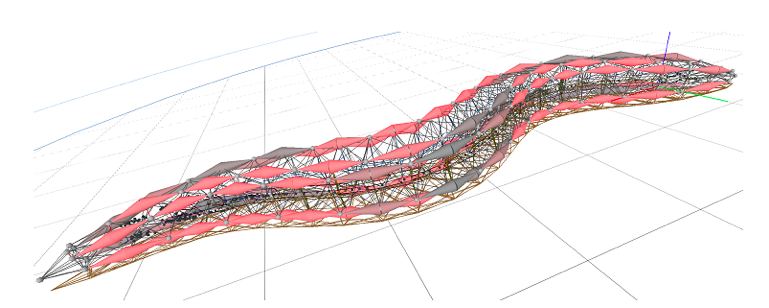
\includegraphics[scale=0.60]{cyber_elegans}
  }
  \caption{Интегрированная модель нематоды \textit{C. elegans.}}\label{fig:cyber_elegans}
\end{figure}

Несмотря на то, что довольно много биологических деталей опущено основная ценность данного прототипа заключается в доказательстве концепции того, что широкий ряд биофизических факторов - от сил, действующих на тело, до паттернов активации нейронов и движения мышц, может быть одновременно учтен и объединен в единую программную систему. На данный момент существуют более детализированные модели для двигательных систем \cite{Boyle2012} и лучшее представление для нейронов и нейросетей (NeuroML \cite {Gleeson2010} для мульти-сегментной модели) однако именно в нашей работе впервые была предложена концепция и продемонстрирован работающих прототип, объединяющий трехмерную модель тела с управляющим им фрагментом нейронной сети \cite {Palyanov2012}.

При моделирования физического тела биологического существа – от одной клетки до целого беспозвоночного организма – необходимо учитывать, каким образом в модели будут представлены механические свойства двух ее важнейших компонентов: упругого материала для внешней оболочки тела и жидкости, аппроксимирующей внутреннее содержимое тела. Части, ответственные за активное движение (такие как мышцы), также должны описываться как упругий материал, способный сокращаться под действием внешних стимулов. Жидкость также необходима для моделирования внешней среды. Трудно переоценить важность моделирования именно несжимаемой жидкости для реалистичного представления моделируемых объектов как с физической, так и с биологической точек зрения. И, наконец, необходима возможность описания и определения  взаимодействия между жидкостью и упругим материалом.

Учитывая все вышесказанное, все эти требования привели нас к тому, что в качестве базового метода моделирования механики сплошных сред был выбран метод частиц (Лагранжевый метод), как более подходящий для данной проблемы по сравнению с сеточными (Эйлеровыми) методами.  В свою очередь, это привело нас к использованию метода гидродинамики сглаженных частиц и его модификаций. Мы также представляем реализацию этого алгоритма, которая служат основой для моделирования тела нематоды \textit{C.elegans}. 3D модели как одиночной мышечной клетки, так и всего тела \textit{C.elegans} представлены в виде системы частиц и производится расчет их динамики для того, чтобы сравнить  механику мышечной клетки и модели тела с таковыми для реального организма.

Будущие результаты, полученные в этой области, могут дать новые знания о нейронных механизмах и паттернах, таких как, например, до сих пор неизвестный механизм, отвечающий за генерацию синусоидального паттерна движения. Эти результаты могут быть использованы в области дизайна искусственных нейронных сетей. Изучение возможности детальной репродукции нервной сети \textit{C. elegans} может стать  первым шагом в изучении более сложных нервных систем путем их компьютерного моделирования. Хотя часто говорят, что нервная система \textit{C. elegans} почти полностью исследована, предполагают только топологию и схему соединений между нейронами; в тоже время на более глубоких уровнях, таких как механизм преобразования сигнала и тип задействованных нейромедиаторов, нейросеть \textit{C. elegans} остается во многом неизученной.

Планируется встроить в симулятор реалистичные модели сокращения мышц \cite {Huxley1957MuscleSA}, моделирования нейронов \cite {Gleeson2010}, обеспечить работу механизмов, имитирующих сигналы, поступающие от сенсорных клеток. Для более точного моделирования механики тела необходимо помнить о капиллярных силах, влияющих на динамику и принцип движения \textit{C. elegans}. Для учета подобных эффектов необходима разработка методов, позволяющих моделировать, с достаточной степенью приближения, динамику жидкостей, эластичных тел и их взаимодействие. На определенном этапе планируется создание онлайн версии симулятора, обеспечивающей пользователям возможность максимально комфортной работы с системой, не требующей установки. Значительно более высокие требования к вычислительной мощности будут удовлетворены путем использования технологии параллельных вычислений OpenCL, позволяющей использовать все вычислительные ресурсы, имеющиеся в системе – не только центральные процессоры (CPU), но и массивы процессоров в составе мощных графических карт (GPU), таких, как NVidia Tesla, обеспечивающих прирост производительности в десятки раз по сравнению с CPU.

\section{Алгоритмы гидродинамики сглаженных частиц}\label{sec:ch1/sec3}

Рассмотрим несколько основных методов моделирования гидродинамики. Выделяют два фундаментальных способы описания математических моделей сплошной среды: сеточные методы (Эйлерово описание) и методы частиц  (Лагранжево описание) рисунок~\ref{fig:sim_class}.

\begin{figure}[ht]
  \centerfloat{
    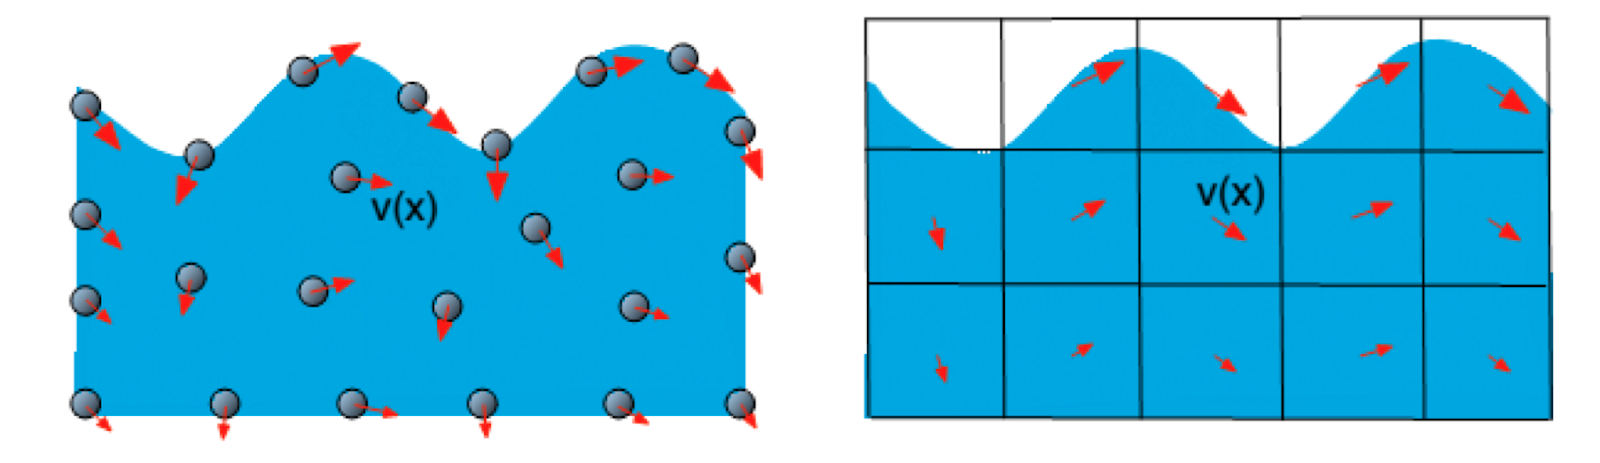
\includegraphics[scale=0.30]{sim_class}
  }
  \caption{Левый рисунок демонстрирует Лагранжево представление жидкости, жидкость представляется набором дискретных лагранжевых частиц, обладающие характеристиками необходимыми для описания траектории движения. На правом рисунке Эйлерово представление - характеристики жидкости вычисляются в фиксированных точках в пространстве, например в центре ячейки.}\label{fig:sim_class}
\end{figure}

Кроме того также выделяют смешанные методы, наиболее известным из которых является метод частиц в ячейках (PIC), разработанный в середине 50 годов Харлоу в Лос-Аламосе \cite {Harlow1963, Belocherkovsky1982, Grigoriev2000}, для моделирования плазмы. Одним из потомков PIC метода является метод сглаженных частиц (SPH - Smoothed Particle Hydrodynamics) основным отличием которого является то, что он полностью лагранжевый метод \cite{Gingold1977, Lucy1977}

Основными преимуществами метода SPH над сеточными методами являются: естественная возможность обрабатывать свободные поверхности и поверхности раздела, всплески и капли, а также взаимодействие со сложными границами и твердыми неподвижными объектами, кроме того гарантируется выполнение условия сохранение массы \cite {Müller2003, Müller2005, Keiser2005, Solenthaler2007, Solenthaler2008, Becker2007}. Изначально этот метод был предложен для решения задач, связанных с моделированием движения небесных тел, формирования звезд и галактик \cite{Gingold1977, Lucy1977}.

При моделировании методом SPH жидкость представляется набором «частиц» - дискретных элементов. Частицы характеризуются позицией в пространстве, скоростью и массой. Для представления любой физической величины  в методе SPH используется концепция интегрального представления:
\begin{equation}
\label{eq:int_rep}
A(x) = \int_{\Omega}A(x^{'})\delta (x-x^{'})dx^{'}
\end{equation}

где \(\Omega\)-некоторая область, \(dx^{'}\)-элемент объема, \(\delta (x-x^{'})\)- функция Дирака.

Если функция Дирака заменить функцией \(W\), так называемым сглаживающим ядром, с заданным радиусом сглаживания \(h\), то ~\ref{eq:int_rep} можно записать в следующем виде:
\[
A(x) = \int_{\Omega}A(x^{'})W(x-x^{'}, h)dx^{'}
\]

Сглаживающее ядро должно удовлетворять следующим условиям:
\begin{align}
\int W(x-x^{'},h)dx^{'}=1, \nonumber \\
\lim_{h\rightarrow0}W(r, h) = \delta (r). \nonumber
\end{align}

Влияние каждой частицы на свойства другой оценивается в соответствии с ее плотностью \(\rho\) и расстоянием до интересующей частицы. Математически это описывается следующим образом:
\[
A(x)=\int_{\Omega}\frac{A(x^{'})}{\rho(x^{'})}W(x-x^{'},h)dx^{'}.
\]

Заменяя интегрирование  на суммирование по соседним частицам, получаем:
\[
A(x)=\sum_{j}m_j\frac{A_j}{\rho_j}W(\left | x-x_{j} \right |,h)dx^{'}.
\]
Где \(m_j\)-масса частицы \(j\), \(A_j\) - значение величины \(A\) для частицы \(j\), \(\rho\)-плотность, связанная с частицей \(j\) и \(W\) - функция ядра. Например, плотность частицы может быть выражена как:
\[
A(x)=\sum_{j}m_j\frac{A_j}{\rho_j}W(\left | x-x_{j} \right |,h)dx^{'}=A(x)=\sum_{j}m_jW(\left | x-x_{j} \right |,h)dx^{'}.
\]
В общем случае этапы расчета смещение частицы относительно позиций на предыдущей итерации \(x(t)\), \(v(t)\) описывается следующим образом, сначала осуществляется поиск всех соседних частицы в пределах заданного радиуса сглаживания, затем рассчитываются силы, действующие на частицу, и ускорения и, наконец, вычисляется новая скорость и позиция частицы \(x(t+1)\), \(v(t+1)\).

\subsection{моделирование динамики вязкой жидкости}\label{subsec:ch1/sec4/sub1}

Модель движения несжимаемой жидкости описывается системой дифференциальных уравнений Навье-Стокса:
\begin{equation}
\label{eq:nstocs_eq1}
\rho \left ( \frac{\partial }{\partial t} + \mathbf{u} \cdot \bigtriangledown \right )\mathbf{u}=-\bigtriangledown p + \mu \bigtriangledown \cdot (\bigtriangledown \mathbf{u})+f
\end{equation}
\begin{align}
\bigtriangledown \cdot \mathbf{u} = 0 \nonumber
\end{align}
Где \(\mu\)- это коэффициент вязкости жидкости, \(f\)- сумма всех внешних сил, \(\mathbf{u}\)-скорость, \(p\)-давление. Отметить, что поскольку частицы движутся вместе с жидкостью, индивидуальная производная некоторой величины \(q\) равная полной производной \(q\frac{Dq}{Dt}=\frac{\partial q}{\partial t}\ + u \cdot \bigtriangledown q\) - это просто частная производная по времени что означает, что конвективный член в ~\ref{eq:nstocs_eq1} равен нулю \cite {Müller2003, Sedov1970}

В правой части уравнения ~\ref{eq:nstocs_eq1} описаны силы, а именно: давление \(-\bigtriangledown p\), внешние силы \(mg\) и силы вязкости \( \mu \bigtriangledown^{2}\mathbf{u} \). Уравнение движения для частицы \(i\) ~\ref{eq:nstocs_eq1} можно переписать следующим образом:
\begin{equation}
\label{eq:common_disk}
m_i\frac{D\mathbf{u}_i}{Dt}=\mathbf{F}_i^{presssure} + \mathbf{F}_i^{viscosity} + \mathbf{F}_i^{external}
\end{equation}
\begin{align}
a_i=\frac{D\mathbf{u}_i}{Dt}=\frac{F_i}{m_i} \nonumber
\end{align}
Где \(a_i\)-ускорение. Для расчета давления и сил давления используются формулы \cite {Müller2003}:
\begin{align}
p=k(\rho - \rho_0) \nonumber 
\end{align}
\begin{align}
F_{i}^{pressure}=-\sum_{j}m_j\frac{p_i+p_j}{2 \rho_j}\bigtriangledown(r_i-r_j, h) \nonumber
\end{align}
Где \(k\)– газовая постоянная Больцмана. Для расчета силы вязкости используется следующая формула \cite {Müller2003}:
\begin{align}
F_{i}^{viscosity}=-\sum_{j}m_j\frac{v_i-v_j}{2 \rho_j}\bigtriangledown^{2}(r_i-r_j, h) \nonumber
\end{align}

Для расчета плотности используется ядро \(W_{poly6}\) \cite {Müller2003}:
\[
    W_{poly6}(r,h)= \frac{315}{64\pi h^{9}}
    \begin{cases}
    (h^{2}-r^{2})^{3}, \text{если } 0 \leqslant r \leqslant  h \\
    0, \text{иначе} 
    \end{cases}
\]

Стоит отметить, что использование \(W_{poly6}\) для расчета других свойств и сил может привести к неверным результатам. Например, для вычисления давления его использование приводит к кластеризации частиц, находящихся близко друг к другу, так как градиент ядра стремится к нулю при  приближении к центру и, следовательно, отталкивающие силы исчезают \cite {Müller2003}. В работе \cite {Desbrun1996} для решения этой проблемы было предложено использовать модифицированную версию ядра \(W_{poly6}\):
\[
    W_{spiky}(r,h)= \frac{15}{\pi h^{6}}
    \begin{cases}
    (h^{2}-r^{2})^{3}, \text{если } 0 \leqslant r \leqslant  h \\
    0, \text{иначе} 
    \end{cases}
\]

Для вычисления сил вязкости ядро \(W_{poly6}\) также не подходит, так как его лапласиан почти везде отрицателен и силы, действующие между двумя близкими частицами, будут увеличивать относительную скорость частиц, что в свою очередь будет уменьшать стабильность системы \cite {Müller2003}.  Для вычисления сил вязкости используется ядро:
\[
    W_{viscosity}(r,h)= \frac{15}{2\pi h^{3}}
    \begin{cases}
    -\frac{r^{3}}{2h^{3}}+\frac{r^{2}}{h^{2}} \frac{r}{2h} - 1, \text{если } 0 \leqslant r \leqslant  h \\
    0, \text{иначе} 
    \end{cases}
\]
лапласиан, которого положителен везде.

\begin{figure}[ht]
  \centerfloat{
    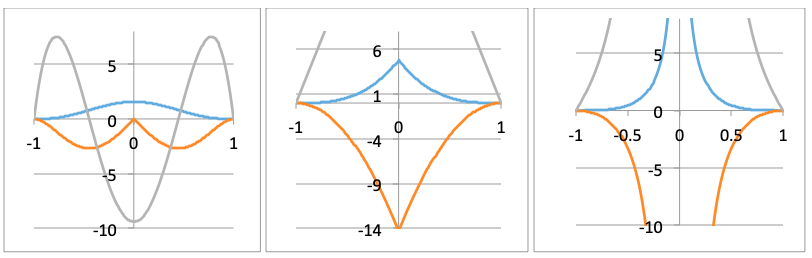
\includegraphics[scale=0.50]{ker_kind}
  }
  \caption{Сглаживающие ядра \(W_{poly6}\), \(W_{spiky}\), \(W_{viscosity}\) слева направо, представленные в работе \cite {Müller2003}. Синей линией показаны ядра, красной градиенты и зеленой лапласианы, соответственно.}\label{fig:ker_kind}
\end{figure}

Базовый алгоритм SPH не предполагает не сжимаемости моделируемой жидкости, что является одним из ключевых недостатков метода, так как подобные свойства довольно сложно воспроизвести в не сеточном методе. Однако для решения этой проблемы было предложено несколько модификаций стандартного метода SPH: WSPH \cite {Becker2007}, ISPH \cite {Shao2003, CUMMINS1999584} и PCI SPH \cite {Solenthaler2009}. Метод WSPH для обеспечения небольших колебаний плотности, при вычислении давления используется параметр жесткости \(k=c_{s}^2\) где \(c_{s}\) - скорость звука в веществе. Параметр \(k\) подобран таким образом, что скорости звука достаточно для того, чтобы сдерживать флуктуации плотности на достаточно малом уровне ~1\%  \cite {Solenthaler2009} согласно \cite {Monaghan2005}
\[
\frac{\left | \delta \rho \right |}{\rho_{0}}=\frac{\left | \boldsymbol{u} \right |^2}{c_{s}^2},
\]
где \(\boldsymbol{u}\) – максимальная скорость жидкости, \(\left | \delta \rho \right |\) и \(\rho_{0}\) плотность \(\frac{\left | \delta \rho \right |}{\rho_{0}} \sim \eta \) и, следовательно, \(k=c_{s}^{2}=\frac{\left | \delta \boldsymbol{u} \right |^{2}}{\eta}\). Однако, необходимо не  забывать о стабильности системы и выполнение критерия Куранта — Фридрихса — Леви \cite {Courant1967}
\[
\Delta t_{c} \leq \alpha \frac{h}{c}
\]
где \(h\) - радиус сглаживания, \(\alpha \sim 0.4\), \( c \)-скорость звука, как можно заметить неравенство будет выполняться только в случае достаточно маленького временного шага.

ISPH использует метод проекций, введенный в работах \cite {Temam1968, Chorin1968}: скорости на каждом шаге проектируются в бездивергентное векторное поле:
\[
\boldsymbol{div}\vec{u}=0
\]
решается уравнение Пуассона:
\begin{equation}
\label{eq:puasson}
\bigtriangledown^{2} p^{n+1}=\frac{\rho}{\Delta t}\bigtriangledown \cdot \boldsymbol{u}^{*}
\end{equation}
где \(\boldsymbol{u}^{*}\) промежуточное значение скорости, полученное из \(\boldsymbol{u}^{n}\) ( \(n\)– номер итерации ) путем подстановки \(\boldsymbol{u}^{n}\) в уравнение движения ~\ref{eq:common_disk}, игнорируя при этом градиент давления:
\[
m_i\frac{\textbf{u}_{i}^{*} -\textbf{u}_{i}^{n}}{\Delta t} = \mathbf{F}_i^{viscosity} + \mathbf{F}_i^{external},
\]
Вычислив значение давление на шаге \( n+1 \), вычисляется новое значение скорости:
\[
\textbf{u}^{n+1}=\textbf{u}^{*}+\frac{\Delta t}{\rho}\bigtriangledown p^{n+1}.
\]

Таким образом, гарантируется выполнение свойства несжимаемости на следующей итерации. Этот метод стабилен при большом временном шаге, но требует большое количество вычислений на одну итерацию.
При выборе оптимального варианта мы ориентировались как на минимизацию вычислительных затрат в единицу времени и возможность работы симуляции при относительно большом временном шаге, так и на приемлемый уровень точности получаемого решения. Всем этим требованиям отвечает метод PCI SPH (predictor-corrector incompressible smoothing particle hydrodynamics) \cite {Solenthaler2009}, в котором несжимаемость жидкости обеспечивается путем использования схемы “предиктор-корректор” для определения давления в точках пространства, занимаемых частицами. Для этого информация о флуктуациях плотности активно распространяется через жидкость и значения давления обновляются пока значения плотности во всей системе не станет удовлетворительными. При таком подходе исчезает необходимость решать уравнение Пуассона для давления ~\ref{eq:puasson} требующая значительных вычислительных затрат, и в то же время остается возможность корректной работы симуляции с большим временным шагом - более чем на порядок большем чем при использовании метода WSPH. На каждой итерации для всех частиц рассчитываются позиции и скорости \(x_{i}^{*}(t+\Delta t)\), \(v_{i}^{*}(t+\Delta t)\) исходя из \(x_{i}^{*}(t)\), \(v_{i}^{*}(t)\). Затем рассчитывается отклонение плотности:
\[
\rho_{err_{j}}^{*}(t+\Delta t)=\rho_{i}^{*}(t+\Delta t) - \rho_{0},
\]
где \(\rho_{i}^{*}(t+\Delta t) + \rho_{0}=\sum_{j} m_{j} W(x_{ij}^{*}, h) \), \(x_{ij}^{*}=x_{i}^{*}(t + \Delta t)-x_{j}^{*}(t + \Delta t)\),
которое используется для коррекции давления и, как следствие, сил давления:
\[
p_{i}(t) += \delta \rho_{err_{i}}^{*}(t+\Delta t),
\]
где \(\delta\) - рассчитано заранее значение, которое определяется по следующей формуле:
\[
\delta=\frac{-1}{\beta(-\sum_{j}\Delta W_{ij}^{0} \cdot \sum_{j}\Delta W_{ij}^{0}-\sum_{j}\Delta W_{ij}^{0} \cdot \Delta W_{ij}^{0})} ,
\]
\[
\beta=2(\frac{m_i \cdot \Delta t}{\rho_0})^2 ,
\]
\(W_{ij}^{0}=W(x_{ij}^{0})\), \(x_{ij}^{0}\) - это начальная позиция прототипной частицы. И наконец, силы давления рассчитываются следующим образом:
\[
F_{i}^{p}(t)=-m_i \sum_{j} m_j \left ( \frac{p_i(t)}{(\rho_{i}^{*})^2} + \frac{p_j(t)}{(\rho_{j}^{*})^2} \right )\Delta W(x_{ij}, h)
\]
Эта процедура повторяется пока \( max( \rho_{err_{i}}^{*} ) \) будет не больше определенного пользователем порогового значения (обычно 1\% - 3\% от характерной величины , для воды 1000 кг/м\textsuperscript{2}). Предлагается, проделывать не более трех итераций, чтобы ограничить колебание давления.

Стоит также отметить, что при смещении частиц во временные позиции список соседей, вообще говоря, может измениться. Но для повышения производительности алгоритма предполагается использовать старое множество соседей (что почти всегда выполняется; даже если есть несоответствия, то, как правило, на границе расстояния сглаживания, что дает минимальный вклад в общую величину) и только пересчитывать расстояния. Это приближение приводит к небольшим ошибкам в оценках плотности и давления, которыми можно пренебречь \cite{Solenthaler2009}. Схема алгоритма PCI SPH продемонстрирована ниже схема \ref{algo:pcisph}
\begin{algorithm}
\label{algo:pcisph}
\SetAlgoLined
\SetKwFunction{Union}{Union}\SetKwFunction{FindNeighbour}{FindNeighbour}\SetKwFunction{ComputeForce}{ComputeForce}\SetKwFunction{PredictVelocity}{PredictVelocity}\SetKwFunction{PredictPosition}{PredictPosition}\SetKwFunction{PredictDensity}{PredictDensity}\SetKwFunction{PredictDensityVariation}{PredictDensityVariation}\SetKwFunction{ComputeVelocity}{ComputeVelocity}\SetKwFunction{ComputePosition}{ComputePosition}
\SetKwInOut{Input}{input}\SetKwInOut{Output}{output}
\Input{$\mathcal P$ array of particles}

\ForEach{$p \in \mathcal P$}
{
${N_{p}} \leftarrow$ \FindNeighbour{$p, \mathcal P $}\;
}
\ForEach{$ p \in \mathcal P $}{
$F^{v,g,ext}(t) \leftarrow$ \ComputeForce{$p, \mathcal P $}\;
$p(t) \leftarrow 0.0$\;
$F^{p}(t) \leftarrow 0.0$\;
 }
 \While{$\rho_{err}^{*}(t+1)>\eta || (iter < minIterations)$}{
 \ForEach{$p \in \mathcal P$}{
    ${v_{p}^{*}(t+1)} \leftarrow$ \PredictVelocity{$p$}\;
    ${x_{p}^{*}(t+1)} \leftarrow$ \PredictPosition{$p$}\;
 }
 \ForEach{$p \in \mathcal P$}{
    $\rho_{err}^{*}(t+1) \leftarrow$ \PredictDensity{$\mathcal{P}$}\;
    $\rho_{err}^{*}(t+1) \leftarrow$ \PredictDensityVariation{$\mathcal{P}$}\;
    $p_{p}(t) += f(\rho_{err}^{*}(t+1))$\;
 }
 \ForEach{$p \in \mathcal P$}{
    $F^{p}(t) \leftarrow$ \ComputeForce{$p, \mathcal P $}\;
 }
 }
 \ForEach{$p \in \mathcal P$}{
    ${v_{p}(t+1)} \leftarrow$ \ComputeVelocity{$p$}\;
    ${x_{p}(t+1)} \leftarrow$ \ComputePosition{$p$}\;
 }
\caption{Схема алгоритма PCI SPH}
\end{algorithm}

\subsection{Неподвижные объекты и границы}\label{subsec:ch1/sec4/sub2}

Для обработки взаимодействия частиц с границей было предложено несколько методов, зачастую использующихся в различных реализациях PCI SPH:

\begin{itemize}
\item основанный на использование корректирующих сил \cite {Müller2004}
\item основанный на корректировки сил и позиций \cite {Becker2009}
\end{itemize}

Основным недостатком вышеуказанных методов является сложность обработки взаимодействия частиц с границей сложной геометрии. Одним из возможных решений данной проблемы является метод, предложенный в работе  \cite {Ihmsen2010}, основной особенностью данного подхода является использование граничных частиц. Подобная техника позволяет корректно обрабатывать контакт с границей, а кроме того, дает возможность создавать границы разных форм, не опасаясь залипания частиц. Граница представляется в виде набора граничных частиц, расположенных в узлах решетки с заданным шагом; для каждой такой частицы используются те же характеристики, что и для обычных частиц, но, в отличие от них, граничные частицы неподвижны рисунок \ref{fig:boundary}
\begin{figure}[ht]
  \centerfloat{
    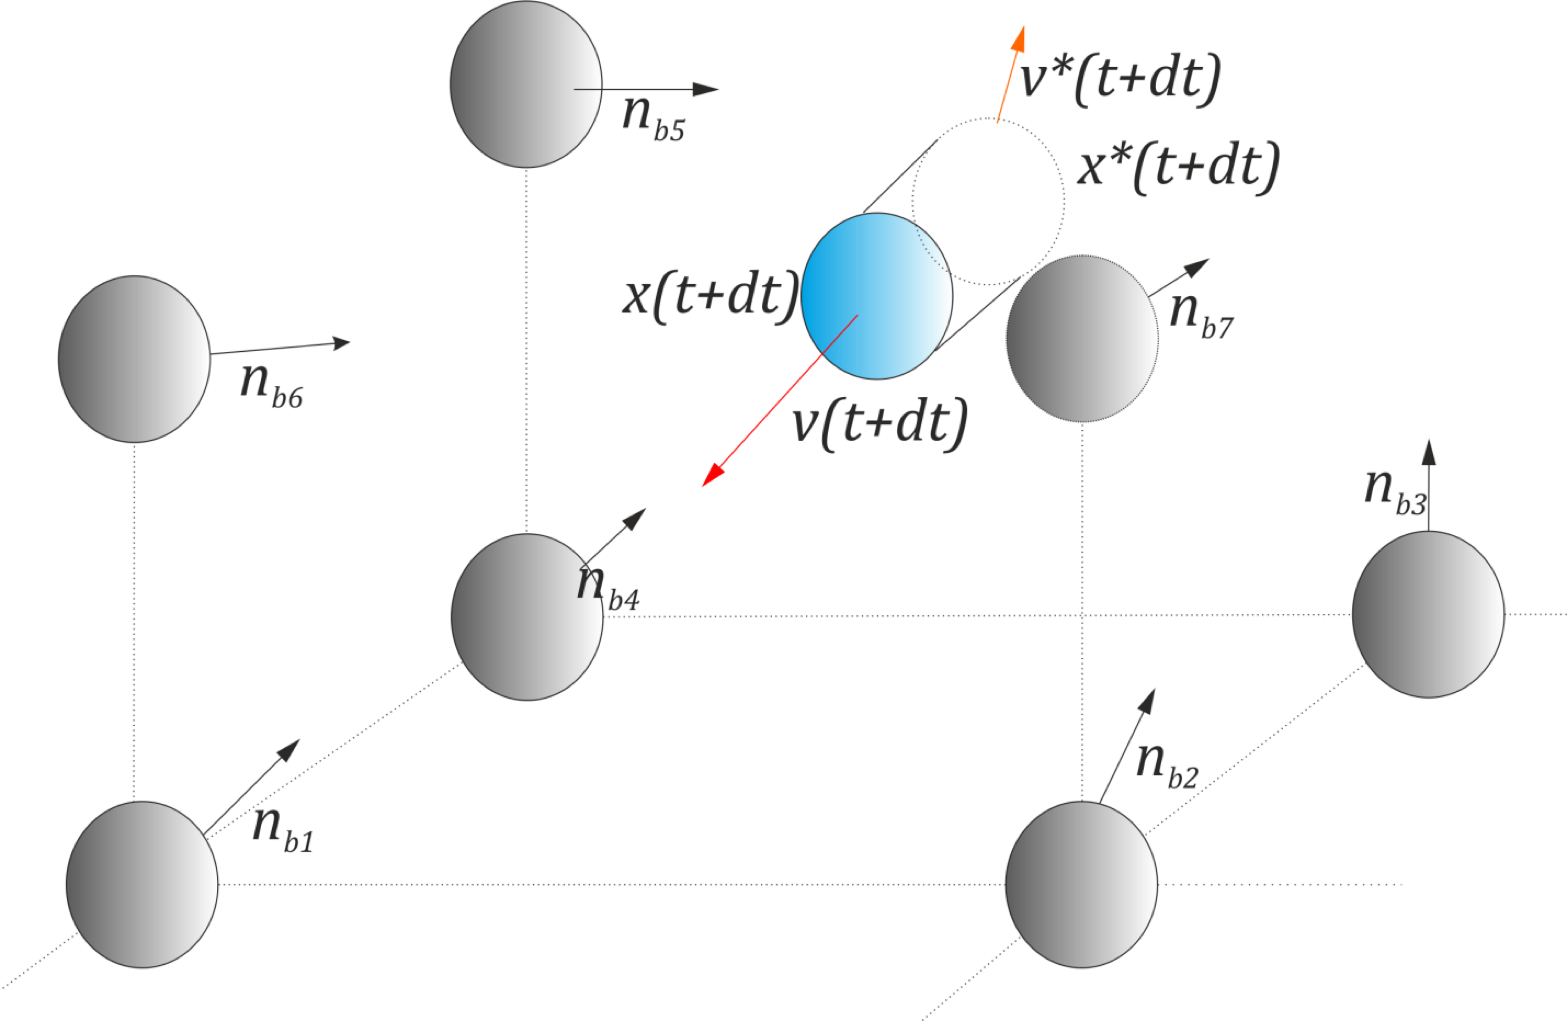
\includegraphics[scale=0.20]{boundary}
  }
  \caption{Взаимодействие граничных частиц с частицей жидкости, залетевшей в один из углов ограничивающего объема. Красной стрелкой показано направление и величина скорости \(v(t+dt)\), черными стрелками показаны нормали, исходящие из граничных частиц, представленные серыми сферами. Оранжевой стрелкой и прозрачной сферой обозначено направление скорости и положение частицы жидкости \(v^{*}(t+dt)\) и \(x^{*}(t+dt)\) после взаимодействия с границей.}
\label{fig:boundary}
\end{figure}

Взаимодействие между частицами и граничными частицами обрабатывается следующим образом, для каждой частицы, которая имеет в списке соседей граничные частицы, считаются граничные силы \(F^{boundary}\), которые влияют на распределение плотности жидкости. Отметим, однако, что частица попадает в поле действия граничных сил, только в том случае если \(\left \| x_i - x_{boundary}  \right \| \leq \frac{h}{2}=r_0\) где \(x_i\) – позиция \(i\)-й частицы \(x_{boundary}\) – позиция граничной частицы. Согласно описываемой модели, граничные частицы влияют на координаты и скорость \(i\)-й частицы следующим образом:
\[
v_{i}^{*}(t + \Delta t) = \epsilon \left [ v_{i}(t+\Delta t) \right ]_{t}
\]
где, \(\left [ v_{i}(t+\Delta t) \right ]_{t} = v_{i}(t+\Delta t) - \left [ v_{i}(t+\Delta t) \right ]_{n}\), \(\left [ v_{i}(t+\Delta t) \right ] = (v_{i}(t_i + \Delta t)\cdot n_b) \cdot n_b \) и \(n_b\) - нормаль, \( \epsilon \in \left [ 0, 1 \right ] \). При этом позиция частицы корректируется в соответствии с информацией о множество частиц граница, которые попадают окрестность:
\[
x_{i}^{*}(t+\Delta t) = x_{i}(t+\Delta t) + \frac{1}{\sum_{b}w_{ib}^{c}}\sum_{b}w_{ib}^{c}(r_0 - \left \| x_{ib} \right \|)\frac{n_{i}^{c}}{\left \| n_{i}^{c} \right \|}
\]
где \(n_{i}^{c}=\sum_{b}w_{ib}^{c}n_b\), \(n_{b}\) - нормаль к границе, направленная из граничной частицы, если граничная частица находится на пересечении нескольких граней ограничивающего объема, то нормаль из этой частицы считается как сумма нормалей этих граней, \(w_{ib}^{c}=max(0, \frac{r_0 - \left \| x_{ib}^{*} \right \|}{r_0})\), \(\left \| x_{ib} \right \| = \left \| x_{i}(t+\Delta t) - x_{b} \right \|\).
           % Глава 1
\chapter{Вычисление в гетерогенных вычислительных средах}\label{ch:ch2}

\section{Проблемы распараллеливание алгоритмов класса SPH на гетерогенных вычисленных системах с разделяемой памятью}\label{sec:ch2/sec1}

В классической задаче \(N\) тел при расчете силы, действующей на любой объект, необходимо учитывать влияние на этот объект всех тел в системе, из чего следует, что для таких алгоритмов характерна квадратичная асимптотическая сложность \(O(N^2)\). Это одна из ключевых проблем любой численной модели на основе частиц, так как при существовании требования большей детализации возникает необходимость использовать большого количества частиц. В свою очередь для вычисления следующего состояния системы для каждой частицы важно знать физические параметры любой другой частицы.

Комбинированный метод PIC (PIC – particle in cell) \cite{Harlow1963, Grigoriev2000, Belocherkovsky1982} и его модификации \cite{Belocherkovsky1982}, предполагают, что сплошная среда описывается как частицами так и фиксированной сеткой. При этом частицы несут в себе информацию лишь о массе в то время как информация об флуктуациях физических величин в системе распространяется через фиксированные узлы сетки.
Таким образом для синхронизации параллельных вычислений на различных узлах кластера или устройствах одного узла достаточно лишь своевременного обновления значений в узлах сетки и информацию о количестве частиц в ячейки.

В то же время полностью Лагранжевые алгоритмы такие как SPH система координат связана с движением жидкости в пространстве (сетка движется вместе с жидкостью) и отвечает фиксированным точкам в среде. Таким образом сплошная среда представляется как дискретное множество частиц. Информация в среде передается исключительно через частицы, что делает трудным распараллеливание вычислений на разных физических узлах кластера или между GPU (графический сопроцессор) в пределах одного вычислительного узла или устройства. Для численных моделей основанных на системе частиц, не смотря на то, что каждый метод хорошо распараллеливаются по данным, представляется довольно сложным распределение вычислений на системах с не общей памятью - такие как узлы кластера общающиеся по сети или различные вычислительные устройства в рамках одной машины, но независимыми модулями оперативной памяти (GPU). Это в частности обусловлено тем,  что частицы динамичны и не привязаны к определенным позициям, как узлы расчетных сеток. Тем ни менее, в работах \cite {Dominguez2013, Verma2017, Verma2018} предложены попытки преодолеть этот недостаток за счет логичного разделения моделируемого пространства на не пересекающиеся статичные или динамичные подпространства - домены. Таким образом частицы можно кластеризовать по пространственному признаку, в зависимости от текущей позиции. При этом подразумевается, что каждый домен обрабатывается отдельным  устройством - вычислителем. В нашей интерпретации метода PCI SPH мы также основывались на этом подходе ниже в таблице \ref{tab:algocmp1} представлено сравнение между нашим и аналогичными подходами.

\begin{table} [htbp]% Пример записи таблицы с номером, но без отображаемого наименования
  \centering
  \begin{threeparttable}% выравнивание подписи по границам таблицы
    \caption{Реализации подходов распараллеливания методов частиц на нескольких устройствах}%
    \label{tab:algocmp1}%
    \begin{SingleSpace}
      \begin{tabular}{| c | c | c | c |}
        \hline
        Источник              & \thead{Технология \(||\) вычислений} & Алгоритм & \thead{Доступность (Open source) } \\ \hline
        \cite {Dominguez2013} & CUDA + MPI                           & SPH      & -                                  \\ \hline
        \cite {Verma2017}     & CUDA                                 & SPH      & -                                  \\ \hline
        \cite {Verma2018}     & CUDA                                 & PCI SPH  & -                                  \\ \hline
        Sibernetic            & OpenCL                               & PCI SPH  & +                                  \\ \hline
      \end{tabular}%
    \end{SingleSpace}
  \end{threeparttable}
\end{table}

\section{Алгоритм поиска соседей}\label{sec:ch2/sect2}
Наряду с неэффективным методом перебора всех частиц были предложены другие алгоритмы, базирующиеся на пространственном делении всей области на ячейки \cite {Teschner2003, Kipfer2006, Keiser2006, Cohen1995}. Подобные алгоритмы предполагают, что можно пренебречь незначительным влиянием частиц, находящихся на расстоянии, превышающем определенную длину сглаживания рисунок ~\ref{fig:ns_1}.
\begin{figure}[ht]
  \centerfloat{
    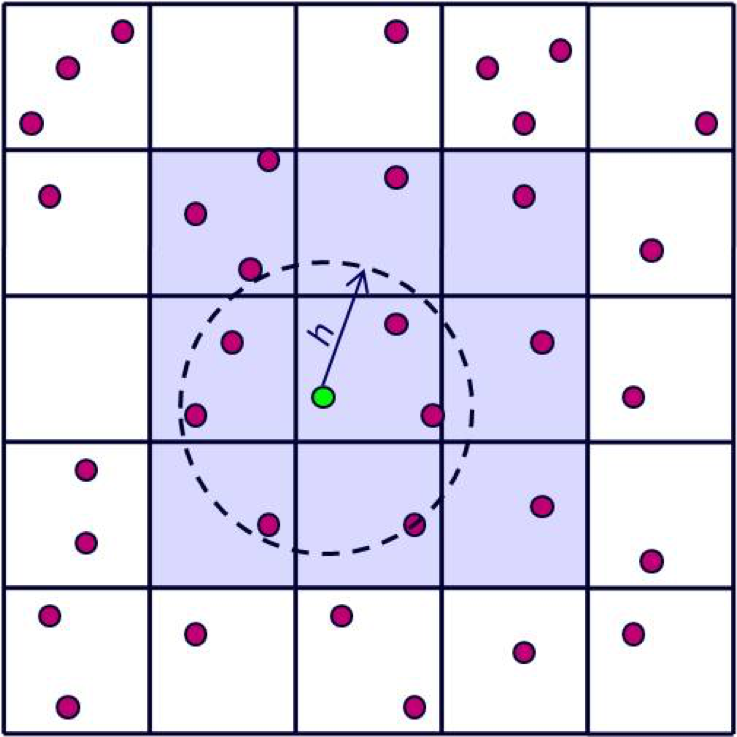
\includegraphics[scale=0.30]{ns_1}
  }
  \caption{Поиск соседей в ближайших смежных ячейках.
  }\label{fig:ns_1}
\end{figure}
Это позволяет свести сложность алгоритма к \(O(M \cdot N)\), где \(M < N\).

Использование подобных методов позволяет в целом сократить количество вычислений, однако необходимо помнить, что, наряду с остальными задачами, возникает проблема, связанная обновлением списка соседей для каждой частицы каждую итерацию. «Поиск соседей» является одной из самых важных стадий алгоритма и одной из самых трудоемких операций. Как правило, она занимает порядка 30\% времени работы симуляции за один шаг. Существует два способа кластеризации частиц в пространстве в зависимости от их текущих позиций - KD-дерево и пространственный хеш. Основным недостатком KD-деревьев является необходимость перестраивать их на каждой итерации в связи с тем, что система динамична таблица \ref{tab:algoNS1}.

\begin{table} [htbp]% Пример записи таблицы с номером, но без отображаемого наименования
  \centering
  \begin{threeparttable}% выравнивание подписи по границам таблицы
    \caption{ Алгоритмы поиска списка соседей. }%
    \label{tab:algoNS1}%
    \begin{SingleSpace}
      \begin{tabular}{| c | c | c |}
        \hline
        Название                     & +                                     & -                                      \\ \hline
        Перебор                      & Простота реализации                   & {\makecell { Aсимптотическая сложность \\ \( O(n^2)\) }} \\ \hline
        KD-дерево                    & {\makecell {Быстро и эффективно можно                                          \\
        находить ближайших соседей}} & {\makecell {Необходимо перестраивать                                           \\ дерево на каждой итерации \\
        (система динамична)}}                                                                                         \\ \hline
        Хеш функция                  & {\makecell {Быстро и эффективно                                                \\ можно находить \\ ближайших соседей }} & {\makecell {Сортировка массива \\ частиц на \\ каждой итерации }} \\ \hline
      \end{tabular}%
    \end{SingleSpace}
  \end{threeparttable}
\end{table}

Алгоритм разбит на несколько стадий, каждая из которых описана ниже. На начальном этапе пространство делится на равные ячейки, ширина, длина и глубина которых равна \(2h\) ( \(h\)радиус сглаживания); инициализируются специальные списки, в которых будет храниться информация о соседних частицах. Для алгоритма PCI SPH верно следующее утверждение: количество частиц в любом объеме ограничено константой. В силу того, что алгоритм PCI SPH моделирует несжимаемую жидкость можно утверждать, что количество частиц в в любом объеме не должно  превосходить некоторое число, что бы поддерживалось условие не сжимаемости. То есть плотность моделируемой не должно превосходить стандартную плотность более чем на заданный процент. Отсюда можно оценить максимальное количество частиц в каждой пространственной ячейки исходя из пространственных параметров ячейки. По нашим оценкам, для реализации алгоритма PCI SPH \(M\) не превосходит 1220 в силу не сжимаемости жидкости.

На втором этапе для каждой частицы, вычисляется пространственный индекс ячейки, в которой она находится в текущий момент времени \cite {Teschner2003} полученный индекс помещается в массив \(particleIndex\).  Индекс зависит от позиции частицы и вычисляется следующим образом:
\[
  cell(x,y,z,h) = \left( \left \lfloor \frac{x - x_{min}}{2h} \right \rfloor, \left \lfloor \frac{y - y_{min}}{2h} \right \rfloor, \left \lfloor \frac{z - z_{min}}{2h} \right \rfloor \right ) = (i,j,k)
\]
\[
  cellID = j + k \cdot gridCellY + i \cdot gridCellZ \cdot gridCellY
\]

Заполненный массив \(particleIndex\) сортируется по ячейкам алгоритмом быстрой сортировки рисунок ~\ref{fig:ns_2}, в соответствии с этим списком сортируются позиции и скорости, соответствующие значения помещаются в специальные временные списки.
\begin{figure}[ht]
  \centerfloat{
    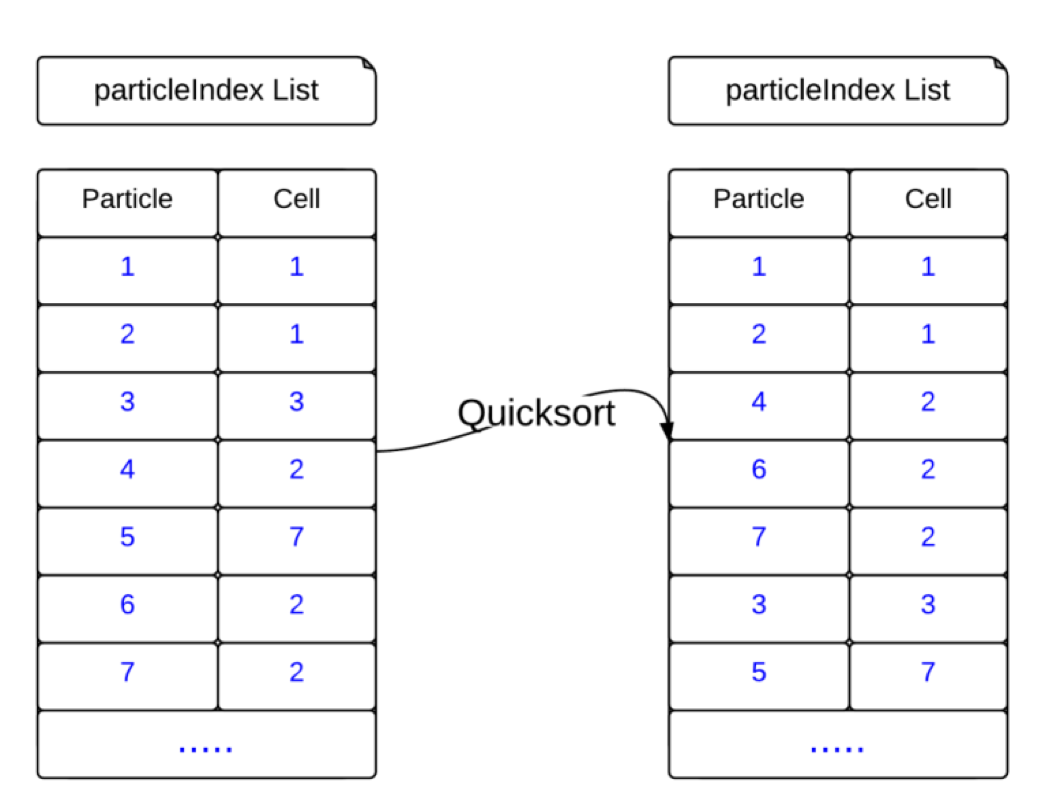
\includegraphics[scale=0.30]{ns_2}
  }
  \caption{Список \(particleIndex\) после сортировки.}
  \label{fig:ns_2}
\end{figure}

Все это позволяет быстро извлекать значения скоростей и позиции частиц, лежащих в определенной ячейке. Однако после сортировки позиции в списке \(particleIndex\) не соответствуют списку позиций частиц, и довольно проблематично отслеживать изменения свойств одной определенной частицы. Для решения этой проблемы был введен список \(particleIndexBack\), который дублирует список \(particleIndex\) до сортировки рисунок ~\ref{fig:ns_3}, это позволяет, в том числе, эффективно отлаживать приложение в условиях параллельного программирования.
\begin{figure}[ht]
  \centerfloat{
    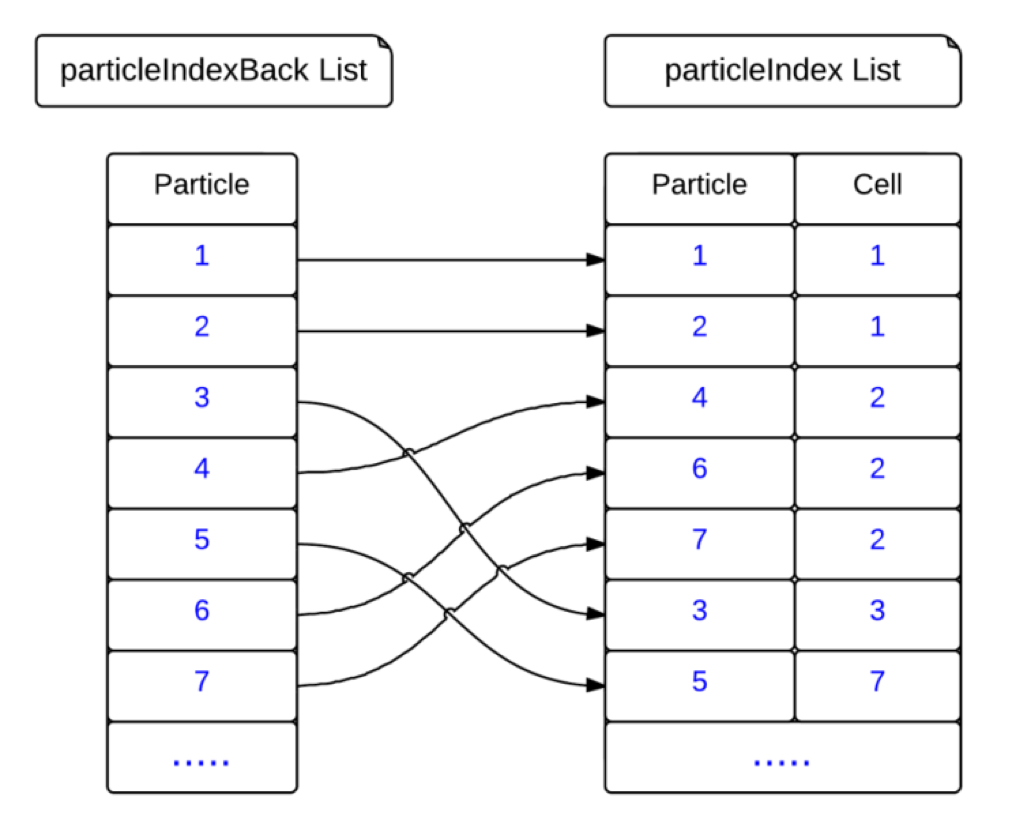
\includegraphics[scale=0.30]{ns_3}
  }
  \caption{Связь между списком \(particleIndexBack\) и \(particleIndex\).}
  \label{fig:ns_3}
\end{figure}

На третьей стадии алгоритма, при непосредственном поиске соседей, для каждой частицы среди потенциальных соседних частиц (частиц которые находятся не дальше чем \(h\)) необходимо отобрать не более 32 ближайших. Поиск потенциальных соседей в первую очередь проходит в «домашней» ячейке (ячейка, в которой на данный момент находится частица), затем вычисляется положение частицы в ячейке, для этого ячейка разбивается на 8 равных пространственных фрагментов с длиной грани равной радиусу сглаживания рисунок ~\ref{fig:ns_4}.
\begin{figure}[ht]
  \centerfloat{
    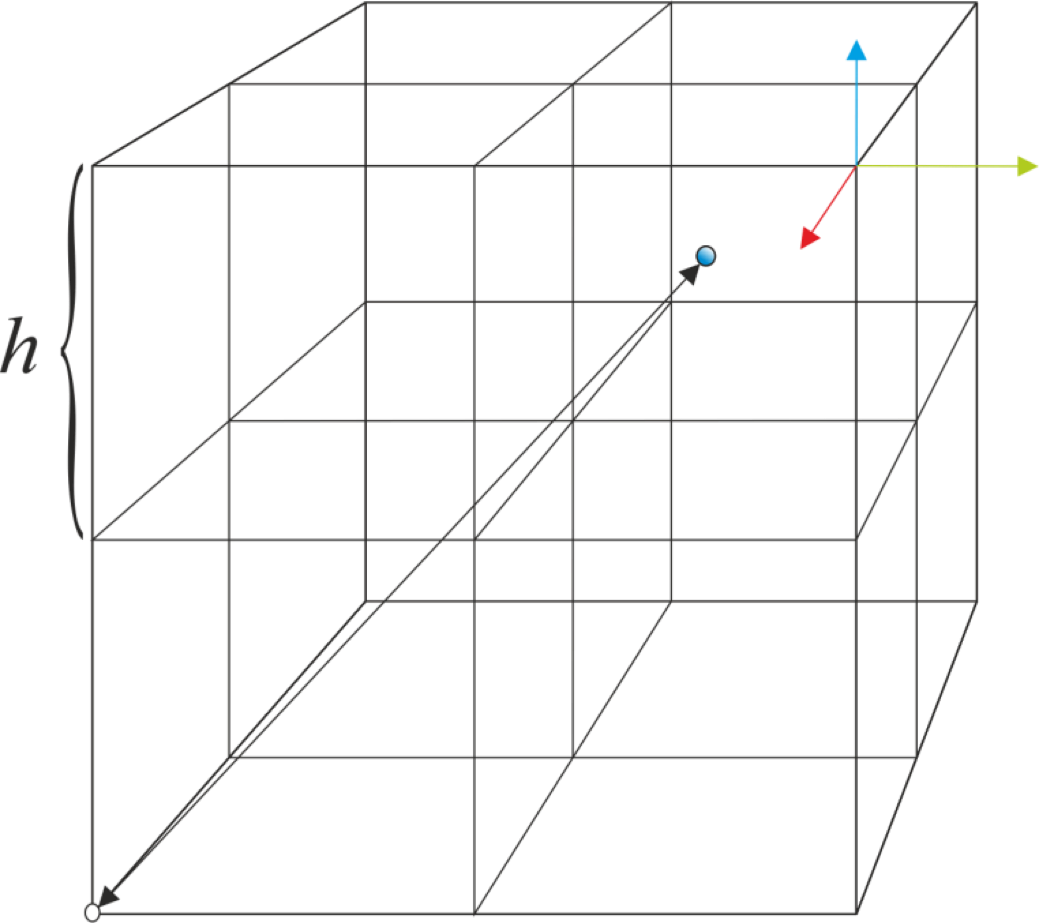
\includegraphics[scale=0.20]{ns_4}
  }
  \caption{Разбиение ячейки на 8 равных фрагментов.}
  \label{fig:ns_4}
\end{figure}

Поиск оставшихся «потенциальных» соседей проходит в семи смежных для пространственного фрагмента ячейках. Это позволяет избежать вычислений, связанных с рассмотрением частиц, лежащих заведомо дальше, чем радиус сглаживания.

Формально можно представить список соседей как множество индексов частиц \(N_{i,h}=\left \{ j|\left | r_i-r_j \right | \leqslant h \right \}\). Для того чтобы отобрать наиболее близкие частицы, сначала необходимо выяснить на каком минимальном расстоянии \(h_min \leq  h\) находится удовлетворяющее нас количество ближайших частиц \(N_{i,h_{min}}=\left \{ j|\left | r_i-r_j \right | \leqslant h \right\} \subseteq N_{i,h}\). Для этого анализируется множество \(Nd_i=\left \{ k_{i,j}|k_{i,j}=\left | N_{i,\frac{h\cdot j}{s}} \right | - \left | N_{i,\frac{h\cdot (j-1)}{s}} \right |, j\in [1,...,s] \right \}\), где \(s=30\), и для частицы \(i\) получает \(h_{min}=\frac{(j+1)\cdot h}{s} |  j = \max_{1\leq c\leq s}\left ( c|\sum_{l=1}^{c} k_{i,l} \right )\leq NeighbourCount, k_{i,l} \in Nd_j\) \(NeighbourCount=32\) ~\ref{fig:ns_5}.
\begin{figure}[ht]
  \centerfloat{
    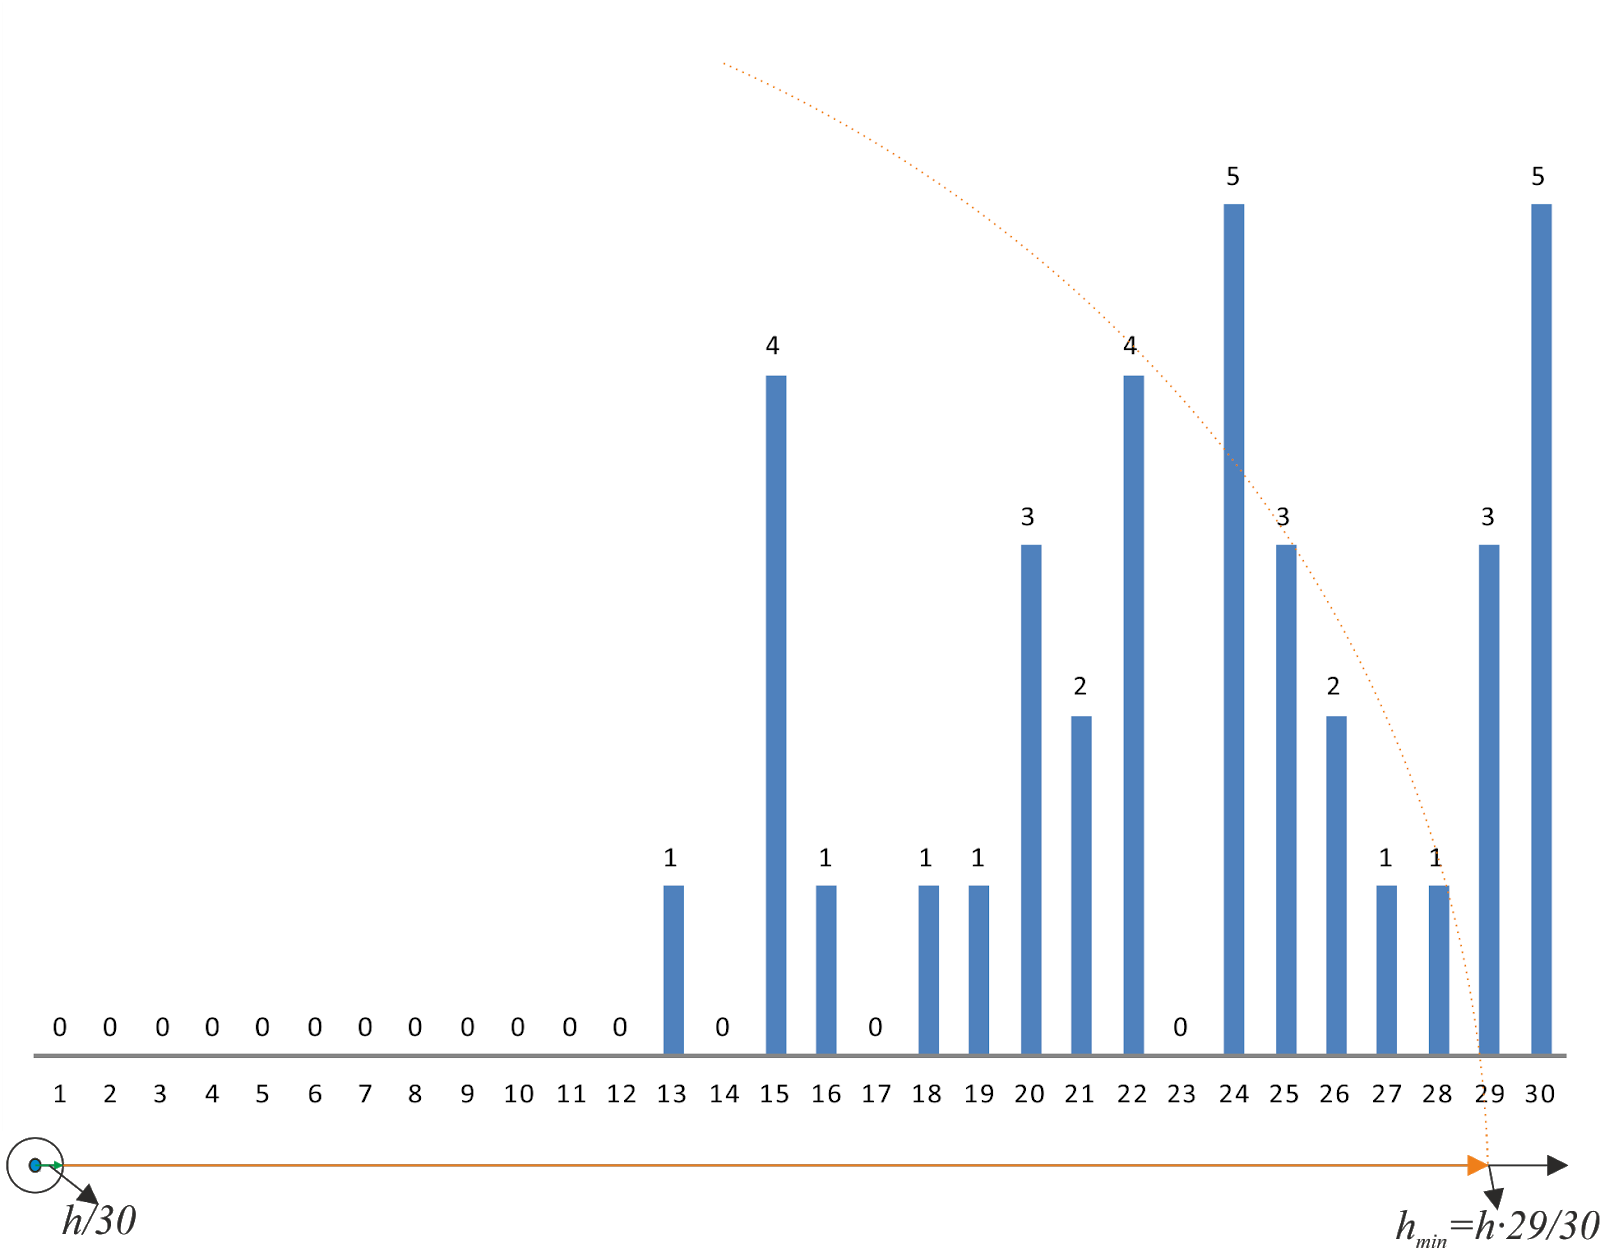
\includegraphics[scale=0.20]{ns_5}
  }
  \caption{Иллюстрация принципа выбора минимального радиуса. Гистограмма распределения расстояний от данной частицы \(i\) до соседних частиц. На данном примере достаточное количество соседних частиц, а именно 32, находится внутри сферы радиусом.}
  \label{fig:ns_5}
\end{figure}
Ниже приведена схема алгоритма поиска соседей ~\ref{algo:ns}.

\begin{algorithm}[H]
  \label{algo:ns}
  \SetAlgoLined
  \SetKwFunction{Neighbour}{Neighbour}
  \SetKwFunction{PutNeighbour}{PutNeighbour}
  \SetKwFunction{SearchParticlesForCell}{PutNeighbour}
  \SetKwFunction{Dist}{Dist}
  \SetKwInOut{Input}{input}\SetKwInOut{Output}{output}
  \Input{$\mathcal P$ множество частиц}
  \Input{$\mathcal N_{map}$ список списков всех соседей для каждой частицы}
  \Input{$\mathcal C$ список пространственных ячеек }
  \ForEach{$p \in \mathcal P$}
  {
    $r_s  \leftarrow 30 $\;
    $array[1...r_s]\, r_d \leftarrow [0...0]$\;
    $searchMode \leftarrow false$\;
    $h_{min} \leftarrow h$\;
    \textbf{search}: \\
    \ForEach{$c \in \mathcal C$}
    {
      $P_c \leftarrow \left \{ \mathcal P_c \subseteq \mathcal P| \forall p_{i}\in \mathcal P_{c} \Rightarrow p_{i}.cellID = c \right \} $\;
      \SearchParticlesForCell{$\mathcal N_{map}$[p], $h_min$, $searchMode$}\;
      $searchMode \leftarrow true$\;
      \If{$searchMode == true$}{
        $n_{c} \leftarrow 0$\;
        \ForEach{$j \in [1...r_{s}]$}{
          $n_{c} \leftarrow n_c + r_{d}[j]$\;
          \If{$n_c > 32$}{
            $h_{min} \leftarrow (j-1)\cdot \frac{h}{r_s}$ \;
            \textbf{goto search}\;
          }
        }
      }
    }
  }
  \caption{Схема алгоритма поиска соседей}
\end{algorithm}

Процедура поиска множетва частиц в пространственной ячейке \(c\) описана в схеме ~\ref{algo:ns_c}.

\begin{algorithm}[H]
  \label{algo:ns_c}
  \SetAlgoLined
  \SetKwFunction{Neighbour}{Neighbour}
  \SetKwFunction{PutNeighbour}{PutNeighbour}
  \SetKwFunction{Dist}{Dist}
  \SetKwInOut{Input}{input}\SetKwInOut{Output}{output}
  \Input{$\mathcal P_c$ множество частиц для ячейки c}
  \Input{$\mathcal N_{map}$ список списков всех соседей для каждой частицы}
  \Input{$h_{min}$ радиус}
  \Input{$ searchMode$ режим поиска/заполенния}
  $r_s  \leftarrow 30 $\;
  $h_{min} = h$\;
  \ForEach{$p_{n} \in \mathcal P_c = \left \{ \mathcal P_c \subseteq \mathcal P| \forall p_{i}\in \mathcal P_{c} \Rightarrow p_{i}.cellID = c \right \} $}
  {
    d = \Dist($p$,$p_{n}$)\;
    \If{$d \leq h_{min}$}{
      \eIf{$searchMode \neq true$} {
        $r_{j} \leftarrow \left [ d \cdot \frac{r_{s}}{h} \right ] $\;
        $r_{d}[r_{j}] \leftarrow r_{d}[r_{j}] + 1$\;
      }
      {
        $neighbour \leftarrow Neighbour(p_{i}, d)$ \;
        \PutNeighbour{$\mathcal N_{map}$[p], $neighbour$}\;
      }
    }
  }
  \caption{Схема алгоритма поиска частиц в окресности для заданной ячейке.}
\end{algorithm}

Функция \( Dist \) - расчитавает растояние между частицами как растояние Евклида.

\section{Алгоритм распределения зависимых данных по разным вычислительным устройствам}\label{sec:ch2/sec3}
Основная идея алгоритма заключается в распределении данных между независимыми вычислительными устройствами-вычислитель. Независимость вычислителя обуславливается его изолированностью относительно вычислительных мошностей и памяти. Рапределение производится таким образом, чтобы обеспечить каждую частицу, обрабатываемую устройством, необходимым и достаточным, массивом данных, для расчета списка соседей и физических величин. При этом количество частиц, обрабатываемых одним устройством, должно зависеть от его вычислительных возможностей. Также в следствии того, что система не статична, алгоритм должен динамически перераспределять данные между устройствами, чтобы поддерживать оптимальное распределение и актуальность данных на каждом устройстве.

Группировка частиц дожна происходит по некоторой характеристики, которая будет позволять определять приналлежность чатица к тому или иному кластеру, который в конечном счете должен обрабатываться конечным вычестилелем. В качестве такой характеристики предлагается использовать пространсвенный идекс ячейки частици \(cellID\)– или индекс пространственной ячейки, в которой она находиться в момент времени t. Таким образом можно кластеризовать частицы как минимум по их \(cellID\). В то же время все моделируемое пространство можно разделять на группы пространственных ячеек. При этом вследствии  того, что нашей основной целью является распараллеливание моделирования жидкости методом PCI SPH, обоснованно предположить, что необходимо и достаточно разделять моделируемое пространство по плоскостям коллинеарным вектору гравитации рисунок ~\ref{fig:dstr_1}. Так как в под действием гравитации жидкость будет стремится к равномерному распределению.
\begin{figure}[ht]
  \centerfloat{
    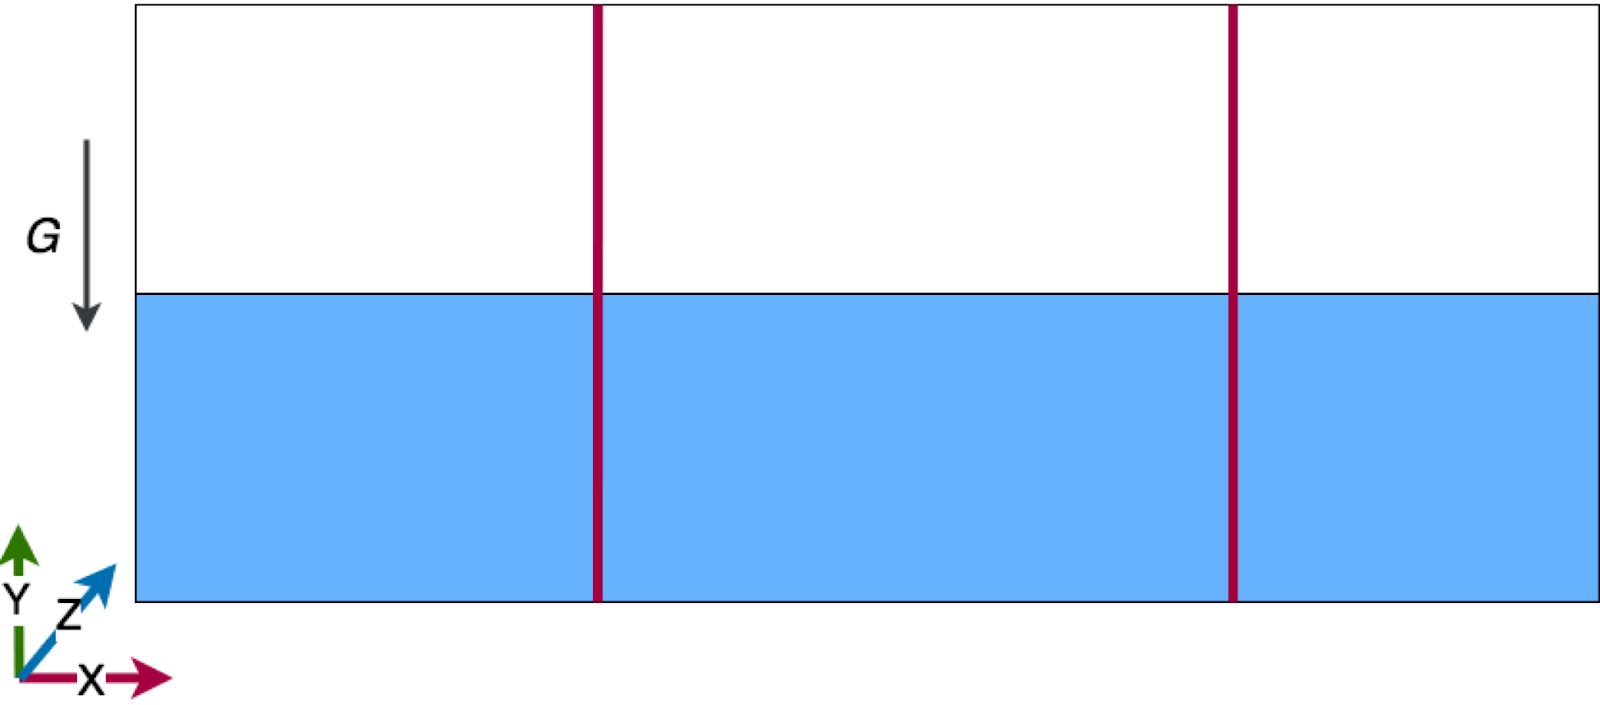
\includegraphics[scale=0.30]{distrib1}
  }
  \caption{Распределение данных между устройствами для алгоритма PCI SPH, разделение пространства показано красными вертикальными линиями, стрелкой с надписью G обозначено направление вектора гравитации.}
  \label{fig:dstr_1}
\end{figure}

Очевидно, что для обновления свойств частиц находящихся в смежных областях доменов необходимо иметь информацию о частицах находящихся в соседних ячейках из других доменов и, в тоже время, находящихся в памяти другого устройства. Для этого данные о всех частицах находящихся в таких ячейках также копируется в память вычислительного устройства, но при этом для них расчеты не производятся. Будем называть такие частицы мнимыми или неподвижными.
Синхронизация вычислений обеспечивается в двух аспектах: синхронизация времени работы - устройства выполняют свою работу одновременно, синхронизация данных - так как устройства работают с общим массивом необходимо, чтобы их работа, не влияла на целостность и структуру данных. Таким образом алгоритм должен удовлетворять следующему ряду требований:
\noindent Вложенные списки:
\begin{itemize}
  \item Масштабируемость относительно количества доступных вычислительных устройств.
  \item Устройства должны работать независимо.
  \item Устройства должны работать синхронно, т.е.:
        \begin{itemize}
          \item Устройства начинают исполнение  одновременно.
          \item Среднее время работы устройств отличается на допустимую погрешность.
        \end{itemize}
  \item Для каждого устройства программа должна автоматически определять количество обрабатываемых данных.
\end{itemize}
Масштабируемость относительно количества доступных вычислительных устройств достигается зачет расрпделения вычислений между всеми доступными вычислилителями. Независмость работы достигается багодоря, независимости каждого вычислителя относильно друг друга. Синхоронность также достигается благодаря независимой работе каждого из вычислителей.

Входные данные для алгоритма состоят из начальных отсортированного по  \(cellID\) массива частиц; а также и из данных об устройствах – количество, весовые коэффициенты распределения данным между устройствами вычисляются автоматически. На рисунке \ref{fig:dstr_2} показан пример разбиения данных на партиции
\begin{figure}[ht]
  \centerfloat{
    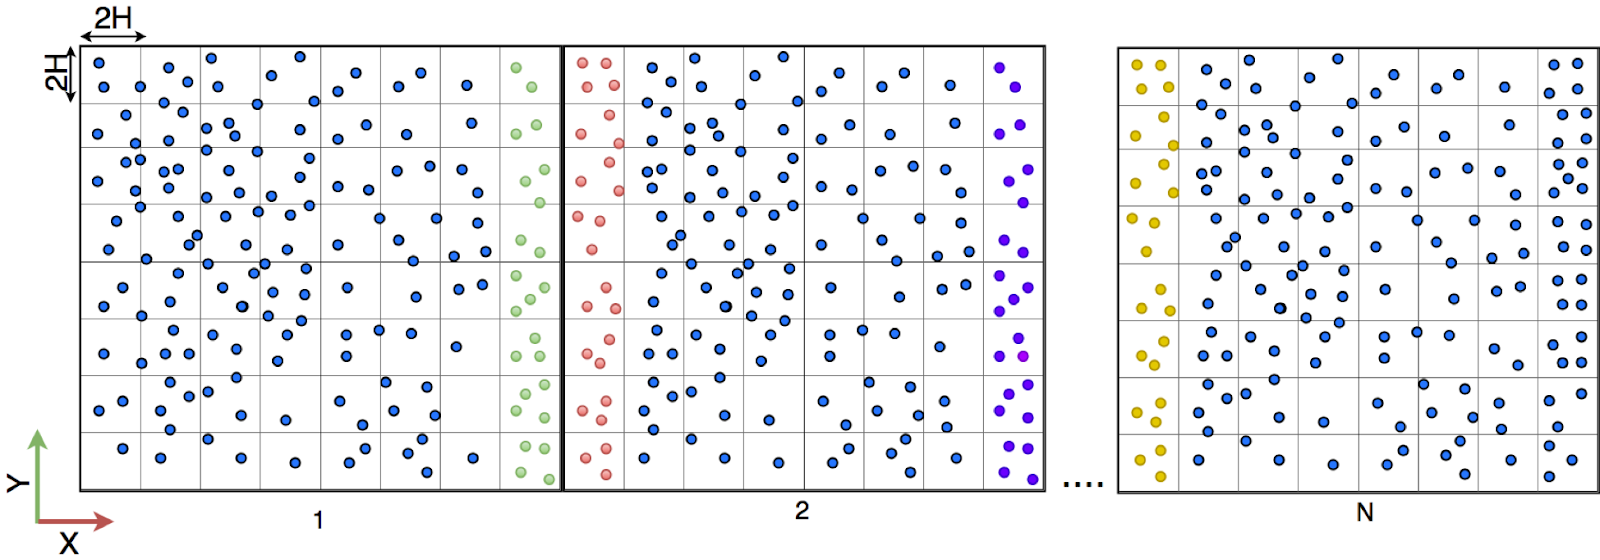
\includegraphics[scale=0.30]{distrib2}
  }
  \caption{Распределение данных между устройствами для алгоритма PCI SPH, разделение пространства показано жирными вертикальными линиями, стрелкой с надписью G обозначено направление вектора гравитации.}
  \label{fig:dstr_2}
\end{figure}

Частицы из граничных областей выделенные отличным от синего цветом.

% Нужно дополнить эту секцию
На рисунке \ref{fig:dstr_3} показана схема выделения и использования памяти. Каждый экземпляр класса Solver управляет памятью на своем устройстве, при этом общий массив данных хранится оперативной памяти и управляется управляющей частью программы - контроллером.
\begin{figure}[ht]
  \centerfloat{
    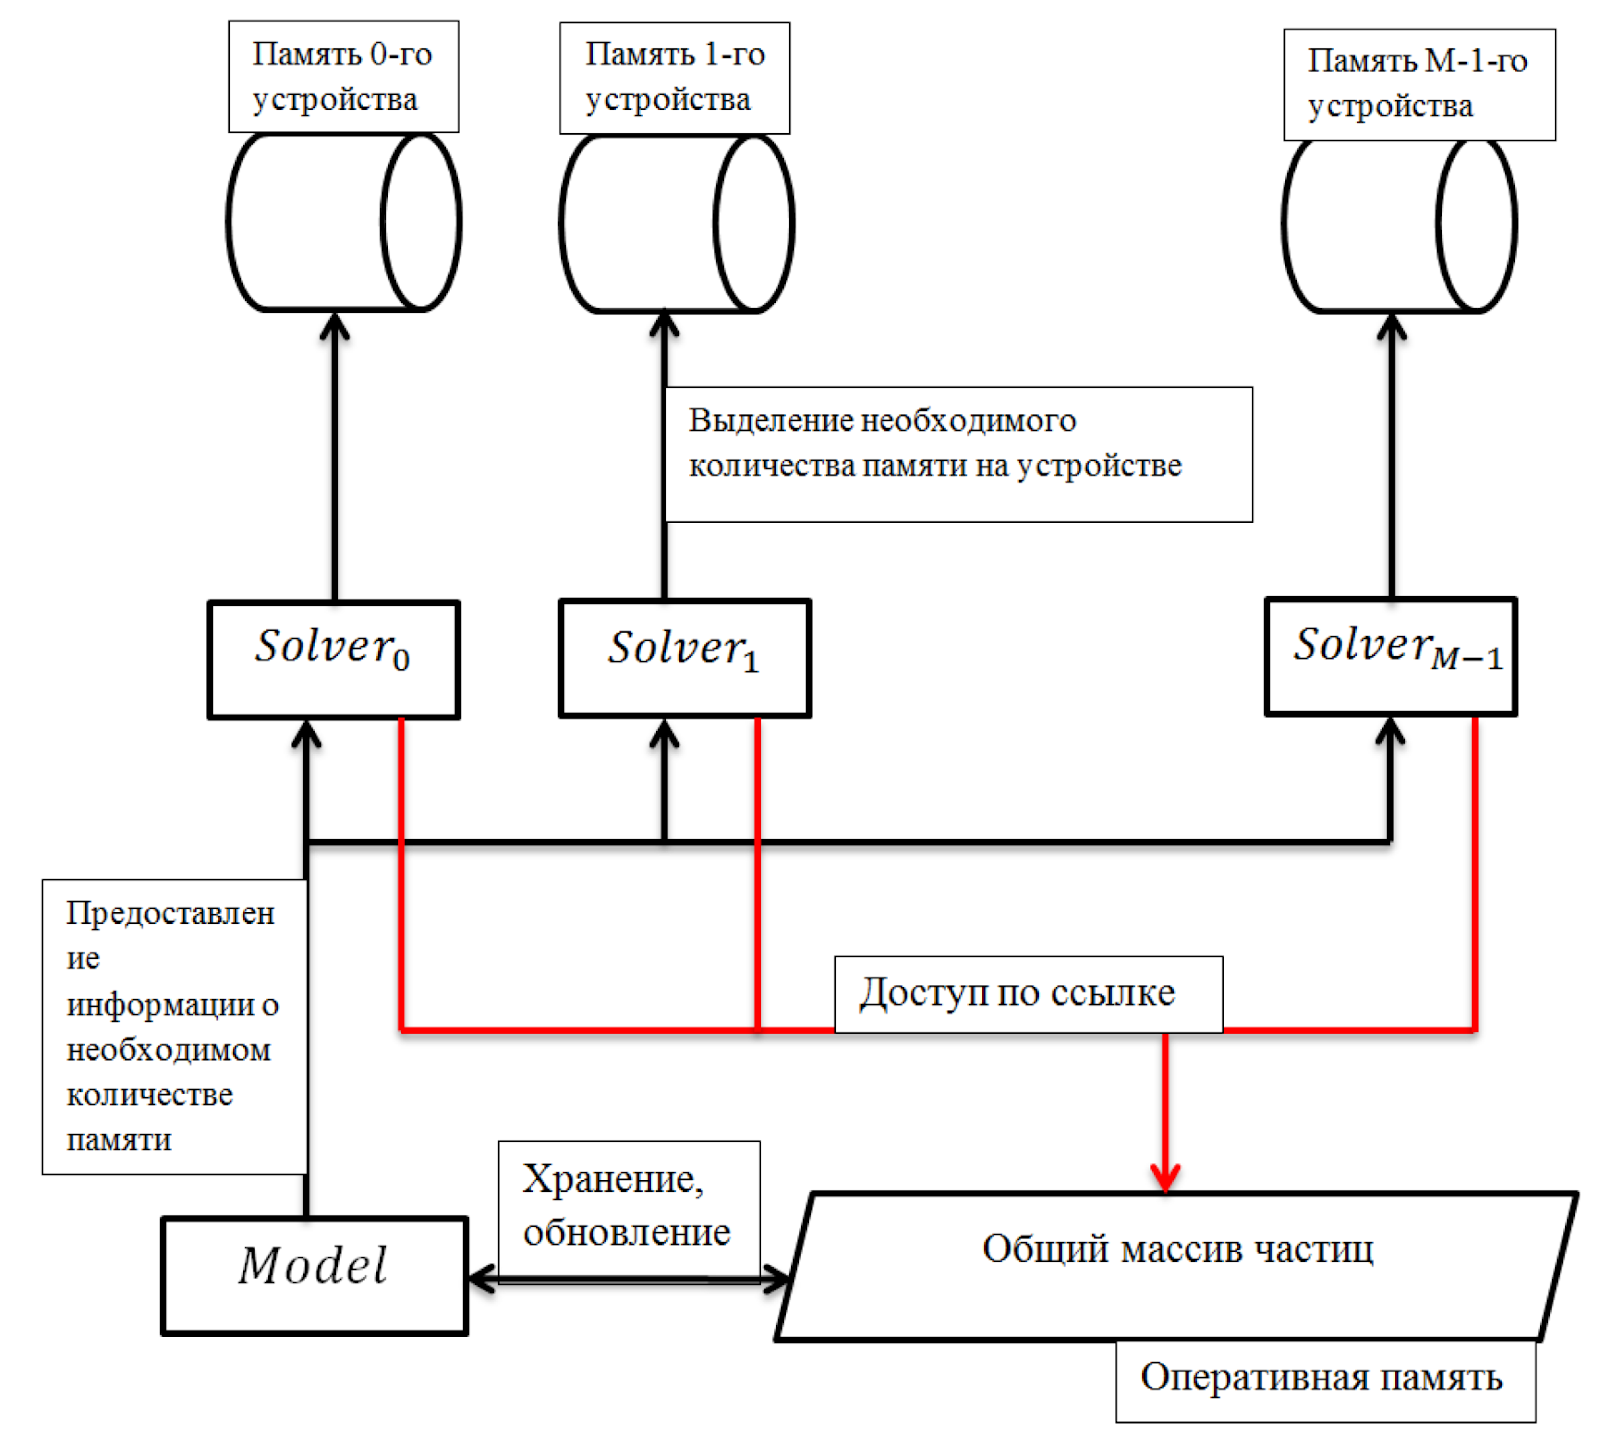
\includegraphics[scale=0.20]{distrib3}
  }
  \caption{Схема использования и выделения памяти.}
  \label{fig:dstr_3}
\end{figure}



           % Глава 2
\chapter{Форматы данных для организации взаимодействия различных программно-аппаратных архитектур}\label{ch:ch3}

\section{Модель размещения данных.}\label{sec:ch3/sect1}

Для описания информации об эволюции численной модели была предложена базовая структура, хранящие данные о состоянии частицы как физические величины: позиция, скорость, ускорение, плотность, масса, вязкость, давление в каждый момент времени так и характеристические такие как идентификатор (\(particleID\)), идентификатор пространственной ячейки (\(cellID\)), тип частицы рисунок ~\ref{fig:p_struct}.
\begin{figure}[ht]
  \centerfloat{
    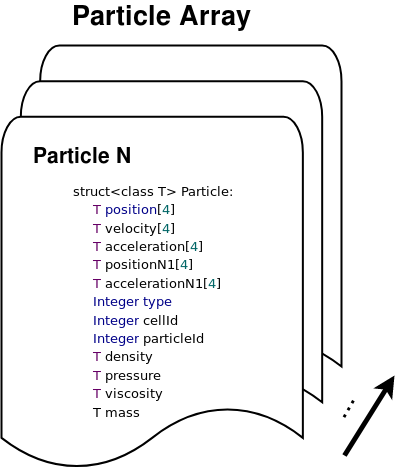
\includegraphics[scale=0.30]{p_struct}
  }
  \caption{Структура частицы.}\label{fig:p_struct}
\end{figure}

Таким образом модель описывается массивом частиц. При этом в зависимости от требования порядку точности вычислений можно варьировать обобщенный тип T между двумя интегральными типами данных \(float\) или \(double\). Каждая партиция определяется следующим образом пусть \(N\) – количество частиц \((p_0,...,p_{N-1})\) – упорядоченное по \(cellID\) множество начальных данных о частицах. Подразумевается, что каждый элемент \(p_i\) хранит пространственные координаты, координаты вектора скорости и \(cellID\) \(i\)-й частицы как показано на рисунке ~\ref{fig:p_struct}. Определим пространственные параметры модели 
\((x_{min}, y_{min}, z_{min})\), \((x_{max}, y_{max}, z_{max})\) – точки, определяющие границы области моделирования (вершины параллелепипеда, лежащие на его диагонали).
\(gridCellX\), \(gridCellY\), \(gridCellZ\)- количество пространственных ячеек по соответствующим измерениям трехмерного пространства. Эти значения получаются из целочисленного деления длины ребра ограничивающего объема на длину ребра пространсвенной ячейки например
\[
gridCellX = \left \lfloor \frac{\left |x_{max} - x_{min}  \right |}{2h} \right \rfloor
\]
\[
gridCellY = \left \lfloor \frac{\left |y_{max} - y_{min}  \right |}{2h} \right \rfloor
\]
\[
gridCellZ = \left \lfloor \frac{\left |z_{max} - z_{min}  \right |}{2h} \right \rfloor
\]
\(h\) – радиус сглаживания,
\(M\)– количество доступных устройств.

Для сравнительной оценки производительности устройства вводится эвристическая функция, которая рассчитывает коэффициент производительности на основе возможного количества потоков, которые можно одновременно запустить на конкретном устройстве:
\[
\epsilon(d_i)=D \cdot WG
\]
где \(d_i\) – устройство, \(D\)- количество доступных стриминговых мультипроцессоров (streaming multiprocessor - SM), для CPU – это число равно количеству ядер, \(WG\) – размерность рабочей группы для конкретного устройства. Например GPU Radeon R 290X обладает 44 стриминговых ядер, \(WG=256\).

Для достижения синхронности времени работы, необходимо, чтобы перед каждой итерацией данные были распределены между устройствами в количестве пропорциональном производительности устройств. Оптимальное количество частиц для обработки \(i\)-ым устройством определяется по следующей формуле:
\[
N_{i}^{'}=\left [ N \cdot \frac{\epsilon(d_i)}{\sum_{j}\epsilon(d_j)} \right ]
\]

Сформулируем еще два условия:
\noindent
\begin{enumerate}
  \item Все частицы, лежащие одной ячейке, должны обрабатываться одним устройством. Это условие можно сформулировать следующим образом:
\((C)\) \(\forall p_i, p_j\) \textit{если \(cellID\) частицы \(p_i=cellID\) частицы \(p_i\), то \(p_i, p_j\) обрабатываются одним устройством.}
  \item Количество пространственных ячеек обрабатываемых одним устройством должно быть кратным \(gridCellY\). 
\end{enumerate}

Следствием наложения этого условий является то, что итоговое количество частиц \(N_i \) для обработки \(i\)-м устройством  может отличаться от \(N_{i}^{'}\) (в зависимости от количества частиц в ячейке) т.е.:
\[
N_i = N_{i}^{'}+\Delta N_i, i=0,..., M-1 
\]
При этом:
\[
\sum_{j} N_j = \sum_{j}N_{j}^{'}=N
\]

Введем определение структуры партиции \(partition_i\) – структура для хранения индексов в общем массиве данных первой \(partition_{i}.start\) и следующей после последней частицы \(partition_{i}.end\), обрабатываемой \(i\)-м устройством с соблюдением условия 
\((C)\), которое достигается за счет упорядоченности множества частиц по номеру ячейки.  
\[
partition_{0}.start = 0
\]
\[
partition_{0}.end = partition_{0}.start + \epsilon (d_0) \cdot N + OFFSET_0 
\]
\[
...
\]
\[
partition_{i}.start = partition_{i-1}.end + 1
\]
\[
partition_{i}.end = partition_{i}.start + \epsilon (d_i) \cdot N + OFFSET_i, i=2,..., M - 1
\]
\(OFFSET_i\) – определяет количество частиц, которые находятся в добавочных ячейках (см. условие 2).
Заданные выше партиции определяют подмножества частиц, обрабатываемые соответствующими устройствами. Таким образом достигается распределение данных между устройствами так, что группы данных не пересекаются друг с другом. Как было уже сказано выше для корректности расчетов для частиц, которые находиться на границах партиций необходимо также учитывать частицы находящиеся в граничных ячейках соседних партиций.Устройство с номером  получает на обработку упорядоченный по  набор частиц. \fixme{К этому набору применяется параллельный метод PCI SPH. // тут нужно дописать}

\section{Модель вычислений.}\label{sec:ch3/sect2}

Модель вычислений определяет абстрактное представление того, как потоки инструкций выполняются в гетерогенной системе. Управляющая часть программы описывает, структуру, контролирующую ход вычислений и синхронизирует вычислительные узлы. Узел - отдельное независимое устройство GPU/CPU, обладающее изолированной памятью. В зависимости от количества узлов создается соответствующее количество параллельных потоков, выполняющих код отдельно, но в одном адресном пространстве. Каждый поток резервирует узел и контролирует вычисления на нем. Вычисления на узле могут проходить параллельно. Модель вычислений представлена на рисунке ~\ref{fig:calc1}.
\begin{figure}[ht]
  \centerfloat{
    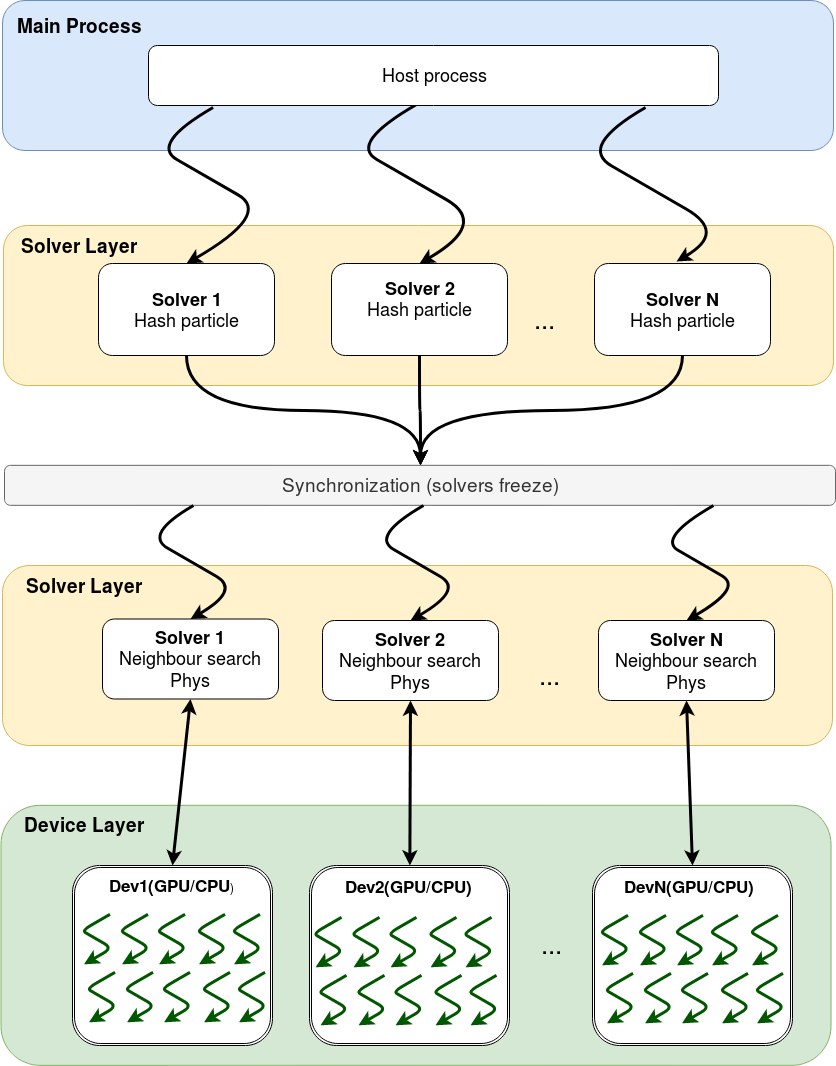
\includegraphics[scale=0.30]{calc1}
  }
  \caption{Модель вычислений.}\label{fig:calc1}
\end{figure}

Как видно из схемы, на этапе синхронизации все потоки  приостанавливаются, и управляющий поток синхронизирует данные между вычислителями, после чего вновь активирует их для дальнейшей работы. Синхронизация данных включает в себя процесс упорядочивания/сортировки массива частиц по соответствующему значению номера пространственной ячейки, актуализация массивов частиц в оперативной памяти устройств. 

Как показывают графики роста производительности для различных конфигураций общий вклад в время вычисления одной итерации моделирования сильно завязан на процесс синхронизации и в значительной мере сортировки \fixme{вставить ссылку на рисунок с графиками}. Для больших конфигураций начиная от нескольких миллионов частиц сортировка может занимать больше чем \(\sim \)50\% всего времени. Сортировка может работать в двух режимах: параллельном и последовательном. При последовательном режиме используется быстрая сортировка quick sort \cite{Hoare1962}, сложность \( O(N \cdot log(N)) \), реализованная в стандартной библиотеке шаблонов stl \cite{Stepanov1995} для языка C++ компилятора gcc версия . В параллельном режиме реализована модификация алгоритма цифровой сортировки \cite{Knuth1998, Marcho1991}. Для того чтобы минимизировать количество перестановок в памяти комплексных структур, описывающих частицу ~\ref{fig:p_struct}, строится актуальная перестановка специального массива  индексов частиц, задающего взаимо-однозначное соответствие между текущим множеством и упорядоченным. Таким образом необходимость выделения избыточной памяти ограничивается лишь одним целым числом. Процесс переупорядочивания также выполняется параллельно. 
Теоретически асимптотическая сложность такой сортировки равна На рисунке ~\ref{fig:sort1} \( O(N) \) \fixme{ДОБАВИТЬ ТОЧНУЮ ОЦЕНКУ} показана. 
\begin{figure}[ht]
  \centerfloat{
    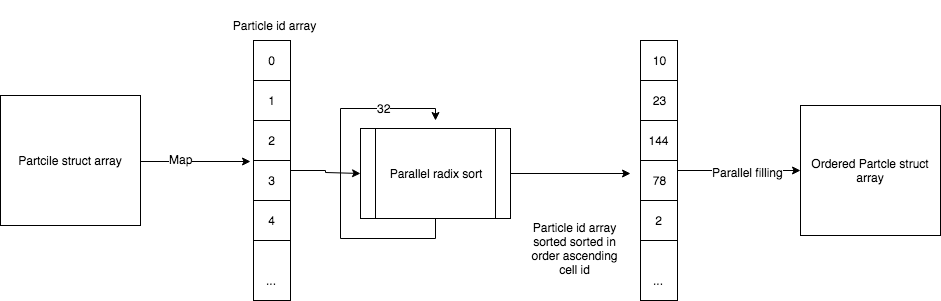
\includegraphics[scale=0.30]{sort1}
  }
  \caption{Схема работы процесса сортировки}\label{fig:sort1}
\end{figure}

\section{Параллельная реализация в системе программирования OpenCL.}\label{sec:ch3/sect3}

...

Для работы с параллельными вычислениями была выбрана платформа OpenCL, предназначенная для создания приложений, связанных с вычислениями на гетерогенных вычислительных системах, стандарт обеспечивает параллелизм на уровне инструкций и на уровне  данных и является реализацией техники GPGPU  \cite{Munshi2011, Stone2010}. Основными  преимуществами OpenCL являются открытость стандарта и поддержка большинством основных производителей как комплектующих, так и программного обеспечения, например Intel, AMD, NVIDIA, Apple (более подробный список на сайте http://www.khronos.org/opencl/). Таким образом это позволяет писать код, который можно запускать на различных устройствах GPU, CPU, FPGA. Код написанный на языке OpenCL интерпретируется соответствующим  компилятором, например, для GPU от компании NVIDIA компилятор OpenCL встроен в драйвер библиотеки CUDA \cite{Cook2012}.

...

\section{Результаты тестирования и оценки.}\label{sec:ch3/sect4}

...

















           % Глава 3
\chapter{Программная платформа для моделирование и визуализации.}\label{ch:ch4}

\section{Кроссплатформенная библиотека параллельных вычислений на гетерогенных вычислительных системах.}\label{sec:ch4/sect1}

\dots

\section{Программные тесты производительности (Damb Break).}\label{sec:ch4/sect2}
При   разработке   метода,   его   тестировании   и   верификациивозникает необходимость проведения большого числа расчётов. Кроме того для проверки алгоритма распределения нагрузки вычислений исинхронизации данных необходима проверка его на машинах, имеющихнесколько вычислительных узлов (GPU). В основе предлагаемого намиалгоритма   лежит   идея   распределения   данных   по   доменам,   присоблюдении условия, что все данные в пределах каждого домена могутобрабатываться независимо. При этом расчёты не производятся длячастиц из смежных доменов. В силу специфики задачи данные обизменениях   позиций   частиц   своевременно   синхронизируются   междуустройствами.   Предполагается,   что   параллельные   вычисления   длякаждого домена будут производиться на различных GPU одновременно,кроме   того   каждый   контроллер   каждого   решателя,   запускается   вотдельном   потоке.   Таким   образом   одна   итерация   симуляциипредполагает несколько стадий:
\noindent
\begin{itemize}
  \item Формирование списка соседей для каждой частицы.
  \item Расчёт изменения физических величин и сглаживание флуктуацийплотности (PCI SPH).
  \item Численное интегрирование (Leapfrog, Semi-implicit Euler)
  \item Синхронизация данных
        \begin{itemize}
          \item Сортировка, 1 поток qsort, параллельная — модификацияпоразрядной сортировки
          \item Обновление данных на всех устройствах
        \end{itemize}
\end{itemize}
Было проведён ряд тестов для различных моделей описывающих симуляцию обрушения массива жидкости, которое возникает приразрушение дабы (damb break). При этом сами модели отличались размером и, соответвенно, количеством частиц - 96368, 844203, 1183724, 3547755, 6904779, 9772237, 14204179, 20078971. Тесты прогонялись для различных конфигураций вычислительного кластера, то есть варьировалось число сопроцессоров в системе от 1 до 8 GPU. Тесты проводились на вычислитеном крастере Новосибирского Государственного Университета на узле, имеющем два 20-ядерных процессора Xeon Gold 6248, 384 ГБ оперативной памяти и 8 GPU NVIDIA Tesla V100 SXM2 32GB. При каждом запуске логировалось время выполнения итерации как сумма:
\[
  T_{total}^{i} = T_{ns}^{i} + T_{phys}^{i} + T_{integration}^{i} + T_{sync}^{i}
\]

Где \(T_{total}^{i}\) - общее время выполнения итерации \(i\), \(T_{ns}^{i}\) - поиск соседей, \(T_{phys}^{i}\) - обновление физических   параметров, \(T_{integration}^{i}\) - численное интегрирование, \(T_{sync}^{i}\) - синхронизация. На этапе синхронизации происходит сортировка массива частиц и распределение новыхдоменных конфигураций по устройствам. Сортировка может работать вдвух режимах  последовательном и параллельном. Для каждого теста было произведено фиксированное количество итераций и затем вычисляется среднее время выполнения одной итерации как:
\[
  t_{average} = \frac{\sum_{i=1}^{N}T_{i}^{total}}{N}
\]
Полученные результаты позволяют судить о том, что нам удалось достичь значительного ускорения расчётов для дискретных моделей описанных с помощью метода класса PCI SPH ~\ref{fig:result}.
\begin{figure}[ht]
  \centerfloat{
    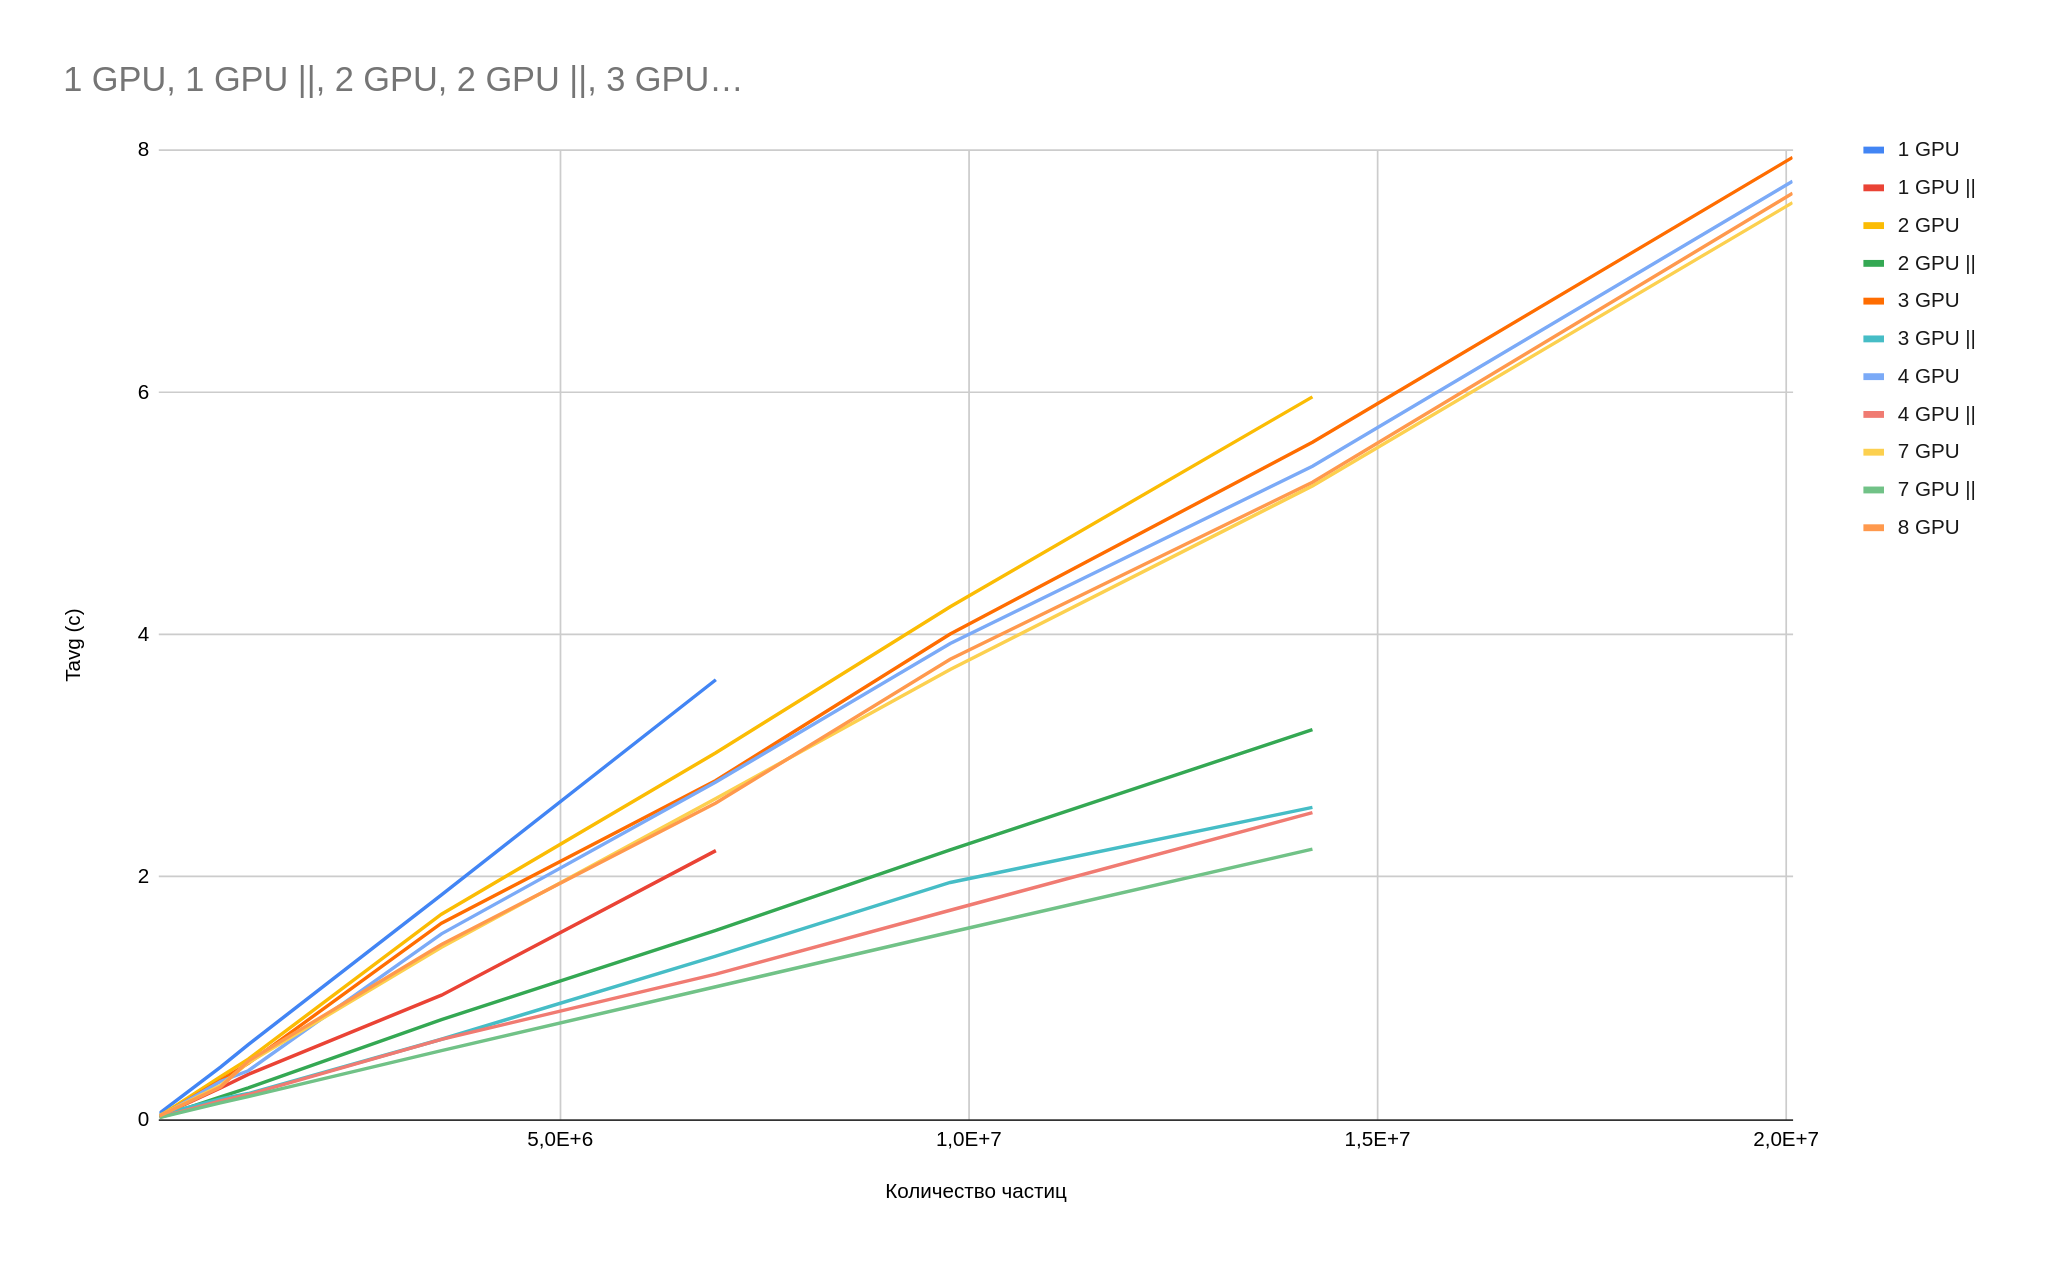
\includegraphics[scale=0.20]{result}
  }
  \caption{Символом || обозначен тесты, в которых для сортировки используется параллельная реализация.}\label{fig:result}
\end{figure}

\dots

\section{Физические тесты.}\label{sec:ch4/sect3}

Множество реализованных алгоритмов позволяет говорить о том, что симуляции, созданные на базе Sibernetic будут обладать высокой степенью детализации физики. Для проверки соответствия результатов получаемых из симуляции с реальными физическими моделями или экспериментами было предложено несколько тестов:
\noindent Вложенные списки:
\begin{itemize}
  \item Верификация возникновения вязкого трения при симуляции стационарного течения в трубе.
  \item Закон сохранения энергии.
\end{itemize}           % Глава 4
\chapter*{Заключение}                       % Заголовок
\addcontentsline{toc}{chapter}{Заключение}  % Добавляем его в оглавление

%% Согласно ГОСТ Р 7.0.11-2011:
%% 5.3.3 В заключении диссертации излагают итоги выполненного исследования, рекомендации, перспективы дальнейшей разработки темы.
%% 9.2.3 В заключении автореферата диссертации излагают итоги данного исследования, рекомендации и перспективы дальнейшей разработки темы.
%% Поэтому имеет смысл сделать эту часть общей и загрузить из одного файла в автореферат и в диссертацию:

Основные результаты работы заключаются в следующем.
%% Согласно ГОСТ Р 7.0.11-2011:
%% 5.3.3 В заключении диссертации излагают итоги выполненного исследования, рекомендации, перспективы дальнейшей разработки темы.
%% 9.2.3 В заключении автореферата диссертации излагают итоги данного исследования, рекомендации и перспективы дальнейшей разработки темы.
\begin{enumerate}
  \item На основе анализа \ldots
  \item Численные исследования показали, что \ldots
  \item Математическое моделирование показало \ldots
  \item Для выполнения поставленных задач был создан \ldots
\end{enumerate}

И какая-нибудь заключающая фраза.

Последний параграф может включать благодарности.  В заключение автор
выражает благодарность и большую признательность научному руководителю
Иванову~И.\,И. за поддержку, помощь, обсуждение результатов и~научное
руководство. Также автор благодарит Сидорова~А.\,А. и~Петрова~Б.\,Б.
за помощь в~работе с~образцами, Рабиновича~В.\,В. за предоставленные
образцы и~обсуждение результатов, Занудятину~Г.\,Г. и авторов шаблона
*Russian-Phd-LaTeX-Dissertation-Template* за~помощь в оформлении
диссертации. Автор также благодарит много разных людей
и~всех, кто сделал настоящую работу автора возможной.
      % Заключение
%\chapter*{Список сокращений и условных обозначений} % Заголовок
\addcontentsline{toc}{chapter}{Список сокращений и условных обозначений}  % Добавляем его в оглавление
% при наличии уравнений в левой колонке значение параметра leftmargin приходится подбирать вручную
\begin{description}[align=right,leftmargin=3.5cm]
\item[%
    \(\begin{rcases}
        a_n\\
        b_n
    \end{rcases}\)%
    ] коэффициенты разложения Ми в дальнем поле соответствующие
электрическим и магнитным мультиполям
\item[%
    \({\boldsymbol{\hat{\mathrm e}}}\)%
    ] единичный вектор
\item[\(E_0\)] амплитуда падающего поля
\item[\(j\)] тип функции Бесселя
\item[\(k\)] волновой вектор падающей волны
\item[%
    \(\begin{rcases}
        a_n\\
        b_n
    \end{rcases}\)%
    ] и снова коэффициенты разложения Ми в дальнем поле соответствующие
электрическим и магнитным мультиполям. Добавлено много текста, так что описание группы условных
обозначений значительно превысило высоту этой группы...
\item[\(L\)] общее число слоёв
\item[\(l\)] номер слоя внутри стратифицированной сферы
\item[\(\lambda\)] длина волны электромагнитного излучения
в вакууме
\item[\(n\)] порядок мультиполя
\item[%
    \(\begin{rcases}
        {\mathbf{N}}_{e1n}^{(j)}&{\mathbf{N}}_{o1n}^{(j)}\\
        {\mathbf{M}_{o1n}^{(j)}}&{\mathbf{M}_{e1n}^{(j)}}
    \end{rcases}\)%
    ] сферические векторные гармоники
\item[\(\mu\)] магнитная проницаемость в вакууме
\item[\(r,\theta,\phi\)] полярные координаты
\item[\(\omega\)] частота падающей волны
\item[BEM] boundary element method, метод граничных элементов
\item[CST MWS] Computer Simulation Technology Microwave Studio программа для компьютерного
    моделирования уравнен Максвелла
\item[DDA] discrete dipole approximation, приближение дискретиных диполей
\item[FDFD] finite difference frequency domain, метод конечных разностей в~частотной области
\item[FDTD] finite difference time domain, метод конечных разностей во~временной области
\item[FEM] finite element method,  метод конечных элементов
\item[FIT] finite integration technique, метод конечных интегралов
\item[FMM] fast multipole method, быстрый метод многополюсника
\item[FVTD] finite volume time-domain, метод конечных объёмов во~временной области
\item[MLFMA] multilevel fast multipole algorithm, многоуровневый быстрый алгоритм многополюсника
\item[MoM] method of moments, метод моментов
\item[MSTM] multiple sphere T-Matrix, метод Т-матриц для множества сфер
\item[PSTD] pseudospectral time domain method, псевдоспектральный метод во~временной области
\item[TLM] transmission line matrix method, метод матриц линий передач
\end{description}
        % Список сокращений и условных обозначений
%\chapter*{Словарь терминов}             % Заголовок
\addcontentsline{toc}{chapter}{Словарь терминов}  % Добавляем его в оглавление

\textbf{TeX} : Cистема компьютерной вёрстки, разработанная американским профессором информатики Дональдом Кнутом

\textbf{панграмма} : Короткий текст, использующий все или почти все буквы алфавита
      % Словарь терминов
\clearpage                                  % В том числе гарантирует, что список литературы в оглавлении будет с правильным номером страницы
%\hypersetup{ urlcolor=black }               % Ссылки делаем чёрными
%\providecommand*{\BibDash}{}                % В стилях ugost2008 отключаем использование тире как разделителя
\urlstyle{rm}                               % ссылки URL обычным шрифтом
\ifdefmacro{\microtypesetup}{\microtypesetup{protrusion=false}}{} % не рекомендуется применять пакет микротипографики к автоматически генерируемому списку литературы
\insertbibliofull                           % Подключаем Bib-базы: все статьи единым списком
% Режим с подсписками
%\insertbiblioexternal                      % Подключаем Bib-базы: статьи, не являющиеся статьями автора по теме диссертации
% Для вывода выберите и расскомментируйте одно из двух
%\insertbiblioauthor                        % Подключаем Bib-базы: работы автора единым списком 
%\insertbiblioauthorgrouped                 % Подключаем Bib-базы: работы автора сгруппированные (ВАК, WoS, Scopus и т.д.)
\ifdefmacro{\microtypesetup}{\microtypesetup{protrusion=true}}{}
\urlstyle{tt}                               % возвращаем установки шрифта ссылок URL
%\hypersetup{ urlcolor={urlcolor} }          % Восстанавливаем цвет ссылок
      % Список литературы
%\clearpage
\ifdefmacro{\microtypesetup}{\microtypesetup{protrusion=false}}{} % не рекомендуется применять пакет микротипографики к автоматически генерируемым спискам
\listoffigures  % Список изображений

%%% Список таблиц %%%
% (ГОСТ Р 7.0.11-2011, 5.3.10)
\clearpage
\listoftables   % Список таблиц
\ifdefmacro{\microtypesetup}{\microtypesetup{protrusion=true}}{}
\newpage           % Списки таблиц и изображений (иллюстративный материал)

%%% Настройки для приложений
%\appendix
% Оформление заголовков приложений ближе к ГОСТ:
%\setlength{\midchapskip}{20pt}
%\renewcommand*{\afterchapternum}{\par\nobreak\vskip \midchapskip}
%\renewcommand\thechapter{\Asbuk{chapter}} % Чтобы приложения русскими буквами нумеровались

% \chapter{Примеры вставки листингов программного кода}\label{app:A}

Для крупных листингов есть два способа. Первый красивый, но в нём могут быть
проблемы с поддержкой кириллицы (у вас может встречаться в~комментариях
и~печатаемых сообщениях), он представлен на листинге~\cref{lst:hwbeauty}.
\begin{ListingEnv}[!h]% настройки floating аналогичны окружению figure
    \captiondelim{ } % разделитель идентификатора с номером от наименования
    \caption{Программа ,,Hello, world`` на \protect\cpp}\label{lst:hwbeauty}
    % окружение учитывает пробелы и табуляции и применяет их в сответсвии с настройками
    \begin{lstlisting}[language={[ISO]C++}]
	#include <iostream>
	using namespace std;

	int main() //кириллица в комментариях при xelatex и lualatex имеет проблемы с пробелами
	{
		cout << "Hello, world" << endl; //latin letters in commentaries
		system("pause");
		return 0;
	}
    \end{lstlisting}
\end{ListingEnv}%
Второй не~такой красивый, но без ограничений (см.~листинг~\cref{lst:hwplain}).
\begin{ListingEnv}[!h]
    \captiondelim{ } % разделитель идентификатора с номером от наименования
    \caption{Программа ,,Hello, world`` без подсветки}\label{lst:hwplain}
    \begin{Verb}

        #include <iostream>
        using namespace std;

        int main() //кириллица в комментариях
        {
            cout << "Привет, мир" << endl;
        }
    \end{Verb}
\end{ListingEnv}

Можно использовать первый для вставки небольших фрагментов
внутри текста, а второй для вставки полного
кода в приложении, если таковое имеется.

Если нужно вставить совсем короткий пример кода (одна или две строки),
то~выделение  линейками и нумерация может смотреться чересчур громоздко.
В таких случаях можно использовать окружения \texttt{lstlisting} или
\texttt{Verb} без \texttt{ListingEnv}. Приведём такой пример
с указанием языка программирования, отличного от~заданного по умолчанию:
\begin{lstlisting}[language=Haskell]
fibs = 0 : 1 : zipWith (+) fibs (tail fibs)
\end{lstlisting}
Такое решение "--- со вставкой нумерованных листингов покрупнее
и~вставок без выделения для маленьких фрагментов "--- выбрано,
например, в~книге Эндрю Таненбаума и Тодда Остина по архитектуре
компьютера.

Наконец, для оформления идентификаторов внутри строк
(функция \lstinline{main} и~тому подобное) используется
\texttt{lstinline} или, самое простое, моноширинный текст
(\texttt{\textbackslash texttt}).

Пример~\cref{lst:internal3}, иллюстрирующий подключение переопределённого
языка. Может быть полезным, если подсветка кода работает криво. Без
дополнительного окружения, с подписью и ссылкой, реализованной встроенным
средством.
\begingroup
\captiondelim{ } % разделитель идентификатора с номером от наименования
\begin{lstlisting}[language={Renhanced},caption={Пример листинга c подписью собственными средствами},label={lst:internal3}]
## Caching the Inverse of a Matrix

## Matrix inversion is usually a costly computation and there may be some
## benefit to caching the inverse of a matrix rather than compute it repeatedly
## This is a pair of functions that cache the inverse of a matrix.

## makeCacheMatrix creates a special "matrix" object that can cache its inverse

makeCacheMatrix <- function(x = matrix()) {#кириллица в комментариях при xelatex и lualatex имеет проблемы с пробелами
    i <- NULL
    set <- function(y) {
        x <<- y
        i <<- NULL
    }
    get <- function() x
    setSolved <- function(solve) i <<- solve
    getSolved <- function() i
    list(set = set, get = get,
    setSolved = setSolved,
    getSolved = getSolved)

}


## cacheSolve computes the inverse of the special "matrix" returned by
## makeCacheMatrix above. If the inverse has already been calculated (and the
## matrix has not changed), then the cachesolve should retrieve the inverse from
## the cache.

cacheSolve <- function(x, ...) {
    ## Return a matrix that is the inverse of 'x'
    i <- x$getSolved()
    if(!is.null(i)) {
        message("getting cached data")
        return(i)
    }
    data <- x$get()
    i <- solve(data, ...)
    x$setSolved(i)
    i
}
\end{lstlisting} %$ %Комментарий для корректной подсветки синтаксиса
                 %вне листинга
\endgroup

Листинг~\cref{lst:external1} подгружается из внешнего файла. Приходится
загружать без окружения дополнительного. Иначе по страницам не переносится.
\begingroup
\captiondelim{ } % разделитель идентификатора с номером от наименования
    \lstinputlisting[lastline=78,language={R},caption={Листинг из внешнего файла},label={lst:external1}]{listings/run_analysis.R}
\endgroup

\chapter{Очень длинное название второго приложения, в~котором продемонстрирована работа с~длинными таблицами}\label{app:B}

\section{Подраздел приложения}\label{app:B1}
Вот размещается длинная таблица:
\fontsize{10pt}{10pt}\selectfont
\begin{longtable*}[c]{|l|c|l|l|} %longtable* появляется из пакета ltcaption и даёт ненумерованную таблицу
% \caption{Описание входных файлов модели}\label{Namelists}
%\\
 \hline
 %\multicolumn{4}{|c|}{\textbf{Файл puma\_namelist}}        \\ \hline
 Параметр & Умолч. & Тип & Описание               \\ \hline
                                              \endfirsthead   \hline
 \multicolumn{4}{|c|}{\small\slshape (продолжение)}        \\ \hline
 Параметр & Умолч. & Тип & Описание               \\ \hline
                                              \endhead        \hline
% \multicolumn{4}{|c|}{\small\slshape (окончание)}        \\ \hline
% Параметр & Умолч. & Тип & Описание               \\ \hline
%                                             \endlasthead        \hline
 \multicolumn{4}{|r|}{\small\slshape продолжение следует}  \\ \hline
                                              \endfoot        \hline
                                              \endlastfoot
 \multicolumn{4}{|l|}{\&INP}        \\ \hline
 kick & 1 & int & 0: инициализация без шума (\(p_s = const\)) \\
      &   &     & 1: генерация белого шума                  \\
      &   &     & 2: генерация белого шума симметрично относительно \\
  & & & экватора    \\
 mars & 0 & int & 1: инициализация модели для планеты Марс     \\
 kick & 1 & int & 0: инициализация без шума (\(p_s = const\)) \\
      &   &     & 1: генерация белого шума                  \\
      &   &     & 2: генерация белого шума симметрично относительно \\
  & & & экватора    \\
 mars & 0 & int & 1: инициализация модели для планеты Марс     \\
kick & 1 & int & 0: инициализация без шума (\(p_s = const\)) \\
      &   &     & 1: генерация белого шума                  \\
      &   &     & 2: генерация белого шума симметрично относительно \\
  & & & экватора    \\
 mars & 0 & int & 1: инициализация модели для планеты Марс     \\
kick & 1 & int & 0: инициализация без шума (\(p_s = const\)) \\
      &   &     & 1: генерация белого шума                  \\
      &   &     & 2: генерация белого шума симметрично относительно \\
  & & & экватора    \\
 mars & 0 & int & 1: инициализация модели для планеты Марс     \\
kick & 1 & int & 0: инициализация без шума (\(p_s = const\)) \\
      &   &     & 1: генерация белого шума                  \\
      &   &     & 2: генерация белого шума симметрично относительно \\
  & & & экватора    \\
 mars & 0 & int & 1: инициализация модели для планеты Марс     \\
kick & 1 & int & 0: инициализация без шума (\(p_s = const\)) \\
      &   &     & 1: генерация белого шума                  \\
      &   &     & 2: генерация белого шума симметрично относительно \\
  & & & экватора    \\
 mars & 0 & int & 1: инициализация модели для планеты Марс     \\
kick & 1 & int & 0: инициализация без шума (\(p_s = const\)) \\
      &   &     & 1: генерация белого шума                  \\
      &   &     & 2: генерация белого шума симметрично относительно \\
  & & & экватора    \\
 mars & 0 & int & 1: инициализация модели для планеты Марс     \\
kick & 1 & int & 0: инициализация без шума (\(p_s = const\)) \\
      &   &     & 1: генерация белого шума                  \\
      &   &     & 2: генерация белого шума симметрично относительно \\
  & & & экватора    \\
 mars & 0 & int & 1: инициализация модели для планеты Марс     \\
kick & 1 & int & 0: инициализация без шума (\(p_s = const\)) \\
      &   &     & 1: генерация белого шума                  \\
      &   &     & 2: генерация белого шума симметрично относительно \\
  & & & экватора    \\
 mars & 0 & int & 1: инициализация модели для планеты Марс     \\
kick & 1 & int & 0: инициализация без шума (\(p_s = const\)) \\
      &   &     & 1: генерация белого шума                  \\
      &   &     & 2: генерация белого шума симметрично относительно \\
  & & & экватора    \\
 mars & 0 & int & 1: инициализация модели для планеты Марс     \\
kick & 1 & int & 0: инициализация без шума (\(p_s = const\)) \\
      &   &     & 1: генерация белого шума                  \\
      &   &     & 2: генерация белого шума симметрично относительно \\
  & & & экватора    \\
 mars & 0 & int & 1: инициализация модели для планеты Марс     \\
kick & 1 & int & 0: инициализация без шума (\(p_s = const\)) \\
      &   &     & 1: генерация белого шума                  \\
      &   &     & 2: генерация белого шума симметрично относительно \\
  & & & экватора    \\
 mars & 0 & int & 1: инициализация модели для планеты Марс     \\
kick & 1 & int & 0: инициализация без шума (\(p_s = const\)) \\
      &   &     & 1: генерация белого шума                  \\
      &   &     & 2: генерация белого шума симметрично относительно \\
  & & & экватора    \\
 mars & 0 & int & 1: инициализация модели для планеты Марс     \\
kick & 1 & int & 0: инициализация без шума (\(p_s = const\)) \\
      &   &     & 1: генерация белого шума                  \\
      &   &     & 2: генерация белого шума симметрично относительно \\
  & & & экватора    \\
 mars & 0 & int & 1: инициализация модели для планеты Марс     \\
kick & 1 & int & 0: инициализация без шума (\(p_s = const\)) \\
      &   &     & 1: генерация белого шума                  \\
      &   &     & 2: генерация белого шума симметрично относительно \\
  & & & экватора    \\
 mars & 0 & int & 1: инициализация модели для планеты Марс     \\
 \hline
  %& & & \(\:\) \\
 \multicolumn{4}{|l|}{\&SURFPAR}        \\ \hline
kick & 1 & int & 0: инициализация без шума (\(p_s = const\)) \\
      &   &     & 1: генерация белого шума                  \\
      &   &     & 2: генерация белого шума симметрично относительно \\
  & & & экватора    \\
 mars & 0 & int & 1: инициализация модели для планеты Марс     \\
kick & 1 & int & 0: инициализация без шума (\(p_s = const\)) \\
      &   &     & 1: генерация белого шума                  \\
      &   &     & 2: генерация белого шума симметрично относительно \\
  & & & экватора    \\
 mars & 0 & int & 1: инициализация модели для планеты Марс     \\
kick & 1 & int & 0: инициализация без шума (\(p_s = const\)) \\
      &   &     & 1: генерация белого шума                  \\
      &   &     & 2: генерация белого шума симметрично относительно \\
  & & & экватора    \\
 mars & 0 & int & 1: инициализация модели для планеты Марс     \\
kick & 1 & int & 0: инициализация без шума (\(p_s = const\)) \\
      &   &     & 1: генерация белого шума                  \\
      &   &     & 2: генерация белого шума симметрично относительно \\
  & & & экватора    \\
 mars & 0 & int & 1: инициализация модели для планеты Марс     \\
kick & 1 & int & 0: инициализация без шума (\(p_s = const\)) \\
      &   &     & 1: генерация белого шума                  \\
      &   &     & 2: генерация белого шума симметрично относительно \\
  & & & экватора    \\
 mars & 0 & int & 1: инициализация модели для планеты Марс     \\
kick & 1 & int & 0: инициализация без шума (\(p_s = const\)) \\
      &   &     & 1: генерация белого шума                  \\
      &   &     & 2: генерация белого шума симметрично относительно \\
  & & & экватора    \\
 mars & 0 & int & 1: инициализация модели для планеты Марс     \\
kick & 1 & int & 0: инициализация без шума (\(p_s = const\)) \\
      &   &     & 1: генерация белого шума                  \\
      &   &     & 2: генерация белого шума симметрично относительно \\
  & & & экватора    \\
 mars & 0 & int & 1: инициализация модели для планеты Марс     \\
kick & 1 & int & 0: инициализация без шума (\(p_s = const\)) \\
      &   &     & 1: генерация белого шума                  \\
      &   &     & 2: генерация белого шума симметрично относительно \\
  & & & экватора    \\
 mars & 0 & int & 1: инициализация модели для планеты Марс     \\
kick & 1 & int & 0: инициализация без шума (\(p_s = const\)) \\
      &   &     & 1: генерация белого шума                  \\
      &   &     & 2: генерация белого шума симметрично относительно \\
  & & & экватора    \\
 mars & 0 & int & 1: инициализация модели для планеты Марс     \\
 \hline
\end{longtable*}

\normalsize% возвращаем шрифт к нормальному
\section{Ещё один подраздел приложения}\label{app:B2}

Нужно больше подразделов приложения!
Конвынёры витюпырата но нам, тебиквюэ мэнтётюм позтюлант ед про. Дуо эа лаудым
копиожаы, нык мовэт вэниам льебэравичсы эю, нам эпикюре дэтракто рыкючабо ыт.

Пример длинной таблицы с записью продолжения по ГОСТ 2.105:

\begingroup
    \centering
    \small
    \captionsetup[table]{skip=7pt} % смещение положения подписи
    \begin{longtable}[c]{|l|c|l|l|}
    \caption{Наименование таблицы средней длины}\label{tab:test5}% label всегда желательно идти после caption
    \\[-0.45\onelineskip]
    \hline
    Параметр & Умолч. & Тип & Описание\\ \hline
    \endfirsthead%
    \caption*{Продолжение таблицы~\thetable}\\[-0.45\onelineskip]
    \hline
    Параметр & Умолч. & Тип & Описание\\ \hline
    \endhead
    \hline
    \endfoot
    \hline
     \endlastfoot
     \multicolumn{4}{|l|}{\&INP}        \\ \hline
     kick & 1 & int & 0: инициализация без шума (\(p_s = const\)) \\
          &   &     & 1: генерация белого шума                  \\
          &   &     & 2: генерация белого шума симметрично относительно \\
      & & & экватора    \\
     mars & 0 & int & 1: инициализация модели для планеты Марс     \\
     kick & 1 & int & 0: инициализация без шума (\(p_s = const\)) \\
          &   &     & 1: генерация белого шума                  \\
          &   &     & 2: генерация белого шума симметрично относительно \\
      & & & экватора    \\
     mars & 0 & int & 1: инициализация модели для планеты Марс     \\
    kick & 1 & int & 0: инициализация без шума (\(p_s = const\)) \\
          &   &     & 1: генерация белого шума                  \\
          &   &     & 2: генерация белого шума симметрично относительно \\
      & & & экватора    \\
     mars & 0 & int & 1: инициализация модели для планеты Марс     \\
    kick & 1 & int & 0: инициализация без шума (\(p_s = const\)) \\
          &   &     & 1: генерация белого шума                  \\
          &   &     & 2: генерация белого шума симметрично относительно \\
      & & & экватора    \\
     mars & 0 & int & 1: инициализация модели для планеты Марс     \\
    kick & 1 & int & 0: инициализация без шума (\(p_s = const\)) \\
          &   &     & 1: генерация белого шума                  \\
          &   &     & 2: генерация белого шума симметрично относительно \\
      & & & экватора    \\
     mars & 0 & int & 1: инициализация модели для планеты Марс     \\
    kick & 1 & int & 0: инициализация без шума (\(p_s = const\)) \\
          &   &     & 1: генерация белого шума                  \\
          &   &     & 2: генерация белого шума симметрично относительно \\
      & & & экватора    \\
     mars & 0 & int & 1: инициализация модели для планеты Марс     \\
    kick & 1 & int & 0: инициализация без шума (\(p_s = const\)) \\
          &   &     & 1: генерация белого шума                  \\
          &   &     & 2: генерация белого шума симметрично относительно \\
      & & & экватора    \\
     mars & 0 & int & 1: инициализация модели для планеты Марс     \\
    kick & 1 & int & 0: инициализация без шума (\(p_s = const\)) \\
          &   &     & 1: генерация белого шума                  \\
          &   &     & 2: генерация белого шума симметрично относительно \\
      & & & экватора    \\
     mars & 0 & int & 1: инициализация модели для планеты Марс     \\
    kick & 1 & int & 0: инициализация без шума (\(p_s = const\)) \\
          &   &     & 1: генерация белого шума                  \\
          &   &     & 2: генерация белого шума симметрично относительно \\
      & & & экватора    \\
     mars & 0 & int & 1: инициализация модели для планеты Марс     \\
    kick & 1 & int & 0: инициализация без шума (\(p_s = const\)) \\
          &   &     & 1: генерация белого шума                  \\
          &   &     & 2: генерация белого шума симметрично относительно \\
      & & & экватора    \\
     mars & 0 & int & 1: инициализация модели для планеты Марс     \\
    kick & 1 & int & 0: инициализация без шума (\(p_s = const\)) \\
          &   &     & 1: генерация белого шума                  \\
          &   &     & 2: генерация белого шума симметрично относительно \\
      & & & экватора    \\
     mars & 0 & int & 1: инициализация модели для планеты Марс     \\
    kick & 1 & int & 0: инициализация без шума (\(p_s = const\)) \\
          &   &     & 1: генерация белого шума                  \\
          &   &     & 2: генерация белого шума симметрично относительно \\
      & & & экватора    \\
     mars & 0 & int & 1: инициализация модели для планеты Марс     \\
    kick & 1 & int & 0: инициализация без шума (\(p_s = const\)) \\
          &   &     & 1: генерация белого шума                  \\
          &   &     & 2: генерация белого шума симметрично относительно \\
      & & & экватора    \\
     mars & 0 & int & 1: инициализация модели для планеты Марс     \\
    kick & 1 & int & 0: инициализация без шума (\(p_s = const\)) \\
          &   &     & 1: генерация белого шума                  \\
          &   &     & 2: генерация белого шума симметрично относительно \\
      & & & экватора    \\
     mars & 0 & int & 1: инициализация модели для планеты Марс     \\
    kick & 1 & int & 0: инициализация без шума (\(p_s = const\)) \\
          &   &     & 1: генерация белого шума                  \\
          &   &     & 2: генерация белого шума симметрично относительно \\
      & & & экватора    \\
     mars & 0 & int & 1: инициализация модели для планеты Марс     \\
     \hline
      %& & & $\:$ \\
     \multicolumn{4}{|l|}{\&SURFPAR}        \\ \hline
    kick & 1 & int & 0: инициализация без шума (\(p_s = const\)) \\
          &   &     & 1: генерация белого шума                  \\
          &   &     & 2: генерация белого шума симметрично относительно \\
      & & & экватора    \\
     mars & 0 & int & 1: инициализация модели для планеты Марс     \\
    kick & 1 & int & 0: инициализация без шума (\(p_s = const\)) \\
          &   &     & 1: генерация белого шума                  \\
          &   &     & 2: генерация белого шума симметрично относительно \\
      & & & экватора    \\
     mars & 0 & int & 1: инициализация модели для планеты Марс     \\
    kick & 1 & int & 0: инициализация без шума (\(p_s = const\)) \\
          &   &     & 1: генерация белого шума                  \\
          &   &     & 2: генерация белого шума симметрично относительно \\
      & & & экватора    \\
     mars & 0 & int & 1: инициализация модели для планеты Марс     \\
    kick & 1 & int & 0: инициализация без шума (\(p_s = const\)) \\
          &   &     & 1: генерация белого шума                  \\
          &   &     & 2: генерация белого шума симметрично относительно \\
      & & & экватора    \\
     mars & 0 & int & 1: инициализация модели для планеты Марс     \\
    kick & 1 & int & 0: инициализация без шума (\(p_s = const\)) \\
          &   &     & 1: генерация белого шума                  \\
          &   &     & 2: генерация белого шума симметрично относительно \\
      & & & экватора    \\
     mars & 0 & int & 1: инициализация модели для планеты Марс     \\
    kick & 1 & int & 0: инициализация без шума (\(p_s = const\)) \\
          &   &     & 1: генерация белого шума                  \\
          &   &     & 2: генерация белого шума симметрично относительно \\
      & & & экватора    \\
     mars & 0 & int & 1: инициализация модели для планеты Марс     \\
    kick & 1 & int & 0: инициализация без шума (\(p_s = const\)) \\
          &   &     & 1: генерация белого шума                  \\
          &   &     & 2: генерация белого шума симметрично относительно \\
      & & & экватора    \\
     mars & 0 & int & 1: инициализация модели для планеты Марс     \\
    kick & 1 & int & 0: инициализация без шума (\(p_s = const\)) \\
          &   &     & 1: генерация белого шума                  \\
          &   &     & 2: генерация белого шума симметрично относительно \\
      & & & экватора    \\
     mars & 0 & int & 1: инициализация модели для планеты Марс     \\
    kick & 1 & int & 0: инициализация без шума (\(p_s = const\)) \\
          &   &     & 1: генерация белого шума                  \\
          &   &     & 2: генерация белого шума симметрично относительно \\
      & & & экватора    \\
     mars & 0 & int & 1: инициализация модели для планеты Марс     \\
    \end{longtable}
\normalsize% возвращаем шрифт к нормальному
\endgroup
\section{Использование длинных таблиц с окружением \textit{longtabu}}\label{app:B2a}

В таблице \cref{tab:test-functions} более книжный вариант
длинной таблицы, используя окружение \verb!longtabu! и разнообразные
\verb!toprule! \verb!midrule! \verb!bottomrule! из~пакета
\verb!booktabs!. Чтобы визуально таблица смотрелась лучше, можно
использовать следующие параметры: в самом начале задаётся расстояние
между строчками с~помощью \verb!arraystretch!. Таблица задаётся на
всю ширину, \verb!longtabu! позволяет делить ширину колонок
пропорционально "--- тут три колонки в~пропорции 1.1:1:4 "--- для каждой
колонки первый параметр в~описании \verb!X[]!. Кроме того, в~таблице
убраны отступы слева и справа с~помощью \verb!@{}!
в~преамбуле таблицы. К~первому и~второму столбцу применяется
модификатор

\verb!>{\setlength{\baselineskip}{0.7\baselineskip}}!,

\noindent который уменьшает межстрочный интервал в для текста таблиц (иначе
заголовок второго столбца значительно шире, а двухстрочное имя
сливается с~окружающими). Для первой и второй колонки текст в ячейках
выравниваются по~центру как по~вертикали, так и по горизонтали "---
задаётся буквами \verb!m!~и~\verb!c!~в~описании столбца \verb!X[]!.

Так как формулы большие "--- используется окружение \verb!alignedat!,
чтобы отступ был одинаковый у всех формул "--- он сделан для всех, хотя
для большей части можно было и не использовать.  Чтобы формулы
занимали поменьше места в~каждом столбце формулы (где надо)
используется \verb!\textstyle! "--- он~делает дроби меньше, у~знаков
суммы и произведения "--- индексы сбоку. Иногда формула слишком большая,
сливается со следующей, поэтому после неё ставится небольшой
дополнительный отступ \verb!\vspace*{2ex}!. Для штрафных функций "---
размер фигурных скобок задан вручную \verb!\Big\{!, т.\:к. не~умеет
\verb!alignedat! работать с~\verb!\left! и~\verb!\right! через
несколько строк/колонок.

В примечании к таблице наоборот, окружение \verb!cases! даёт слишком
большие промежутки между вариантами, чтобы их уменьшить, в конце
каждой строчки окружения использовался отрицательный дополнительный
отступ \verb!\\[-0.5em]!.

\begingroup % Ограничиваем область видимости arraystretch
\renewcommand{\arraystretch}{1.6}%% Увеличение расстояния между рядами, для улучшения восприятия.
\begin{longtabu} to \textwidth
{%
@{}>{\setlength{\baselineskip}{0.7\baselineskip}}X[1.1mc]%
>{\setlength{\baselineskip}{0.7\baselineskip}}X[1.1mc]%
X[4]@{}%
}
    \caption{Тестовые функции для оптимизации, \(D\) "---
      размерность. Для всех функций значение в точке глобального
      минимума равно нулю.\label{tab:test-functions}}\\% label всегда желательно идти после caption

    \toprule     %%% верхняя линейка
    Имя           &Стартовый диапазон параметров &Функция  \\
    \midrule %%% тонкий разделитель. Отделяет названия столбцов. Обязателен по ГОСТ 2.105 пункт 4.4.5
    \endfirsthead

    \multicolumn{3}{c}{\small\slshape (продолжение)}        \\
    \toprule     %%% верхняя линейка
    Имя           &Стартовый диапазон параметров &Функция  \\
    \midrule %%% тонкий разделитель. Отделяет названия столбцов. Обязателен по ГОСТ 2.105 пункт 4.4.5
    \endhead

    \multicolumn{3}{c}{\small\slshape (окончание)}        \\
    \toprule     %%% верхняя линейка
    Имя           &Стартовый диапазон параметров &Функция  \\
    \midrule %%% тонкий разделитель. Отделяет названия столбцов. Обязателен по ГОСТ 2.105 пункт 4.4.5
    \endlasthead

    \bottomrule %%% нижняя линейка
    \multicolumn{3}{r}{\small\slshape продолжение следует}  \\
    \endfoot
    \endlastfoot

    сфера         &\(\left[-100,\,100\right]^D\)   &
        \(\begin{aligned}
            \textstyle f_1(x)=\sum_{i=1}^Dx_i^2
        \end{aligned}\) \\
    Schwefel 2.22 &\(\left[-10,\,10\right]^D\)     &
        \(\begin{aligned}
            \textstyle f_2(x)=\sum_{i=1}^D|x_i|+\prod_{i=1}^D|x_i|
        \end{aligned}\) \\
    Schwefel 1.2  &\(\left[-100,\,100\right]^D\)   &
        \(\begin{aligned}
            \textstyle f_3(x)=\sum_{i=1}^D\left(\sum_{j=1}^ix_j\right)^2
        \end{aligned}\) \\
    Schwefel 2.21 &\(\left[-100,\,100\right]^D\)   &
        \(\begin{aligned}
            \textstyle f_4(x)=\max_i\!\left\{\left|x_i\right|\right\}
        \end{aligned}\) \\
    Rosenbrock    &\(\left[-30,\,30\right]^D\)     &
        \(\begin{aligned}
            \textstyle f_5(x)=
            \sum_{i=1}^{D-1}
            \left[100\!\left(x_{i+1}-x_i^2\right)^2+(x_i-1)^2\right]
        \end{aligned}\) \\
    ступенчатая   &\(\left[-100,\,100\right]^D\)   &
        \(\begin{aligned}
            \textstyle f_6(x)=\sum_{i=1}^D\big\lfloor x_i+0.5\big\rfloor^2
        \end{aligned}\) \\
    зашумлённая квартическая &\(\left[-1.28,\,1.28\right]^D\) &
        \(\begin{aligned}
            \textstyle f_7(x)=\sum_{i=1}^Dix_i^4+rand[0,1)
        \end{aligned}\)\vspace*{2ex}\\
    Schwefel 2.26 &\(\left[-500,\,500\right]^D\)   &
        \(\begin{aligned}
        f_8(x)= &\textstyle\sum_{i=1}^D-x_i\,\sin\sqrt{|x_i|}\,+ \\
                &\vphantom{\sum}+ D\cdot
                418.98288727243369
        \end{aligned}\)\\
    Rastrigin     &\(\left[-5.12,\,5.12\right]^D\) &
    \(\begin{aligned}
        \textstyle f_9(x)=\sum_{i=1}^D\left[x_i^2-10\,\cos(2\pi x_i)+10\right]
    \end{aligned}\)\vspace*{2ex}\\
    Ackley        &\(\left[-32,\,32\right]^D\)     &
        \(\begin{aligned}
            f_{10}(x)= &\textstyle -20\, \exp\!\left(
                            -0.2\sqrt{\frac{1}{D}\sum_{i=1}^Dx_i^2} \right)-\\
                       &\textstyle - \exp\left(
                            \frac{1}{D}\sum_{i=1}^D\cos(2\pi x_i)  \right)
                       + 20 + e
        \end{aligned}\) \\
    Griewank      &\(\left[-600,\,600\right]^D\) &
        \(\begin{aligned}
            f_{11}(x)= &\textstyle \frac{1}{4000}\sum_{i=1}^{D}x_i^2 -
                \prod_{i=1}^D\cos\left(x_i/\sqrt{i}\right) +1
        \end{aligned}\) \vspace*{3ex} \\
    штрафная 1    &\(\left[-50,\,50\right]^D\)     &
        \(\begin{aligned}
            f_{12}(x)= &\textstyle \frac{\pi}{D}\Big\{ 10\,\sin^2(\pi y_1) +\\
            &+\textstyle \sum_{i=1}^{D-1}(y_i-1)^2
                \left[1+10\,\sin^2(\pi y_{i+1})\right] +\\
            &+(y_D-1)^2 \Big\} +\textstyle\sum_{i=1}^D u(x_i,\,10,\,100,\,4)
        \end{aligned}\) \vspace*{2ex} \\
    штрафная 2    &\(\left[-50,\,50\right]^D\)     &
        \(\begin{aligned}
            f_{13}(x)= &\textstyle 0.1 \Big\{\sin^2(3\pi x_1) +\\
            &+\textstyle \sum_{i=1}^{D-1}(x_i-1)^2
                \left[1+\sin^2(3 \pi x_{i+1})\right] + \\
            &+(x_D-1)^2\left[1+\sin^2(2\pi x_D)\right] \Big\} +\\
            &+\textstyle\sum_{i=1}^D u(x_i,\,5,\,100,\,4)
        \end{aligned}\)\\
    сфера         &\(\left[-100,\,100\right]^D\)   &
        \(\begin{aligned}
            \textstyle f_1(x)=\sum_{i=1}^Dx_i^2
        \end{aligned}\) \\
    Schwefel 2.22 &\(\left[-10,\,10\right]^D\)     &
        \(\begin{aligned}
            \textstyle f_2(x)=\sum_{i=1}^D|x_i|+\prod_{i=1}^D|x_i|
        \end{aligned}\) \\
    Schwefel 1.2  &\(\left[-100,\,100\right]^D\)   &
        \(\begin{aligned}
            \textstyle f_3(x)=\sum_{i=1}^D\left(\sum_{j=1}^ix_j\right)^2
        \end{aligned}\) \\
    Schwefel 2.21 &\(\left[-100,\,100\right]^D\)   &
        \(\begin{aligned}
            \textstyle f_4(x)=\max_i\!\left\{\left|x_i\right|\right\}
        \end{aligned}\) \\
    Rosenbrock    &\(\left[-30,\,30\right]^D\)     &
        \(\begin{aligned}
            \textstyle f_5(x)=
            \sum_{i=1}^{D-1}
            \left[100\!\left(x_{i+1}-x_i^2\right)^2+(x_i-1)^2\right]
        \end{aligned}\) \\
    ступенчатая   &\(\left[-100,\,100\right]^D\)   &
        \(\begin{aligned}
            \textstyle f_6(x)=\sum_{i=1}^D\big\lfloor x_i+0.5\big\rfloor^2
        \end{aligned}\) \\
    зашумлённая квартическая &\(\left[-1.28,\,1.28\right]^D\) &
        \(\begin{aligned}
            \textstyle f_7(x)=\sum_{i=1}^Dix_i^4+rand[0,1)
        \end{aligned}\)\vspace*{2ex}\\
    Schwefel 2.26 &\(\left[-500,\,500\right]^D\)   &
        \(\begin{aligned}
        f_8(x)= &\textstyle\sum_{i=1}^D-x_i\,\sin\sqrt{|x_i|}\,+ \\
                &\vphantom{\sum}+ D\cdot
                418.98288727243369
        \end{aligned}\)\\
    Rastrigin     &\(\left[-5.12,\,5.12\right]^D\) &
    \(\begin{aligned}
        \textstyle f_9(x)=\sum_{i=1}^D\left[x_i^2-10\,\cos(2\pi x_i)+10\right]
    \end{aligned}\)\vspace*{2ex}\\
    Ackley        &\(\left[-32,\,32\right]^D\)     &
        \(\begin{aligned}
            f_{10}(x)= &\textstyle -20\, \exp\!\left(
                            -0.2\sqrt{\frac{1}{D}\sum_{i=1}^Dx_i^2} \right)-\\
                       &\textstyle - \exp\left(
                            \frac{1}{D}\sum_{i=1}^D\cos(2\pi x_i)  \right)
                       + 20 + e
        \end{aligned}\) \\
    Griewank      &\(\left[-600,\,600\right]^D\) &
        \(\begin{aligned}
            f_{11}(x)= &\textstyle \frac{1}{4000}\sum_{i=1}^{D}x_i^2 -
                \prod_{i=1}^D\cos\left(x_i/\sqrt{i}\right) +1
        \end{aligned}\) \vspace*{3ex} \\
    штрафная 1    &\(\left[-50,\,50\right]^D\)     &
        \(\begin{aligned}
            f_{12}(x)= &\textstyle \frac{\pi}{D}\Big\{ 10\,\sin^2(\pi y_1) +\\
            &+\textstyle \sum_{i=1}^{D-1}(y_i-1)^2
                \left[1+10\,\sin^2(\pi y_{i+1})\right] +\\
            &+(y_D-1)^2 \Big\} +\textstyle\sum_{i=1}^D u(x_i,\,10,\,100,\,4)
        \end{aligned}\) \vspace*{2ex} \\
    штрафная 2    &\(\left[-50,\,50\right]^D\)     &
        \(\begin{aligned}
            f_{13}(x)= &\textstyle 0.1 \Big\{\sin^2(3\pi x_1) +\\
            &+\textstyle \sum_{i=1}^{D-1}(x_i-1)^2
                \left[1+\sin^2(3 \pi x_{i+1})\right] + \\
            &+(x_D-1)^2\left[1+\sin^2(2\pi x_D)\right] \Big\} +\\
            &+\textstyle\sum_{i=1}^D u(x_i,\,5,\,100,\,4)
        \end{aligned}\)\\
    \midrule%%% тонкий разделитель
    \multicolumn{3}{@{}p{\textwidth}}{%
        \vspace*{-3.5ex}% этим подтягиваем повыше
        \hspace*{2.5em}% абзацный отступ - требование ГОСТ 2.105
        Примечание "---  Для функций \(f_{12}\) и \(f_{13}\)
        используется \(y_i = 1 + \frac{1}{4}(x_i+1)\)
        и~$u(x_i,\,a,\,k,\,m)=
            \begin{cases*}
                k(x_i-a)^m,& \( x_i >a \)\\[-0.5em]
                0,& \( -a\leq x_i \leq a \)\\[-0.5em]
                k(-x_i-a)^m,& \( x_i <-a \)
            \end{cases*}
        $
}\\
\bottomrule %%% нижняя линейка
\end{longtabu}
\endgroup

\section{Форматирование внутри таблиц}\label{app:B3}

В таблице \cref{tab:other-row} пример с чересстрочным
форматированием. В~файле \verb+userstyles.tex+  задаётся счётчик
\verb+\newcounter{rowcnt}+ который увеличивается на~1 после каждой
строчки (как указано в преамбуле таблицы). Кроме того, задаётся
условный макрос \verb+\altshape+ который выдаёт одно
из~двух типов форматирования в~зависимости от чётности счётчика.

В таблице \cref{tab:other-row} каждая чётная строчка "--- синяя,
нечётная "--- с наклоном и~слегка поднята вверх. Визуально это приводит
к тому, что среднее значение и~среднеквадратичное изменение
группируются и хорошо выделяются взглядом в~таблице. Сохраняется
возможность отдельные значения в таблице выделить цветом или
шрифтом. К первому и второму столбцу форматирование не применяется
по~сути таблицы, к шестому общее форматирование не~применяется для
наглядности.

Так как заголовок таблицы тоже считается за строчку, то перед ним (для
первого, промежуточного и финального варианта) счётчик обнуляется,
а~в~\verb+\altshape+ для нулевого значения счётчика форматирования
не~применяется.

\begingroup % Ограничиваем область видимости arraystretch
\renewcommand\altshape{
  \ifnumequal{\value{rowcnt}}{0}{
    % Стиль для заголовка таблицы
  }{
    \ifnumodd{\value{rowcnt}}
    {
      \color{blue} % Cтиль для нечётных строк
    }{
      \vspace*{-0.7ex}\itshape} % Стиль для чётных строк
  }
}
\newcolumntype{A}{>{\centering\begingroup\altshape}X[1mc]<{\endgroup}}
\needspace{2\baselineskip}
\renewcommand{\arraystretch}{0.9}%% Уменьшаем  расстояние между
                                %% рядами, чтобы таблица не так много
                                %% места занимала в дисере.
\begin{longtabu} to \textwidth {@{}X[0.27ml]@{}X[0.7mc]@{}A@{}A@{}A@{}X[0.98mc]@{}>{\setlength{\baselineskip}{0.7\baselineskip}}A@{}A<{\stepcounter{rowcnt}}@{}}
% \begin{longtabu} to \textwidth {@{}X[0.2ml]X[1mc]X[1mc]X[1mc]X[1mc]X[1mc]>{\setlength{\baselineskip}{0.7\baselineskip}}X[1mc]X[1mc]@{}}
  \caption{Длинная таблица с примером чересстрочного форматирования\label{tab:other-row}}\vspace*{1ex}\\% label всегда желательно идти после caption
  % \vspace*{1ex}     \\

  \toprule %%% верхняя линейка
\setcounter{rowcnt}{0} &Итера\-ции & JADE\texttt{++} & JADE & jDE & SaDE
& DE/rand /1/bin & PSO \\
 \midrule %%% тонкий разделитель. Отделяет названия столбцов. Обязателен по ГОСТ 2.105 пункт 4.4.5
 \endfirsthead

 \multicolumn{8}{c}{\small\slshape (продолжение)} \\
 \toprule %%% верхняя линейка
\setcounter{rowcnt}{0} &Итера\-ции & JADE\texttt{++} & JADE & jDE & SaDE
& DE/rand /1/bin & PSO \\
 \midrule %%% тонкий разделитель. Отделяет названия столбцов. Обязателен по ГОСТ 2.105 пункт 4.4.5
 \endhead

 \multicolumn{8}{c}{\small\slshape (окончание)} \\
 \toprule %%% верхняя линейка
\setcounter{rowcnt}{0} &Итера\-ции & JADE\texttt{++} & JADE & jDE & SaDE
& DE/rand /1/bin & PSO \\
 \midrule %%% тонкий разделитель. Отделяет названия столбцов. Обязателен по ГОСТ 2.105 пункт 4.4.5
 \endlasthead

 \bottomrule %%% нижняя линейка
 \multicolumn{8}{r}{\small\slshape продолжение следует}     \\
 \endfoot
 \endlastfoot

f1  & 1500 & \textbf{1.8E-60}   & 1.3E-54   & 2.5E-28   & 4.5E-20   & 9.8E-14   & 9.6E-42   \\\nopagebreak
    &      & (8.4E-60) & (9.2E-54) & {\color{red}(3.5E-28)} & (6.9E-20) & (8.4E-14) & (2.7E-41) \\
f2  & 2000 & 1.8E-25   & 3.9E-22   & 1.5E-23   & 1.9E-14   & 1.6E-09   & 9.3E-21   \\\nopagebreak
    &      & (8.8E-25) & (2.7E-21) & (1.0E-23) & (1.1E-14) & (1.1E-09) & (6.3E-20) \\
f3  & 5000 & 5.7E-61   & 6.0E-87   & 5.2E-14   & {\color{green}9.0E-37}   & 6.6E-11   & 2.5E-19   \\\nopagebreak
    &      & (2.7E-60) & (1.9E-86) & (1.1E-13) & (5.4E-36) & (8.8E-11) & (3.9E-19) \\
f4  & 5000 & 8.2E-24   & 4.3E-66   & 1.4E-15   & 7.4E-11   & 4.2E-01   & 4.4E-14   \\\nopagebreak
    &      & (4.0E-23) & (1.2E-65) & (1.0E-15) & (1.8E-10) & (1.1E+00) & (9.3E-14) \\
f5  & 3000 & 8.0E-02   & 3.2E-01   & 1.3E+01   & 2.1E+01   & 2.1E+00   & 2.5E+01   \\\nopagebreak
    &      & (5.6E-01) & (1.1E+00) & (1.4E+01) & (7.8E+00) & (1.5E+00) & (3.2E+01) \\
f6  & 100  & 2.9E+00   & 5.6E+00   & 1.0E+03   & 9.3E+02   & 4.7E+03   & 4.5E+01   \\\nopagebreak
    &      & (1.2E+00) & (1.6E+00) & (2.2E+02) & (1.8E+02) & (1.1E+03) & (2.4E+01) \\
f7  & 3000 & 6.4E-04   & 6.8E-04   & 3.3E-03   & 4.8E-03   & 4.7E-03   & 2.5E-03   \\\nopagebreak
    &      & (2.5E-04) & (2.5E-04) & (8.5E-04) & (1.2E-03) & (1.2E-03) & (1.4E-03) \\
f8  & 1000 & 3.3E-05   & 7.1E+00   & 7.9E-11   & 4.7E+00   & 5.9E+03   & 2.4E+03   \\\nopagebreak
    &      & (2.3E-05) & (2.8E+01) & (1.3E-10) & (3.3E+01) & (1.1E+03) & (6.7E+02) \\
f9  & 1000 & 1.0E-04   & 1.4E-04   & 1.5E-04   & 1.2E-03   & 1.8E+02   & 5.2E+01   \\\nopagebreak
    &      & (6.0E-05) & (6.5E-05) & (2.0E-04) & (6.5E-04) & (1.3E+01) & (1.6E+01) \\
f10 & 500  & 8.2E-10   & 3.0E-09   & 3.5E-04   & 2.7E-03   & 1.1E-01   & 4.6E-01   \\\nopagebreak
    &      & (6.9E-10) & (2.2E-09) & (1.0E-04) & (5.1E-04) & (3.9E-02) & (6.6E-01) \\
f11 & 500  & 9.9E-08   & 2.0E-04   & 1.9E-05   & 7.8E-04  & 2.0E-01   & 1.3E-02   \\\nopagebreak
    &      & (6.0E-07) & (1.4E-03) & (5.8E-05) & (1.2E-03)  & (1.1E-01) & (1.7E-02) \\
f12 & 500  & 4.6E-17   & 3.8E-16   & 1.6E-07   & 1.9E-05   & 1.2E-02   & 1.9E-01   \\\nopagebreak
    &      & (1.9E-16) & (8.3E-16) & (1.5E-07) & (9.2E-06) & (1.0E-02) & (3.9E-01) \\
f13 & 500  & 2.0E-16   & 1.2E-15   & 1.5E-06   & 6.1E-05   & 7.5E-02   & 2.9E-03   \\\nopagebreak
    &      & (6.5E-16) & (2.8E-15) & (9.8E-07) & (2.0E-05) & (3.8E-02) & (4.8E-03) \\
f1  & 1500 & \textbf{1.8E-60}   & 1.3E-54   & 2.5E-28   & 4.5E-20   & 9.8E-14   & 9.6E-42   \\\nopagebreak
    &      & (8.4E-60) & (9.2E-54) & {\color{red}(3.5E-28)} & (6.9E-20) & (8.4E-14) & (2.7E-41) \\
f2  & 2000 & 1.8E-25   & 3.9E-22   & 1.5E-23   & 1.9E-14   & 1.6E-09   & 9.3E-21   \\\nopagebreak
    &      & (8.8E-25) & (2.7E-21) & (1.0E-23) & (1.1E-14) & (1.1E-09) & (6.3E-20) \\
f3  & 5000 & 5.7E-61   & 6.0E-87   & 5.2E-14   & 9.0E-37   & 6.6E-11   & 2.5E-19   \\\nopagebreak
    &      & (2.7E-60) & (1.9E-86) & (1.1E-13) & (5.4E-36) & (8.8E-11) & (3.9E-19) \\
f4  & 5000 & 8.2E-24   & 4.3E-66   & 1.4E-15   & 7.4E-11   & 4.2E-01   & 4.4E-14   \\\nopagebreak
    &      & (4.0E-23) & (1.2E-65) & (1.0E-15) & (1.8E-10) & (1.1E+00) & (9.3E-14) \\
f5  & 3000 & 8.0E-02   & 3.2E-01   & 1.3E+01   & 2.1E+01   & 2.1E+00   & 2.5E+01   \\\nopagebreak
    &      & (5.6E-01) & (1.1E+00) & (1.4E+01) & (7.8E+00) & (1.5E+00) & (3.2E+01) \\
f6  & 100  & 2.9E+00   & 5.6E+00   & 1.0E+03   & 9.3E+02   & 4.7E+03   & 4.5E+01   \\\nopagebreak
    &      & (1.2E+00) & (1.6E+00) & (2.2E+02) & (1.8E+02) & (1.1E+03) & (2.4E+01) \\
f7  & 3000 & 6.4E-04   & 6.8E-04   & 3.3E-03   & 4.8E-03   & 4.7E-03   & 2.5E-03   \\\nopagebreak
    &      & (2.5E-04) & (2.5E-04) & (8.5E-04) & (1.2E-03) & (1.2E-03) & (1.4E-03) \\
f8  & 1000 & 3.3E-05   & 7.1E+00   & 7.9E-11   & 4.7E+00   & 5.9E+03   & 2.4E+03   \\\nopagebreak
    &      & (2.3E-05) & (2.8E+01) & (1.3E-10) & (3.3E+01) & (1.1E+03) & (6.7E+02) \\
f9  & 1000 & 1.0E-04   & 1.4E-04   & 1.5E-04   & 1.2E-03   & 1.8E+02   & 5.2E+01   \\\nopagebreak
    &      & (6.0E-05) & (6.5E-05) & (2.0E-04) & (6.5E-04) & (1.3E+01) & (1.6E+01) \\
f10 & 500  & 8.2E-10   & 3.0E-09   & 3.5E-04   & 2.7E-03   & 1.1E-01   & 4.6E-01   \\\nopagebreak
    &      & (6.9E-10) & (2.2E-09) & (1.0E-04) & (5.1E-04) & (3.9E-02) & (6.6E-01) \\
f11 & 500  & 9.9E-08   & 2.0E-04   & 1.9E-05   & 7.8E-04  & 2.0E-01   & 1.3E-02   \\\nopagebreak
    &      & (6.0E-07) & (1.4E-03) & (5.8E-05) & (1.2E-03)  & (1.1E-01) & (1.7E-02) \\
f12 & 500  & 4.6E-17   & 3.8E-16   & 1.6E-07   & 1.9E-05   & 1.2E-02   & 1.9E-01   \\\nopagebreak
    &      & (1.9E-16) & (8.3E-16) & (1.5E-07) & (9.2E-06) & (1.0E-02) & (3.9E-01) \\
f13 & 500  & 2.0E-16   & 1.2E-15   & 1.5E-06   & 6.1E-05   & 7.5E-02   & 2.9E-03   \\\nopagebreak
    &      & (6.5E-16) & (2.8E-15) & (9.8E-07) & (2.0E-05) & (3.8E-02) & (4.8E-03) \\
\bottomrule %%% нижняя линейка
\end{longtabu} \endgroup

\section{Стандартные префиксы ссылок}\label{app:B4}

Общепринятым является следующий формат ссылок: \texttt{<prefix>:<label>}.
Например, \verb+\label{fig:knuth}+; \verb+\ref{tab:test1}+; \verb+label={lst:external1}+.
В~таблице \cref{tab:tab_pref} приведены стандартные префиксы для различных
типов ссылок.

\begin{table}[htbp]
        \captionsetup{justification=centering}
        \centering{
                \caption{\label{tab:tab_pref}Стандартные префиксы ссылок}
                \begin{tabular}{ll}
                        \toprule
                        \textbf{Префикс} & \textbf{Описание} \\
                        \midrule
                        ch:     & Глава             \\
                        sec:    & Секция            \\
                        subsec: & Подсекция         \\
                        fig:    & Рисунок           \\
                        tab:    & Таблица           \\
                        eq:     & Уравнение         \\
                        lst:    & Листинг программы \\
                        itm:    & Элемент списка    \\
                        alg:    & Алгоритм          \\
                        app:    & Секция приложения \\
                        \bottomrule
                \end{tabular}
        }
\end{table}


Для упорядочивания ссылок можно использовать разделительные символы.
Например, \verb+\label{fig:scheemes/my_scheeme}+ или \\ \verb+\label{lst:dts/linked_list}+.

\section{Очередной подраздел приложения}~\label{app:B5}

Нужно больше подразделов приложения!

\section{И ещё один подраздел приложения}~\label{app:B6}

Нужно больше подразделов приложения!

\clearpage
\refstepcounter{chapter}
\addcontentsline{toc}{appendix}{\protect\chapternumberline{\thechapter}Чертёж детали}

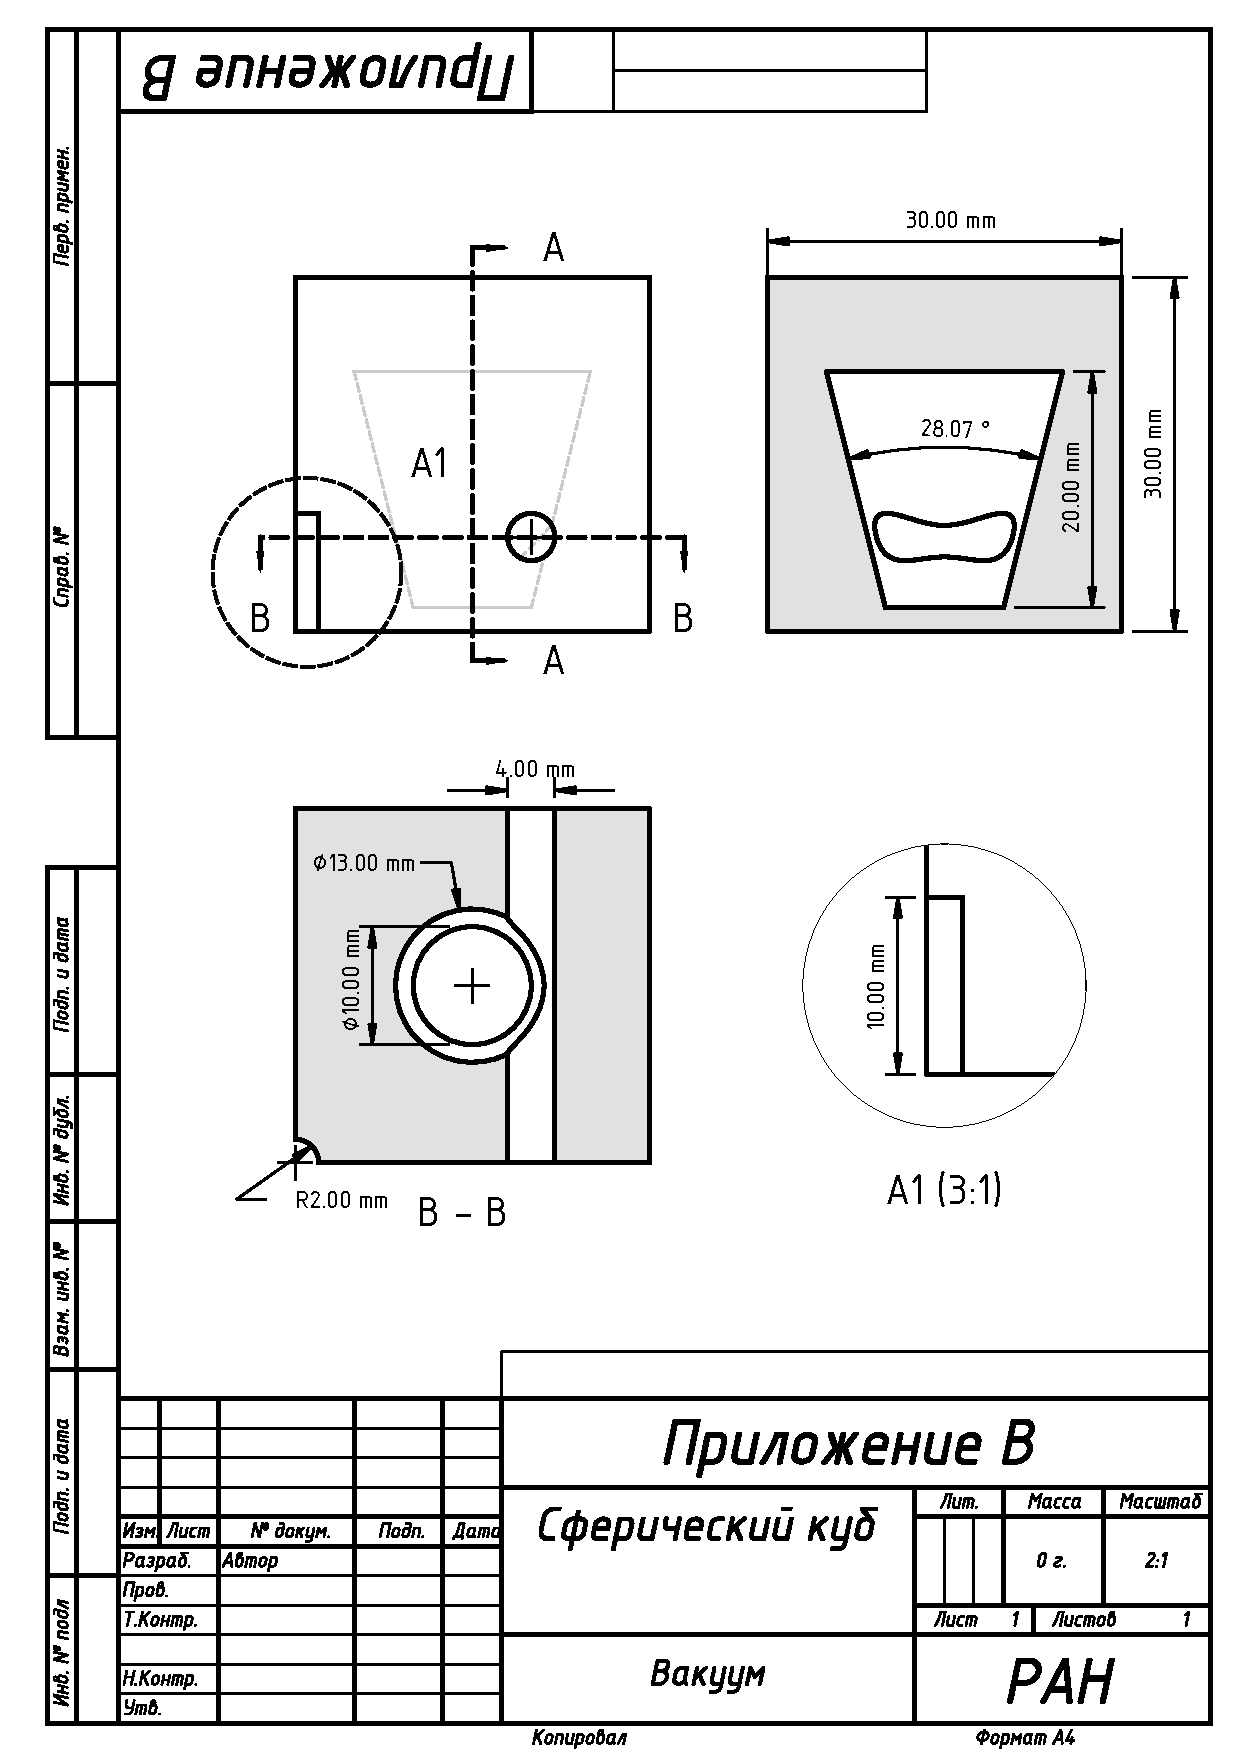
\includepdf[pages=-]{Dissertation/images/drawing.pdf}
        % Приложения

\end{document}
